\documentclass[oneside,fontsize=11pt,paper=a4]{scrartcl}
\usepackage[margin=1.5cm]{geometry}
\usepackage[utf8]{inputenc}
\usepackage[english]{babel}
\usepackage[autostyle]{csquotes}
\usepackage{url}
\usepackage{hyperref}
\usepackage{siunitx}
\usepackage{hyperref}
\usepackage{amsfonts}
\usepackage{amsmath}
\usepackage{amssymb}
\usepackage{multicol}
\usepackage{enumitem}
\usepackage{graphicx}
\usepackage{mathtools}
\usepackage{bm}
\usepackage{url}
\usepackage{xcolor}
\usepackage{soul}
\usepackage{tabularx}
\usepackage{makecell}
\usepackage{wrapfig}

\usepackage{stackengine}
\usepackage{scalerel}
\usepackage{xcolor,amssymb}


\geometry{footskip=1cm}

\urlstyle{same}
\setlength\parindent{0pt}
\setlist[description]{font=\normalfont\bfseries, style=unboxed}

% Kronecker Product
\newcommand{\A}[5]{\left#1\begin{array}{ccc}
{#2}_{11}\mathbf{B} & \cdots & {#2}_{1#4}\mathbf{B}\\
\vdots & \ddots & \vdots\\
{#2}_{#31}\mathbf{B} & \cdots & {#2}_{#3#4}\mathbf{B}
\end{array}\right#5}

\newcommand{\hlc}[2][yellow]{ {\sethlcolor{#1} \hl{#2}} }
\newcommand{\mathcolorbox}[2]{\colorbox{#1}{$\displaystyle #2$}}
\newcommand*{\Scale}[2][4]{\scalebox{#1}{$#2$}}%

\newcommand\norm[1]{\left\lVert#1\right\rVert}


\newcolumntype{Y}{>{\centering\arraybackslash}X}

\newenvironment{myfigure}
  {\par\medskip\noindent\minipage{\linewidth}}
  {\endminipage\par\medskip}

\title{Computer Vision 2 - Multiple View Geometry (IN2228)}
\author{Philipp Wulff \\ Technical University of Munich \\}
\date{Summer Semester 2023}

\begin{document}
\maketitle

\begin{abstract}
\noindent This summary covers the lecture ``Computer Vision 2 - Multiple View Geometry''  by Prof.\ Daniel Cremers and  Dr.\ Haoang Li. It builds on the summaries by Marcel Brucker and Franz Kaschner. 
\end{abstract}

% #############################
% ### LINEAR ALGEBRA ##########
% #############################


\begin{multicols}{2}[\section{Mathematical Background: Linear Algebra \& Calculus}]
\subsection{Set}
A Set $S$ of different elements e.g.\ the natural numbers $\mathbb{N} = \{1, 2, \dots\}$ or all real $n \times n$ matrices $\mathcal{M}(n)$.

\paragraph{Vector Space} A set $V$ is called a vector space over the field $\mathbb{R}$ if it is closed under
\begin{itemize}
    \setlength\itemsep{-0.2em}
    \item vector summation: $+: V \times V \rightarrow V$  and 
    \item scalar multiplication: $\cdot: \mathbb{R} \times V \rightarrow V$
\end{itemize}

\subsection{Transformations}
\begin{center}
    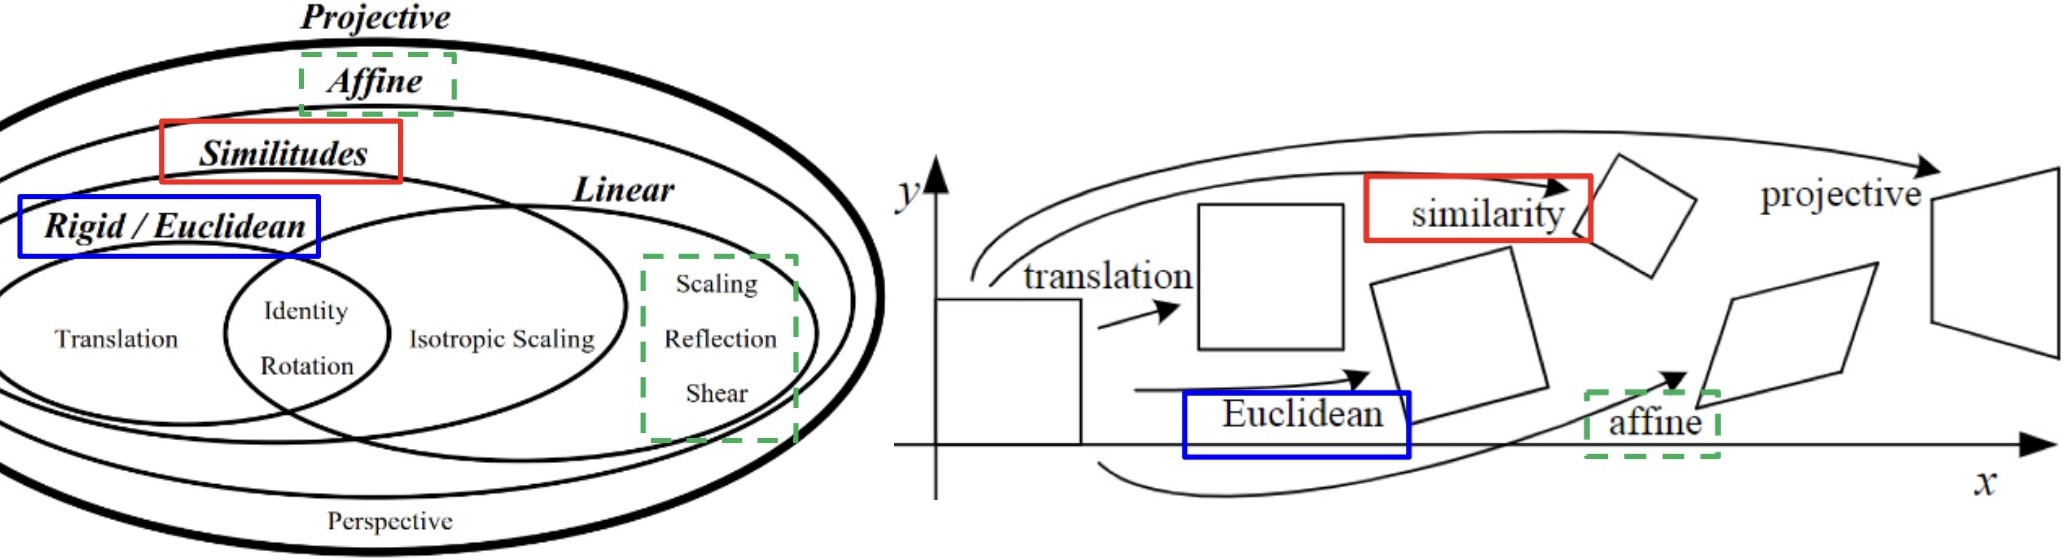
\includegraphics[width=\linewidth]{CV2-Latex-summary/Images/Transformations.jpg}
\end{center}
Linear: Origin remains unchanged.\\
Affine: Linear with/without Translation.

\paragraph{Linear Transformations} A linear transformation between two linear spaces is a map $L: V \rightarrow W$ with:
\begin{itemize}
    \setlength\itemsep{-0.2em}
    \item $L(x+y)=L(x)+L(y), \quad\forall x,y \in V$
    \item $L(\alpha x) = \alpha L(x), \quad\forall x \in V, \alpha \in \mathbb{R} $
\end{itemize}

\subsection{Linear Span and Linear Independence}
Given a set of vectors $S = \{v_1, \dots, v_k \} \subset V$, the linear span of $S$ is formed by all linear combinations:
\begin{equation*}
	\text{span}(S) = \left\{ v \in V \,\middle\vert\, v = \sum_{i=1}^k \alpha_i v_i \right\}
\end{equation*}
Linear independence holds if none of the vectors can be expressed as a linear combination of the remaining vectors. In $\mathbb{R}^3$, row reduce the matrix $S = \begin{psmallmatrix} \mathbf{v}^T_1\\ \mathbf{v}^T_2\\\mathbf{v}^T_3\end{psmallmatrix}$ using \textit{Gauss-Jordan elimination}.
If there is an all-zero row, the set is linearly dependent. Alternatively, \textbf{check if the determinant $\det(S) = 0$ is zero}. If so, $\mathbf{v}_1$, $\mathbf{v}_2$ and $\mathbf{v}_3$ are linearly independent. Linear dependence for a set of vectors holds if:
\begin{equation*}
	\sum_{i=1}^{n} \alpha_i \mathbf{v}_i = \mathbf{0} \quad \alpha_i \in \mathbb{R} \quad \text{(not all zero)}, \mathbf{v}_i \in \mathbb{R}^n
\end{equation*}

\subsection{Basis}
A set of vectors $B = {\mathbf{v}_1, \dots, \mathbf{v}_n}$ is called a basis of $V$ if it is \textbf{linearly independent and spans the vector space $V$}. A basis is a maximal set of linearly independent vectors. Properties for two bases ($B$ and $B'$) of a linear space $V$:
\begin{itemize}
	\item $B$ and $B'$ contain the same number of vectors, which is called the dimension of the space $V$.
	\item Any vector can be uniquely expressed as a linear combination of the basis vectors.
	\item All vectors can be expressed as linear combination of vectors of another basis.
\end{itemize}
The Gram–Schmidt process is a method for ortho-normalizing a set of vectors $\{\mathbf{v}_1, ..., \mathbf{v}_n\}$:
\begin{enumerate}
    \item Compute the orthogonal basis: 
        \begin{enumerate}
            \item First basis vector as $\mathbf{u}_1=\mathbf{v}_1$
            \item Then: $\mathbf{u}_k=\mathbf{v}_k-\sum^{k-1}_{j=1}\text{proj}_{\mathbf{u}_j}(\mathbf{v_k})$
            \item Stop for $k$ independent basis vectors.
        \end{enumerate}
    \item Normalize the orthogonal basis.
\end{enumerate}


%%% BEGIN MATRIX PROPERTIES %%%


\subsection{Matrix Properties}

\subsubsection{Determinant}

\begin{center}
    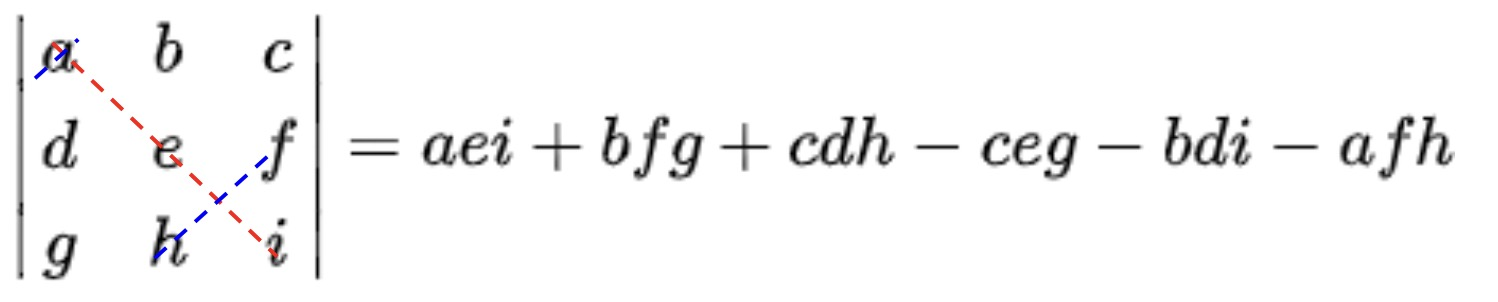
\includegraphics[width=0.8\linewidth]{CV2-Latex-summary/Images/Determinant.jpg}
\end{center}

\setlength{\columnsep}{0cm}
\begin{wrapfigure}{r}{0.4\linewidth}
    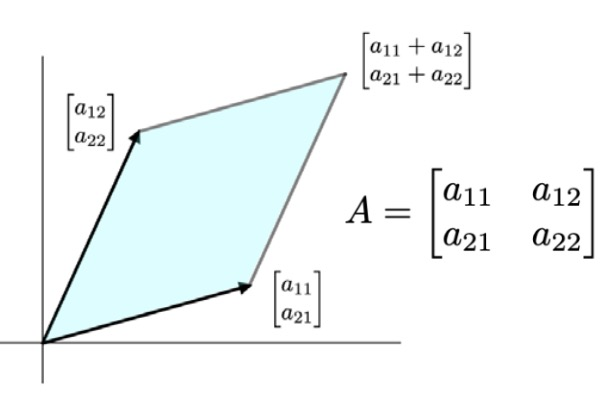
\includegraphics[width=\linewidth]{CV2-Latex-summary/Images/DeterminantParallelogram.jpg}
\end{wrapfigure}
Geometrically, $\vert\det\mathbf{A}\vert$:
is the \textbf{area of a parallelogram in 2D} and the \textbf{volume of a parallelepiped in 3D}. Properties:
\begin{itemize}
    \setlength\itemsep{-0.2em}
    \item $\det(c\mathbf{A})=c^n\det(\mathbf{A})$ 
    \item $\det{(\mathbf{A}^T)}=\det(\mathbf{A})$
    \item $\det{(\mathbf{AB})}=\det(\mathbf{A})\det(\mathbf{B})$
    \item $\det{(\mathbf{A}^{-1})}=\det(\mathbf{A})^{-1}$
\end{itemize}

\subsubsection{Range/Span}
A matrix's range is the span of its column vectors:
\begin{equation*}
\text{range}(\mathbf{A}) = \{ \mathbf{y} \in \mathbb{R}^m \ \vert \ \exists \mathbf{x} \in \mathbb{R}^n: \mathbf{A}\mathbf{x}=\mathbf{y} \}
\end{equation*}

\subsubsection{Rank}
The rank of a matrix is the dimension of its range: $\text{rank}(\mathbf{A}) = \text{dim}(\text{range}(\mathbf{A}))$. For $\mathbf{A} \in \mathbb{R}^{m \times n}$:
\begin{itemize}
    \setlength\itemsep{-0.1em}
    \item $\text{rank}(\mathbf{A}) = n - \text{dim}(\text{ker}(\mathbf{A}))$
    \item $0 \leq \text{rank}(\mathbf{A}) \leq \min\{m, n\}$
    \item $\text{rank}(\mathbf{A})$ is equal to the maximum number of linearly independent rows or columns of $\mathbf{A}$.
    \item Sylvester's inequality ($B \in \mathbb{R}^{n \times n}$): {\small$\text{rank}(A) + \text{rank}(\mathbf{B}) - n \leq \text{rank}(\mathbf{AB}) \leq \min\{\text{rank}(\mathbf{A}), \text{rank}(\mathbf{B})\}$}
    \item For any invertible matrices $\mathbf{C} \in \mathbb{R}^{m \times m}$ and $\mathbf{D} \in \mathbb{R}^{n \times n}$, we have: $\text{rank}(\mathbf{A}) = \text{rank}(\mathbf{CAD})$.
\end{itemize}

\subsubsection{Kernel/Null Space}
The null space or kernel of a matrix $\mathbf{A} \in \mathbb{R}^{n\times m}$ is  the subset of vectors $\textbf{x} \in \mathbb{R}^m$ which are mapped to zero:
\begin{equation*}
    \text{null}(\mathbf{A}) \equiv \text{ker}(\mathbf{A}) = \{\mathbf{x} \in \mathbb{R}^m \mid \mathbf{A}\mathbf{x} = \mathbf{0} \}
\end{equation*}

The LGS $\mathbf{A}\mathbf{x} = \mathbf{b}$ has a non-zero (non-trivial) solution iff $\mathbf{b} \in \text{range}(\mathbf{A})$. Properties:
\begin{itemize}
    \setlength\itemsep{-0.1em}
    \item $\det(\mathbf{A}) \neq 0 \Leftrightarrow \text{rank} (\mathbf{A}) = n \Leftrightarrow \text{ker}(\mathbf{A}) = \{0\}$
    \item $m = \text{rank}(\mathbf{A}) + k$, where k is the null space dimension and $m$ is the number of unknowns.
\end{itemize}

\subsubsection{Skew-symmetric Matrices}
A matrix $\mathbf{A} \in \mathbb{R}^{n \times n} $ is called skew-symmetric if $\mathbf{A}^T = -\mathbf{A}$ (meaning: $a_{ii} = 0$ and $a_{ij} = - a_{ji}$).
\begin{itemize}
    \setlength\itemsep{-0.1em}
    \item All eigenvalues are all zero or purely imaginary.
    \item There exist an orthogonal matrix $\mathbf{V}$ and block-diagonal matrix $\mathbf{\Lambda}$ such that $\mathbf{A} = \mathbf{V} \mathbf{\Lambda} \mathbf{V}^T$.
    \item The rank of any skew-sym.\ matrix is even. A $3\times3$ skew-symmetric matrix has rank $2$ or $0$.
\end{itemize}

\subsubsection{Eigenvalues and Eigenvectors}
Let $\mathbf{A} \in \mathbb{C}^{n \times n}$ be a complex matrix. A non-zero vector $\mathbf{v} \in \mathbb{C}^{n}$ is called a (right) eigenvector of $\mathbf{A}$ if:
\begin{equation*}
    \mathbf{A}\mathbf{v} = \lambda \mathbf{v} \ \text{with } \lambda \in \mathbb{C}, \mathbf{v} \neq 0.
\end{equation*}
\begin{itemize}
    \setlength\itemsep{-0.1em}
    \item The eigenvectors of a matrix $\mathbf{A}$ associated with different eigenvalues are linearly independent: $\lambda_a \neq \lambda_b \Rightarrow$ $\mathbf{v_a}$ and $\mathbf{v_b}$ are linearly independent
    \item All eigenvalues $\sigma (\mathbf{A})$ are the roots of the characteristic polynomial $\det(\mathbf{A}-\lambda \mathbf{I}) = \mathbf{0}$.
    \item If $\mathbf{A} = \mathbf{P}\mathbf{B}\mathbf{P}^{-1}$ for some non-singular matrix $\mathbf{P}$, then $\sigma (\mathbf{B}) = \sigma (\mathbf{A})$.
    \item $\sigma (\mathbf{A}) = \sigma (\mathbf{A}^T)$.
    \item $\mathbf{A}$ is symmetric and PD (or $\mathbf{U} = \mathbf{V}$) $\Rightarrow$ Eigendecomposition and SVD are equivalent.
    \item \textit{Geometrically},  eigenvectors are the vectors that are stretched, but not rotated by $\mathbf{A}$. E.g.\ for $\mathbf{A}\in\mathbb{R}^{2\times2}$, the eigenvectors are the two spatial directions in which every point slides in them.
\end{itemize}
Eigendecomposition ($\mathbf{A}, \mathbf{V}, \mathbf{\Lambda} \in \mathbb{R}^{n \times n}$):
\begin{equation*}
	\mathbf{A} = \mathbf{V} \Lambda \mathbf{V}^{-1}, \ \mathbf{\Lambda} = \text{diag}(\lambda_1, ..., \lambda_n),\
	\mathbf{V} =
	\begin{psmallmatrix}
		\vert &  & \vert \\
		\mathbf{v_1} & \cdots  & \mathbf{v_n} \\
		\vert &  & \vert \\
	\end{psmallmatrix}
\end{equation*}
$\mathbf{A}^{-1} = \mathbf{V} \Lambda^{-1} \mathbf{V}^{-1}$ if the eigen-decomposition exists and $\forall\lambda_i\neq0$.

\subsubsection{Orthogonality}

A matrix $\mathbf{A}$ is orthogonal iff its columns \textit{and} rows are orthogonal, i.e.\  $\mathbf{A}^T\mathbf{A}=\mathbf{A}\mathbf{A}^T=\mathbf{I}$. The determinant of an orthogonal matrix is $\pm 1$. It is column-orthogonal iff $\mathbf{A}^T\mathbf{A}=\mathbf{I}$. Property: $\mathbf{A}^T=\mathbf{A}^{-1}$.

\subsubsection{Singular Value Decomposition (SVD)}
Definitions differ in the shape of $\mathbf{\Sigma}$. Let $\mathbf{A} = \mathbf{U} \mathbf{\Sigma} \mathbf{V}^T \in \mathbb{R}^{m \times n}$ with $p = \text{rank}(\mathbf{A}) \leq \min(m,n)$. 
\begin{flalign*}
    \text{\textbf{Compact SVD:}}\quad
    \begin{aligned}
        &\mathbf{U} \in \mathbb{R}^{m \times p} \text{ (orthogonal columns)},\\
        &\mathbf{\Sigma}=\text{diag}(\sigma_1, ... , \sigma_p) \in \mathbb{R}^{p \times p}\text{ and}\\
        &V \in \mathbb{R}^{n \times p} \text{ (orthogonal)}\\   
    \end{aligned}
\end{flalign*}
where singular values are ordered: $\sigma_1 \geq ... \geq \sigma_n > 0$. SVD is a \textbf{generalization of eigenvalues and eigenvectors to non-square matrices}. The rank of $\mathbf{A}$ equals the number of non-zero singular values. Full SVD also contains the zero-singular-values:

\begin{flalign*}
    \text{\textbf{Full SVD:}}\quad
    \begin{aligned}
        &\mathbf{U} \in \mathbb{R}^{m \times m} \text{ (orthogonal),}\\
        &\mathbf{\Sigma}=\text{diag}(\sigma_1, ... , \sigma_p)=\begin{psmallmatrix} \mathbf{D}_{r\times r} & \mathbf{0}\\\mathbf{0}&\mathbf{0}\\\end{psmallmatrix} \in \mathbb{R}^{m \times n},\\
        &V \in \mathbb{R}^{n \times n} \text{ (orthogonal)}\\
    \end{aligned}
\end{flalign*}

\paragraph{Connection to the Eigendecomposition} 
\begin{flalign*}
    &\mathbf{A}^T \mathbf{A} = (\mathbf{V} \mathbf{\Sigma}^T \mathbf{U}^T) (\mathbf{U} \mathbf{\Sigma} \mathbf{V}^T) = \mathbf{V} \mathbf{\Sigma}^T \mathbf{\Sigma} \mathbf{V}^T
    \\
    &\mathbf{A} \mathbf{A}^T = (\mathbf{U} \mathbf{\Sigma} \mathbf{V}^T) (\mathbf{V} \mathbf{\Sigma}^T \mathbf{U}^T) = \mathbf{U} \mathbf{\Sigma} \mathbf{\Sigma}^T \mathbf{U}^T
\end{flalign*}
Thus, the columns of $\mathbf{V}$ and $\mathbf{U}$ are the Eigenvectors of $\mathbf{A}^T \mathbf{A}$ and $\mathbf{A} \mathbf{A}^T$ respectively. With  $\lambda_1\geq...\geq\lambda_r>0$ as the the non-zero Eigenvalues of $\mathbf{A} \mathbf{A}^T$ or $\mathbf{A}^T \mathbf{A}$, we conclude: $\mathbf{D}_{r\times r}=\begin{psmallmatrix} \sqrt{\lambda_1} & & \\  & \ddots & \\ & & \sqrt{\lambda_r} \end{psmallmatrix}$.

\paragraph{Applications} Given a matrix $\mathbf{A}$, SVD is useful for finding an orthogonal basis that stays orthogonal after transforming it with $\mathbf{A}$. It can also be used to map points on a circle onto points on a sphere.

\subsubsection{Pseudo Inverse (Generalized Inverse)}
Let $\mathbf{A} \in \mathbb{R}^{m \times n}$, $\mathbf{V} \in \mathbb{R}^{n \times n}$, $\mathbf{\Sigma} \in \mathbb{R}^{m \times n}$ and $\mathbf{U} \in \mathbb{R}^{m \times m}$.
$\mathbf{\Sigma}_1$ is the diagonal matrix of non-zero singular values. Then:
\begin{equation*}
    \mathbf{A}^+ = (\mathbf{A}^T \mathbf{A})^{-1} \mathbf{A}^T = \mathbf{V} \mathbf{\Sigma}^+ \mathbf{U}^T \text{ with } \mathbf{\Sigma}^+ = \begin{psmallmatrix} \mathbf{\Sigma}_1^{-1} & \mathbf{0}\\ \mathbf{0}&\mathbf{0}\\ \end{psmallmatrix}
\end{equation*}
$\mathbf{x} = \mathbf{A}^+ \mathbf{b}$ is the least squares solution of $\mathbf{A}\mathbf{x} = \mathbf{b}$.

\subsubsection{QR Decomposition}
$\mathbf{A}=\mathbf{Q}\mathbf{R}$, where $\mathbf{Q}$ is an orthogonal matrix and $\mathbf{R}$ is an upper triangular matrix. We find $\mathbf{Q}=[\mathbf{e}_1\dots\mathbf{e}_n]$ by applying the Gram-Schmidt process to $\mathbf{A}=[\mathbf{a}_1\dots\mathbf{a}_n]$. We obtain $\mathbf{R}$ by expressing the columns of $\mathbf{A}$ in the new basis and computing the ``similarity'' with the basis vectors:
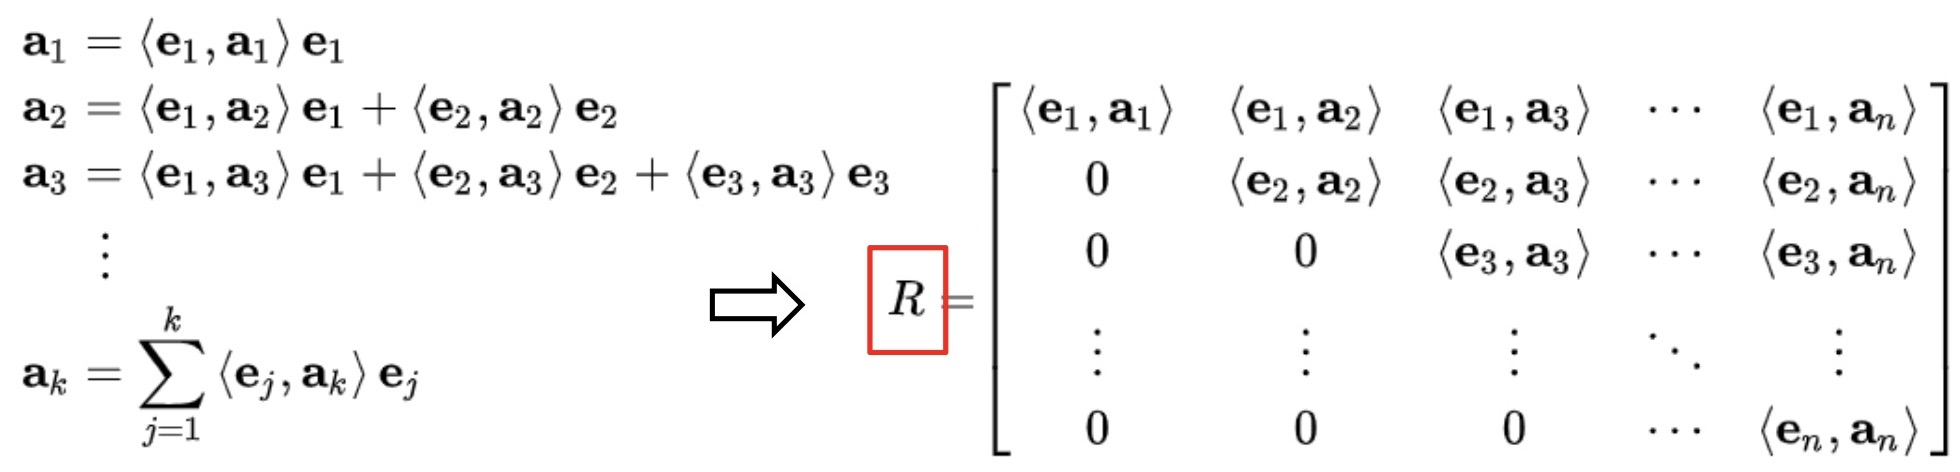
\includegraphics[width=\linewidth]{CV2-Latex-summary/Images/QRDecomposition.jpg}

\subsubsection{Symmetric Matrices}
A matrix $\mathbf{S} \in \mathbb{R}^{n \times n}$ is called symmetric if $\mathbf{S}^T = \mathbf{S}$.
\begin{itemize}
    \setlength\itemsep{-0.1em}
    \item All eigenvalues of $\mathbf{S}$ are real, i.e. $\sigma(\mathbf{S}) \subset \mathbb{R}$.
    \item Eigenvectors of $\mathbf{S}$ corresponding to the same distinct eigenvalues are orthogonal.
    \item There exist $n$ orthonormal eigenvectors of $\mathbf{S}$ which form a basis of $\mathbb{R}^3$. $\mathbf{S} = \mathbf{V \Lambda V}^T$ with $\mathbf{V} = (v_1, ..., v_n) \in O(n)$ and $\mathbf{\Lambda} = \text{diag}(\lambda_1, ..., \lambda_n)$.
    \item $\mathbf{S}$ is PD (PSD), if all eigenvalues are positive (and non-zero).
    \item Let $\mathbf{S}$ be positive semi-definite and $\lambda_1, \lambda_n$ the largest and smallest eigenvalue. Then $\lambda_1 = \max_{|x|=1} \langle x, \mathbf{S}x \rangle$ and $\lambda_n = \min_{|x|=1} \langle x, \mathbf{S}x \rangle$.
\end{itemize}


%%% END MATRIX PROPERTIES %%%

\subsection{Matrix Operations}

\subsubsection{Dot Product}

The dot product (\textit{inner product}) $\langle \cdot, \cdot \rangle: V \times V \rightarrow \mathbb{R}$ measures how similar two normalized vectors are.
\begin{equation*}
    \langle \mathbf{a}, \mathbf{b} \rangle = \mathbf{a}^T \mathbf
{b} = \norm{\mathbf{a}}\norm{\mathbf{b}}\cos\theta
\end{equation*}
Two vectors are orthogonal iff $\langle \mathbf{a}, \mathbf{b} \rangle = 0$ and point in the same direction iff $\langle \mathbf{a}, \mathbf{b} \rangle = 1$. Properties:
\begin{itemize}
    \setlength\itemsep{-0.1em}
	\item linear: $\langle c, \alpha a + \beta b \rangle = \alpha \langle c,a \rangle + \beta \langle c,b \rangle$ 
	\item symmetric: $\langle a,b \rangle = \langle b,a \rangle$
	\item positive definite: $\langle a, a \rangle \geq 0 $ and $ \langle a,a \rangle = 0 \iff v = 0$ 
\end{itemize}
\begin{multicols}{2}
    \begin{center}
        Projection of $\mathbf{b}$ onto $\mathbf{a}$:
        $$\text{proj}_\mathbf{a}\mathbf{b}=\frac
        {\mathbf{a}\cdot\mathbf{b}}{\norm{\mathbf{a}}}\underbrace{\frac{\mathbf{a}}{\norm{\mathbf{a}}}}_{\substack{\text{Unit vector}\\\text{along }\mathbf{a}}}$$
    \end{center}
    \hfill
    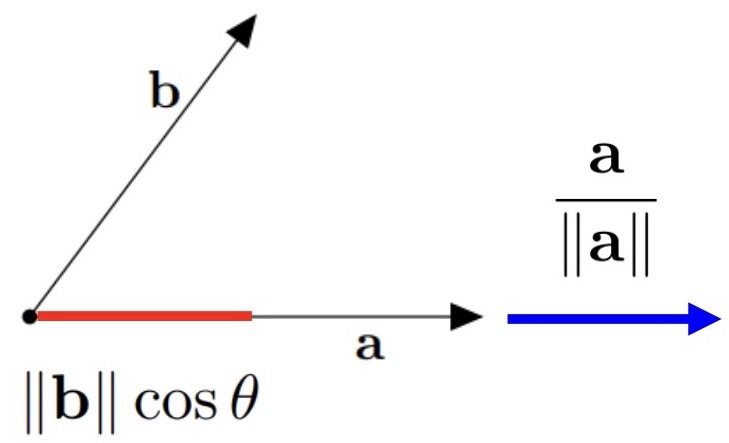
\includegraphics[width=4cm]{CV2-Latex-summary/Images/VecProjection.jpg}
\end{multicols}

\subsubsection{Cross product} \label{subsection:cross_product_skew}
On $\mathbb{R}^3$ we define the cross product as
\begin{equation*}
\begin{split}
    \times : \mathbb{R}^3 \times \, \mathbb{R}^3 \rightarrow \mathbb{R}^3: \underbrace{\mathbf{a} \times \mathbf{b}}_{= -\mathbf{b} \times \mathbf{a}} =  \begin{psmallmatrix} \mathbf{a}_2\mathbf{b}_3 - \mathbf{a}_3\mathbf{b}_2\\ \mathbf{a}_3\mathbf{b}_1 - \mathbf{a}_1\mathbf{b}_3\\
    \mathbf{a}_1\mathbf{b}_2 - \mathbf{a}_2\mathbf{b}_1 
    \end{psmallmatrix}
\end{split}
\end{equation*}
which is a vector orthogonal to $\mathbf{a}$ and $\mathbf{b}$. The right hand rule determines the direction.
\begin{wrapfigure}{r}{0.5\linewidth}
    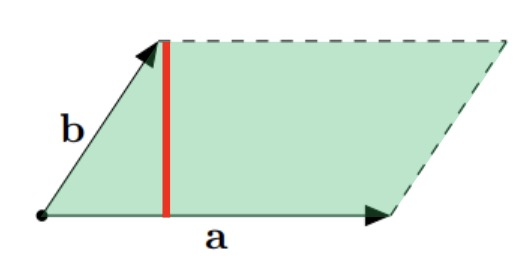
\includegraphics[width=\linewidth]{CV2-Latex-summary/Images/AreaParallelogram.jpg}
    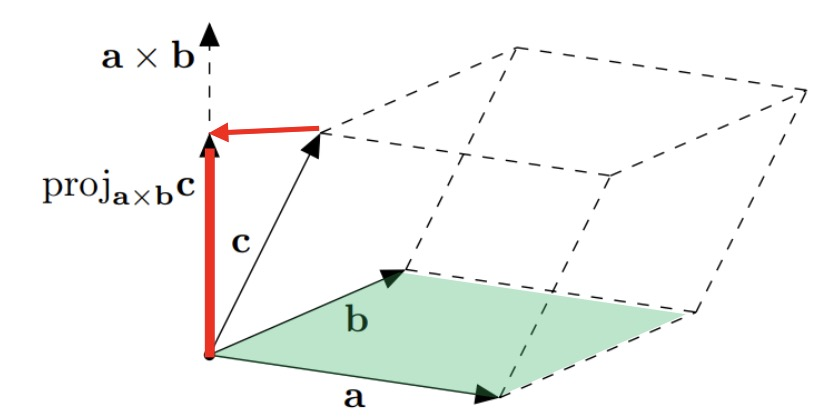
\includegraphics[width=\linewidth]{CV2-Latex-summary/Images/ParallelepipedVolume.jpg}
\end{wrapfigure}
We define the area of a parallelogram as
$\norm{\mathbf{a} \times \mathbf{b}}=\norm{\mathbf{a}}\norm{\mathbf{b}}\sin\theta$ and the volume of a parallelepiped as (Triple Product)

$$V=\norm{\mathbf{a} \times \mathbf{b}}\underbrace{\frac{(\mathbf{a} \times \mathbf{b})\cdot\mathbf{c}}{\norm{\mathbf{a} \times \mathbf{b}}}}_{\norm{\text{proj}_{\mathbf{a} \times \mathbf{b}}\mathbf{c}}}$$ 

The skew-symmetric matrix $\mathbf{[a]_\times} \in \mathbb{R}^{3 \times 3}$ replaces the cross product with matrix multiplication:
\begin{equation*}
     \mathbf{a} \times \mathbf{b} = \underbrace{\mathbf{[a]_\times}}_{\substack{\text{or }\mathbf{a}^\wedge\\\text{or }\mathbf{\hat{a}}}}\mathbf{b} = \begin{psmallmatrix} 0 & -a_3 & a_2\\ a_3 & 0 & -a_1\\ -a_2 & a_1 & 0 \end{psmallmatrix} \cdot \mathbf{b}.
\end{equation*}
The cross product of a vector with itself equals zero ($\mathbf{a} \times \mathbf{a} = 0$). Notation: $\mathbf{a}^\wedge=\mathbf{A}$ and $\mathbf{A}^{\vee}=\mathbf{a}$.

\subsubsection{Kronecker Product and Stack}
Given two matrices $\mathbf{A} \in \mathbb{R}^{m \times n}$, $\mathbf{B} \in \mathbb{R}^{k \times l}$, we define their Kronecker product:
\begin{flalign*}
	&\mathbf{A} \otimes \mathbf{B} \equiv {\footnotesize\A(amn) \in \mathbb{R}^{mk \times nl}} 
    \\
	&\text{with\quad}(\mathbf{A} \otimes \mathbf{B})^T = \mathbf{A}^T \otimes \mathbf{B}^T
\end{flalign*}

Given a matrix $\mathbf{A} \in \mathbb{R}^{m \times n}$, its stack $\mathbf{A}^S$ is obtained by stacking its $n$ column vectors $a_1, ..., a_n \in \mathbb{R}^{m}$:
\begin{equation*}
	\mathbf{A}^S \equiv 
	\begin{psmallmatrix}
		a_1 \\
		\vdots \\
		a_n \\
	\end{psmallmatrix}	
	\in \mathbb{R}^{mn}
    \quad\text{and}\quad
    u^T \mathbf{A} v = (v \otimes u)^T \mathbf{A}^S
\end{equation*}

\subsection{Group}
A group is an algebraic structure that combines a set $A$ and an operator $\circ$, e.g. $(\mathbb{N},\cdot)$, with the properties:
\begin{enumerate}
    \setlength\itemsep{-0.1em}
	\item $a \circ b \in S$ (Closure)
	\item $(a \circ b) \circ c = a \circ (b \circ c)$ (Associative law)
	\item $a \circ n = a$ ($n$ is an identity element in S)
	\item $a \circ a^{-1} = n$ (every element has an inverse element)
\end{enumerate}

Commutative addition of Abelian groups: $a \circ b = b \circ a$.

\paragraph{Ring} A set $S$ combined with two defined operations and properties from above, e.g. ($\mathbb{N}$, $+$, $\cdot$).

\paragraph{Field} A ring which is distributive in addition: $a \cdot (b + c) = a \cdot b + a \cdot c$, e.g. ($\mathbb{R}$, $+$, $\cdot$).

\paragraph{Popular Groups}
\begin{itemize}
    \setlength\itemsep{-0.1em}
    \item General linear group (matrix multiplication):\\
    $GL(n) = (\{\mathbf{A} \in \mathbb{R}^{n \times n} \; \vert \; \det(\mathbf{A}) \neq 0\}, \; \cdot \;)$
    \item Special linear group:\\
    $SL(n) = \{\mathbf{A} \in GL(n) \; \vert \; \det(\mathbf{A}) = +1\}$
    \item Orthogonal group (orth.\ matr.: $\det R = \pm1$):\\
    $O(n) = \left\{ \mathbf{R} \in GL(n) \; \vert \; \mathbf{R}^T\mathbf{R} = \mathbf{RR}^T = \mathbf{I} \right\}$
    \item Special orthogonal group (rot.\ matr.):\\
    $SO(n) = \{\mathbf{A} \in O(n) \; \vert \; \det(\mathbf{A}) = +1\}$
    \item Affine group (all affine transf.\ $L(\mathbf{x}) = \mathbf{Ax} + \mathbf{b}$):\\
    $A(n) = \{\begin{psmallmatrix} \mathbf{A} & \mathbf{b}\\ \mathbf{0}^T & 1\\ \end{psmallmatrix} \; \vert \; A \in GL(n), b \in \mathbb{R}^n\}$
    \item Euclidean group (subgroup of $A(n)$):\\
    $E(n) = \{\begin{psmallmatrix} \mathbf{R} & \mathbf{T}\\ \mathbf{0}^T & 1\\ \end{psmallmatrix} \; \vert \; \mathbf{R} \in O(n), \mathbf{T} \in \mathbb{R}^n\}$
    \item Special Euclidean group (Subgroup of $E(n)$):\\
    $SE(n) = \{\begin{psmallmatrix} \mathbf{R} & \mathbf{T}\\ \mathbf{0}^T & 1\\ \end{psmallmatrix} \; \vert \; \mathbf{R} \in SO(n), \mathbf{T} \in \mathbb{R}^n\}$\\
    Does rigid-body motions: $L(\mathbf{x}) = \mathbf{R}\mathbf{x} + \mathbf{T}$.
\end{itemize}
These groups are included in the following way:
\begin{flalign*}
    &SO(n) \subset O(n) \subset GL(n)
    \\
    &SE(n) \subset E(n) \subset A(n) \subset GL(n+1)
\end{flalign*}

\subsubsection{Subgroup test}
If $G$ is a group, and $H$ is a subset of $G$, then $H$ is a subgroup of $G$ iff $H$ is nonempty and closed under $\circ$ and inverses. Combination of these two conditions: For every $a$ and $b$ in $H$, the element $a \circ b^{-1}$ is in $H$.


\subsection{Norms for $A \in \mathbb{R}^{m \times n}$}
{\footnotesize\begin{flalign*}
    &\text{Induced 2-norm:}\;
	\norm{A}_2 = \max_{|x|_2 = 1} \sqrt{\langle x, A^T A x \rangle} = \sigma_1
    \\
	&\text{Frobenius norm:}\;
    \norm{A}_F = \sqrt{\sum_{i,j} a_{ij}^2} = \sqrt{\text{Tr}(A^T A)} = \sqrt{\sigma_1^2 + ... + \sigma_n ^2}
\end{flalign*}}
{\small
With $A^T A = V \cdot \text{diag}(\sigma_1^2, ..., \sigma_n^2) \cdot V^T$ and $\sigma_1^2 \geq \sigma_i^2 \geq 0$.
}
\subsection{Derivative, Gradient and Jacobian}

The \textbf{derivative} of a \textit{single univariate} function is:
\begin{flalign*}
    f'(x)=\frac{df}{dx}, \text{ where }x\in\mathbb{R}
    \quad\quad\text{with }f(x)\in\mathbb{R}.
\end{flalign*}
The \textbf{gradient} of a \textit{single multivariate} function is:
\begin{flalign*}
    \nabla f(x_1,x_2,...,x_n)=\begin{psmallmatrix}
        \frac{\partial f}{\partial x_1}\\
        \frac{\partial f}{\partial x_2}\\
        ...\\
        \frac{\partial f}{\partial x_n}
    \end{psmallmatrix}
    \quad\text{with }f(x_1,x_2,...,x_n)\in\mathbb{R}.
\end{flalign*}
The derivative of a \textit{multiple multivariate function} (vector-valued) is the \textbf{Jacobian}:

\begin{flalign*}
    \frac{\partial F}{\partial \mathbf{x}}=\begin{psmallmatrix}
        \frac{\partial F_1}{\partial \mathbf{x}_1} & ... & \frac{\partial F_1}{\partial \mathbf{x}_n} \\
        & \vdots &  \\
        \frac{\partial F_m}{\partial \mathbf{x}_1} & ... & \frac{\partial F_m}{\partial \mathbf{x}_n}
    \end{psmallmatrix}
    \quad\text{with }F(x_1,x_2,...,x_n)\in\mathbb{R}^m.
\end{flalign*}

\subsection{Taylor Approximation}

First-order Taylor polynomial around some value $a$:

\begin{flalign*}
    f(x)\vert_a\approx f(a)+\frac{f'(a)}{1!}(x-a)
\end{flalign*}

\subsection{Laplace Operator}

Mathematically, it is defined as:

\begin{flalign*}
    \nabla^2 f&=\frac{\partial^2 f}{\partial x^2} + \frac{\partial^2 f}{\partial y^2}
    \\
    &=[f(x+1,y)+f(x-1,y)+f(x,y+1)
    \\&\quad\quad+f(x,y-1)]-4f(x,y)
\end{flalign*}
where $\nabla^2$ is the Laplacian operator. The Laplace operator is used like a convolution kernel and highlights the pixels with sharp intensity discontinuity (e.g.\ edge or corner pixels). 

\begin{center}
    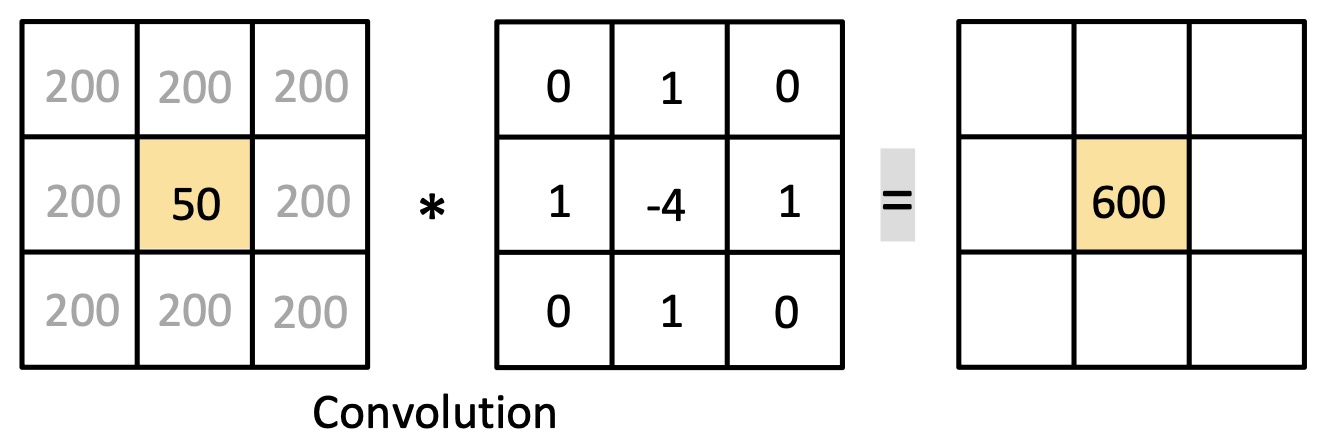
\includegraphics[width=0.55\linewidth]{CV2-Latex-summary/Images/LaplaceOperator.jpg}
    \hfill
    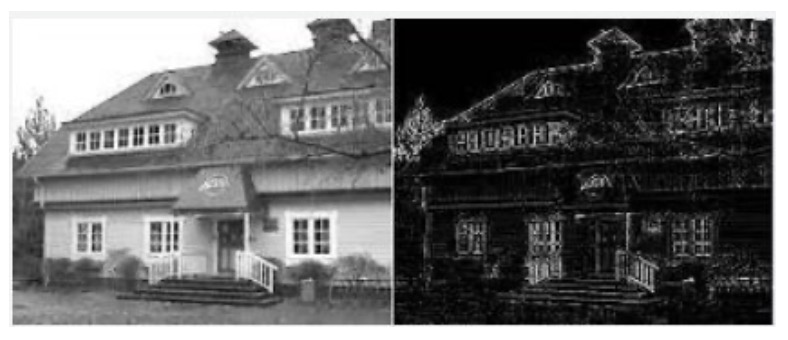
\includegraphics[width=0.4\linewidth]{CV2-Latex-summary/Images/LaplaceOperatorResult.jpg}
\end{center}

\end{multicols}

\newpage

% #######################################
% ### MOTION AND SCENE REPRESENTATION ###
% #######################################


\begin{multicols}{2}[\section{Motion and Scene Representation}]
\subsection{3D Space} \label{subsection:3d_space}
The three-dimensional Euclidean space $\mathbb{E}^3$ consists of all points $\mathbf{p} \in \mathbb{E}^3$ characterized by coordinates
\begin{equation*}
    \mathbf{X} \equiv (X_1, X_2, X_3)^T \in \mathbb{R}^3.
\end{equation*}
Given two points $\mathbf{X}$ and $\mathbf{Y}$, one can define a bound vector $\mathbf{v}$ as
\begin{equation*}
    \mathbf{v} = \mathbf{X} - \mathbf{Y} \in \mathbb{R}^3.
\end{equation*}

\subsection{Rigid Body Motion}
A rigid body motion is a map
\begin{equation*}
	g_t: \mathbb{R}^3 \rightarrow \mathbb{R}^3; \ \mathbf{X} \mapsto g_t(\mathbf{X}), \ t \in [0,T]
\end{equation*}
which preserves the norm and inner product (length), the cross product (orientation) and the triple product (volume) of any two vectors.
The rigid body motion can be written as $g_t(\mathbf{x}) = \mathbf{R}\mathbf{x} + \mathbf{T}$, where $\mathbf{R} \in SO(3)$ is a rotation matrix from the special orthogonal group and $\mathbf{T} \in \mathbb{R}^3$ is a translation vector.

\subsection{The Special Orthogonal Group: SO(3)}
The effect of any infinitesimal rotation $\mathbf{R} \in SO(3)$ can be approximated by an element from the space of skew-symmetric matrices $\mathfrak{so}(3) = \{\hat{w} \, \vert \, w \in \mathbb{R}^3\}$. The rotation group $SO(3)$ is called a Lie group and the linear space $\mathfrak{so}(3)$ is called its Lie algebra.

\paragraph{Definition ``Lie group'':} Smooth manifold that is also a group, s.t. the group operations multiplication and inversions are continuous (smooth) maps. The SO(n) and SE(n) groups are continuous in real space and are therefore Lie Groups.

\begin{flalign*}
    \text{SO}(n)=\{\mathbf{R}\in\mathbb{R}^{n\times n}\,\vert\,\mathbf{R}\mathbf{R}^T=\mathbf{I}, \det{(\mathbf{R})}=1\}
\end{flalign*}

\paragraph{Definition ``Lie algebra'':} The tangent space of a Lie group at the identity element is called the associated Lie algebra. While the multiplication operator is well-defined on the SO(3) group, the addition operator is not, which affects the derivative computation. We use the Lie algebra to obtain an expression for the derivative of rotation matrices from the SO(3) group.

\begin{flalign*}
    \mathfrak{so}(3)={\left\{w\in\mathbb{R}^{3}\;{\mathrm{or}}\;\hat{w}=\begin{psmallmatrix}{{0}}&{{-w_{3}}}&{{w_{2}}}\\ {{w_{3}}}&{{0}}&{{-w_{1}}}\\ {{-w_{2}}}&{{w_{1}}}&{{0}}\end{psmallmatrix}\in\mathbb{R}^{3\times3}\right\}}
\end{flalign*}

\begin{myfigure}
	\centering
	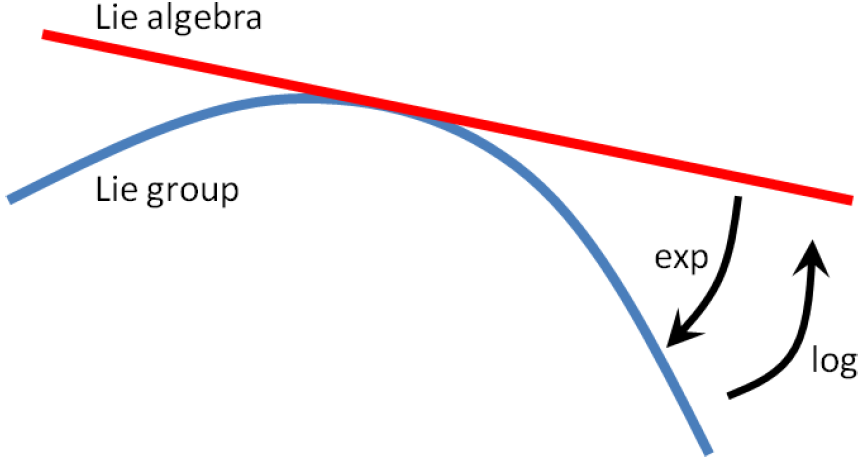
\includegraphics[width=0.6\linewidth]{Images/lie_group_algebra.PNG}
\end{myfigure}

The matrix exponential defines a map from the Lie algebra to the Lie group and, conversely, the logarithm maps elements in SO(3) to $\mathfrak{so}(3)$:
\begin{flalign*}
    &\exp: \mathfrak{so}(3) \rightarrow SO(3);\quad \hat{w} \mapsto \exp(\hat{w}) \; (= \mathbf{R})
    \\
    &\log: SO(3) \rightarrow \mathfrak{so}(3);\quad \mathbf{R} \mapsto \log(\mathbf{R}) \; (= \hat{w}).
\end{flalign*}
Where Rodrigues' formula gives the matrix exponential: 
\begin{equation*}
    \exp(\hat{w}) = \mathbf{I} + \frac{\hat{w}}{\theta} \sin(\theta) + \frac{\hat{w}^2}{\theta^2} \left(1-\cos\left(\theta\right)\right) = \mathbf{R}
\end{equation*}
and the inverse logarithmic mapping is given by:
\begin{equation*}
\begin{split}
   \theta = \norm{w} = \cos^{-1} \left(\frac{\text{tr}(\mathbf{R})-1}{2} \right) \quad\text{(angle)}\\ \frac{w}{\norm{w}} = \frac{1}{2\sin\left(\norm{w}\right)} \begin{pmatrix}r_{32} - r_{23}\\ r_{13} - r_{31}\\ r_{21} - r_{12} \end{pmatrix} \quad\text{(axis)}
\end{split}
\end{equation*}
for all $\mathbf{R} \neq \mathbf{I}$. If $w = 0$, we have $\exp(\hat{w}) = \mathbf{I}$. Any orthogonal transformation $\mathbf{R} \in SO(3)$ can be achieved by rotating about the angle $|w|$ around
an axis $\frac{w}{|w|}$.

\subsection{The Special Euclidean Group: SE(3)}
The space of rigid body motions given by the group of special euclidean transformations
\begin{equation*}
    SE(3) \equiv \left\{g = (\mathbf{R}, \mathbf{T}) \,\middle\vert\, \mathbf{R} \in SO(3), \mathbf{T} \in \mathbb{R}^3 \right\}.
\end{equation*}
In homogeneous coordinates, we have:
\begin{equation*}
    SE(3) \equiv \left\{g = \begin{pmatrix} \mathbf{R} & \mathbf{T}\\ \mathbf{0}^T & 1 \end{pmatrix} \,\middle\vert\, \mathbf{R} \in SO(3), \mathbf{T} \in \mathbb{R}^3 \right\} \subset \mathbb{R}^{4 \times 4}
\end{equation*}
And the set of all twists forms its Lie algebra $\mathfrak{se}(3)$:
\begin{equation*}
\begin{split}
    \mathfrak{se}(3) \equiv \left\{\mathbf{\hat{\xi}} = \begin{pmatrix} \mathbf{\hat{w}} & \mathbf{v}\\ \mathbf{0}^T & 0 \end{pmatrix} \,\middle\vert\, \mathbf{\hat{w}} \in \mathfrak{so}(3), \mathbf{v} \in \mathbb{R}^3 \right\} \subset \mathbb{R}^{4 \times 4}\\
    \text{with} \quad \mathbf{v}(t) = \mathbf{\dot{T}}(t) - \mathbf{\hat{w}}(t)\mathbf{T}(t)
\end{split}
\end{equation*}
where $v$ is the linear velocity and $w$ is the angular velocity. Operators $\wedge$ and $\vee$ convert between a twist $\hat{\xi} \in \mathfrak{se}(3)$ and its twist coordinates $\xi \in \mathbb{R}^6$:
\begin{flalign*}
    \hat{\xi} \equiv \begin{pmatrix} v\\w \end{pmatrix}^{\wedge} &\equiv \begin{pmatrix} \hat{w} & v\\0 & 0 \end{pmatrix} \in \mathbb{R}^{4 \times 4}\\
    \begin{pmatrix} \hat{w} & v\\0 & 0 \end{pmatrix}^{\vee} &= \begin{pmatrix} v\\ w \end{pmatrix} \in \mathbb{R}^6
\end{flalign*}
We define an exponential map from the Lie Algebra to the Lie Group $\exp: \mathfrak{se}(3) \rightarrow SE(3); \ \hat{\xi} \mapsto \exp(\hat{\xi})$:
\begin{flalign*}
    &\text{For $w = 0$:}\quad \exp(\hat{\xi}) = \begin{pmatrix}\mathbf{I} & \mathbf{v}\\ \mathbf{0}^T & 1 \end{pmatrix}
    \\
    &\begin{aligned}
        \text{For $w \neq 0$:}\quad \exp(\hat{\xi}) &= \begin{pmatrix}\exp(\hat{w}) & \mathbf{Vv}\\ \mathbf{0}^T & 1 \end{pmatrix} 
        = \begin{pmatrix}\mathbf{R} & \mathbf{T}\\\mathbf{0}^T & 1 \end{pmatrix} = g
    \end{aligned}
    \\
    &\text{with }\mathbf{V}=\mathbf{I}_3+\frac{1-\cos\theta}{\theta^2}\mathbf{\hat{w}}+\frac{\theta-\sin\theta}{\theta^3}\mathbf{\hat{w}}^2 
    \text{ and }\theta=\norm{\mathbf{w}}_2
\end{flalign*}

{\footnotesize More info: \url{http://ethaneade.com/lie.pdf} and \href{https://ingmec.ual.es/~jlblanco/papers/jlblanco2010geometry3D_techrep.pdf}{this tutorial}.} 

In summary:
\begin{center}
    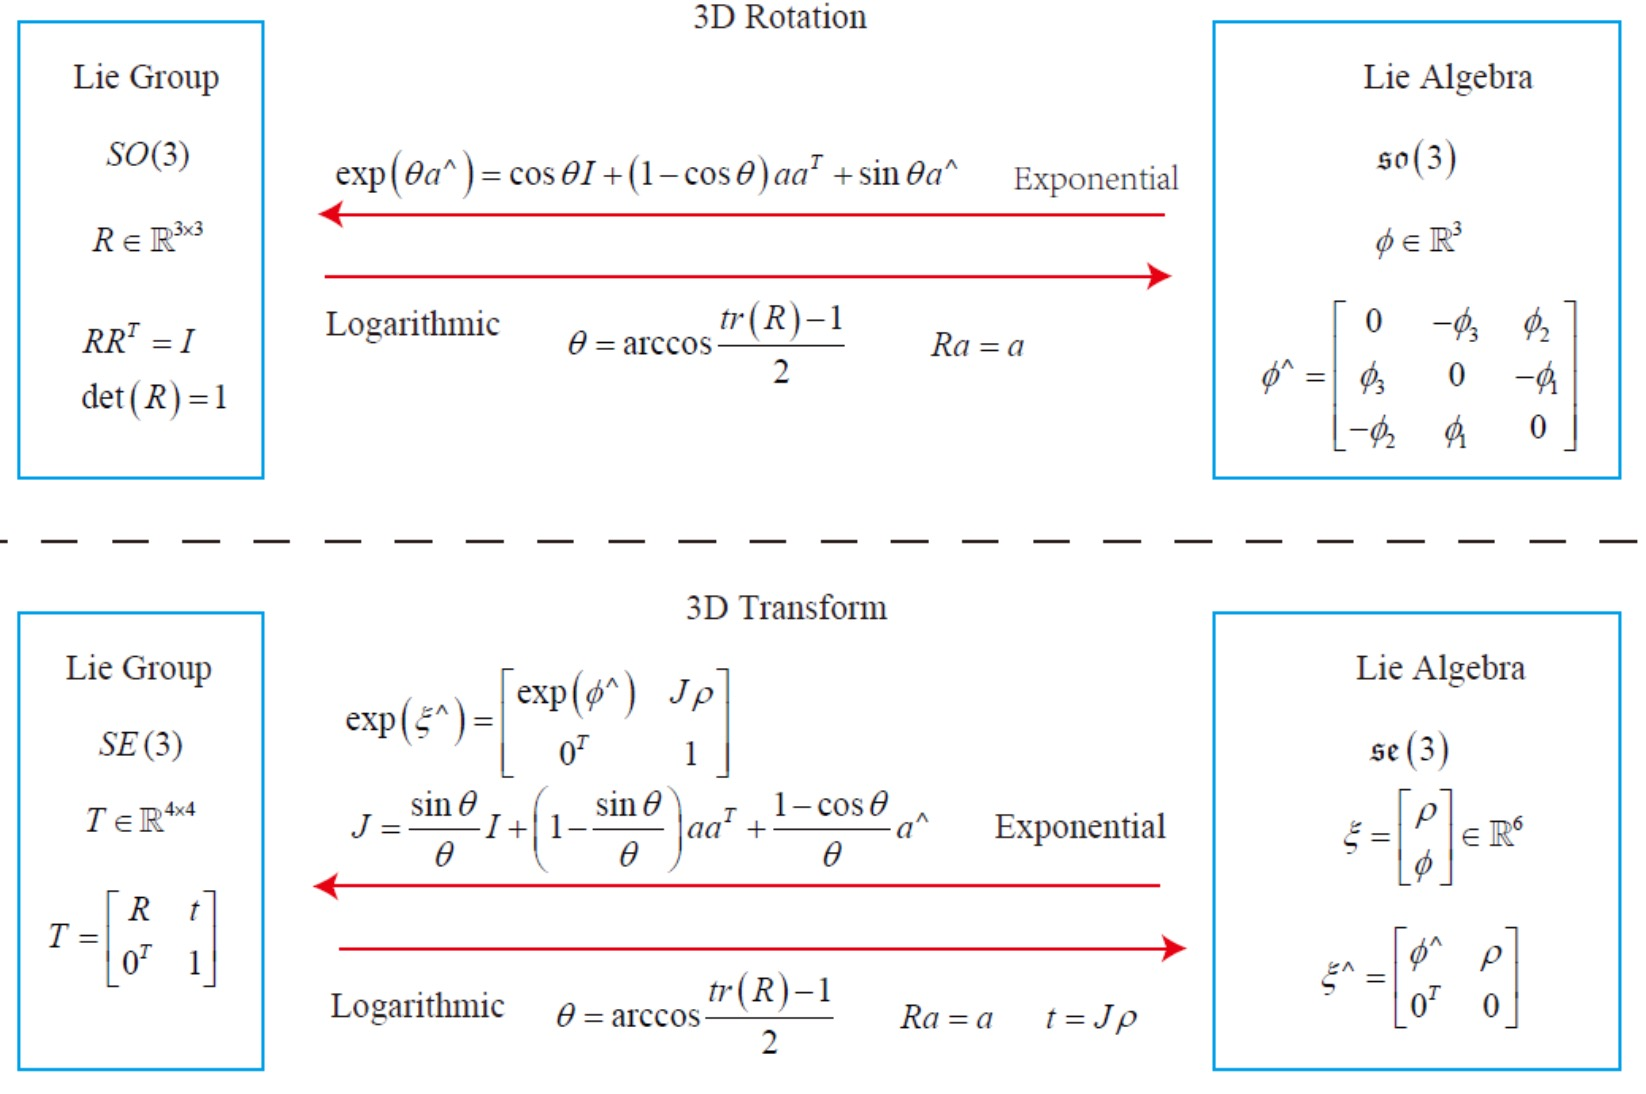
\includegraphics[width=\linewidth]{CV2-Latex-summary/Images/LieAlgebraScreenshot.jpg}
\end{center}

\subsection{BCH Formula}

We compute derivatives on $\mathfrak{so}(3)$ using the BCH formula. The problem is that the sum $\mathbf{R}_1+\mathbf{R}_2$ is not defined on SO(3) and it also does not directly correspond to the product of two vectors on $\mathfrak{so}(3)$.

\subsection{Representing the Camera Motion}
The rigid-body transformation
\begin{equation*}
    g(t) = \begin{pmatrix} \mathbf{R}(t) & \mathbf{T}(t)\\\mathbf{0}^T & 1 \end{pmatrix} \in SE(3)
\end{equation*}
represents the motion from a fixed world frame to the camera frame at time $t$.
In particular we assume that at time $t = 0$ the camera frame coincides with the world frame, i.e. $g(0) = \mathbf{I}$.
For any point $\mathbf{X}_0$ in world coordinates, its coordinates in the camera frame at time $t$ are:
\begin{equation*}
    \mathbf{X}(t) = \mathbf{R}(t)\mathbf{X}_0 + \mathbf{T}(t)
\end{equation*}
or in homogeneous representation
\begin{equation*}
    \mathbf{X}(t) = g(t)\mathbf{X}_0.
\end{equation*}
We denote the transformation from the points in frame $t_1$ to the points in frame $t_2$ by $g(t_2,t_1)$:
\begin{equation*}
    \mathbf{X}(t_2) = g(t_2, t_1)\mathbf{X}(t_1).
\end{equation*}
\begin{equation*}
    g(t_1, t_2)g(t_2, t_1) = I \Leftrightarrow g^{-1}(t_2, t_1) = g(t_1, t_2)
\end{equation*}
For velocity transformation it applies
\begin{equation*}
    \begin{split}
        \mathbf{\dot{X}}(t) = \hat{w}(t)\mathbf{X}(t) + v(t) \quad \text{or} \\ \mathbf{\dot{X}}(t) = \mathbf{\hat{V}}(t)\mathbf{X}(t) \quad \text{with} \\ \mathbf{\hat{V}}(t) = \begin{pmatrix}\hat{w}(t) & v(t)\\0 & 0 \end{pmatrix} \in se(3)
    \end{split}
\end{equation*}

\begin{center}
    We calculate \textbf{relative poses} from absolute poses:
    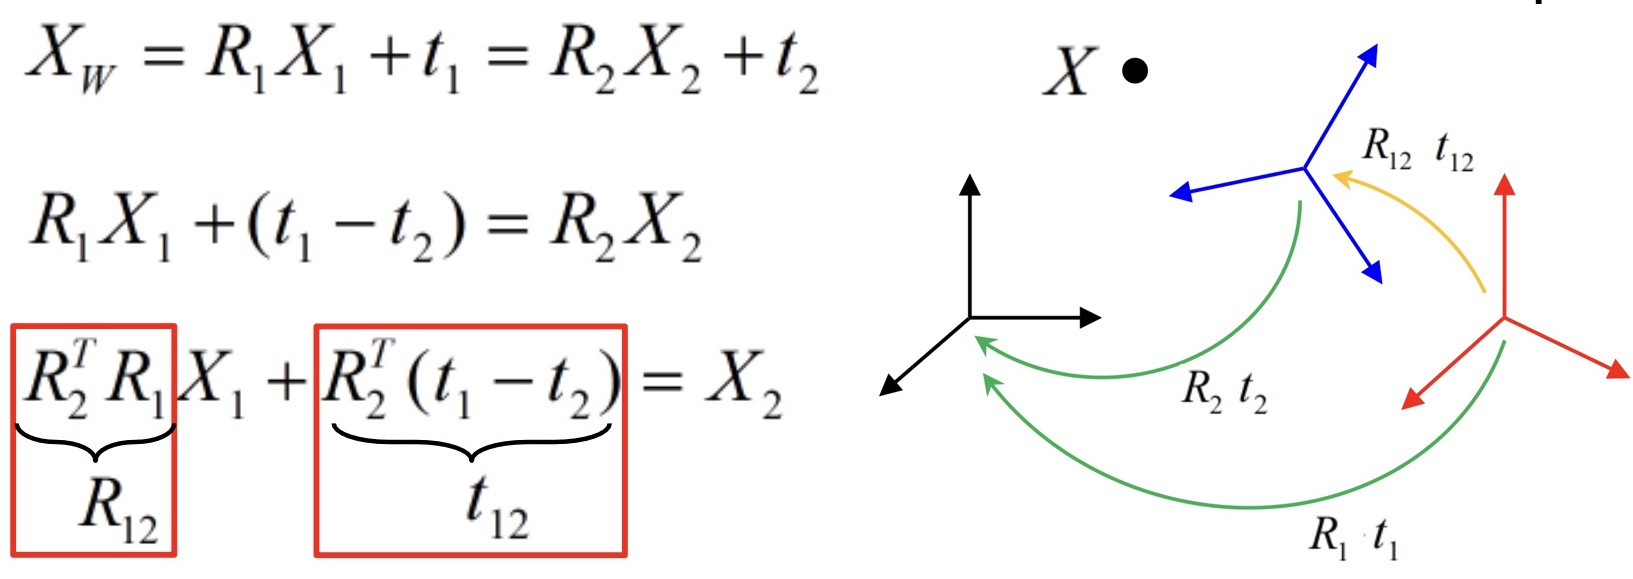
\includegraphics[width=\linewidth]{CV2-Latex-summary/Images/RelativePose.jpg}
\end{center}

We invert a tranformation via:
\begin{flalign*}        
    \mathbf{Y}=\mathbf{R}\mathbf{X}+\mathbf{t}\quad\Rightarrow\quad\mathbf{X}=\mathbf{R}^T(\mathbf{Y}-\mathbf{t})\\
    \mathbf{T}=\begin{pmatrix}\mathbf{R}^T&-\mathbf{R}^T\mathbf{t}\\\mathbf{0}^T&1\end{pmatrix}
\end{flalign*}

\subsection{Motion of A 3D Line}

\begin{wrapfigure}{r}{0.4\linewidth}
    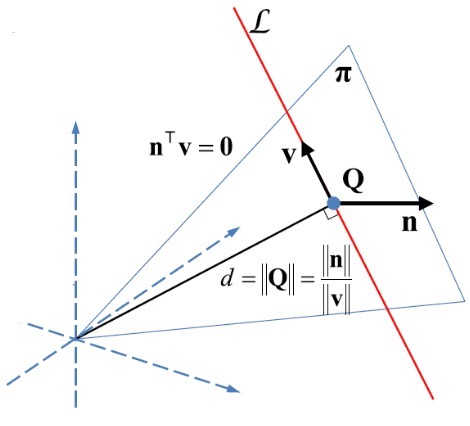
\includegraphics[width=\linewidth]{CV2-Latex-summary/Images/PluckerLine.jpg}
\end{wrapfigure}
We represent a 3D line using its \textit{Plücker Coordinates} $(\mathbf{v}, \mathbf{n})$, where $\mathbf{v}$ is the direction vector of the line and $\mathbf{n}=\mathbf{Q}\times\mathbf{v}$ is the normal of the projection plane that we calculate from the cross product with some point on the line $\mathbf{Q}$. Plücker coordinates have 4 DOF.

We transform a Plücker line from the ith to the jth coordinate frame via:
\begin{flalign*}
    \begin{pmatrix}\mathbf{n}_j\\\mathbf{v}_j\end{pmatrix}=
    \begin{pmatrix}\mathbf{R}_{ji}&[\mathbf{t}_{ji}]_\times\mathbf{R}_{ji}\\\mathbf{0}&\mathbf{R}_{ji}\end{pmatrix}
    \begin{pmatrix}\mathbf{n}_i\\\mathbf{v}_i\end{pmatrix}
\end{flalign*}
which changes the norm of $\mathbf{n}$ and not of $\mathbf{v}$.

\subsection{Similarity Transformation in 3D: Sim(3)}

We define 
\begin{flalign*}
    \mathbf{T}_S=\begin{pmatrix}s\mathbf{R}&\mathbf{t}\\\mathbf{0}^T&1\end{pmatrix}
\end{flalign*}
which is a 7 DOF transformation. The scale for the rotation enables matching of point clouds at different scales.


\subsection{Adjoint Map}
A viewer in frame $A$ is displaced relative to the current frame by a transformation $g_{xy}: Y = g_{xy} X(t)$.
The velocity in frame $A$ is then
\begin{equation*}
    \dot{Y}(t) = g_{xy} \dot{X}(t) = g_{xy} \hat{V}(t) X(t) = g_{xy} \hat{V} g_{xy}^{-1} Y(t).
\end{equation*}
This shows that the relative velocity of points observed from camera frame $A$ is represented by the twist
\begin{equation*}
    \hat{V}_y = g_{xy} \hat{V} g_{xy}^{-1} \equiv ad_{g_{xy}}(\hat{V})
\end{equation*}
with the adjoint map
\begin{equation*}
	ad_g: se(3) \rightarrow se(3); \ \hat{\xi} \mapsto g \hat{\xi} g^{-1}.
\end{equation*}

\subsection{More Ways of Expressing Rotation}

We differentiate extrinsic rotations about axes of the fixed, global coordinate system from intrinsic rotations about the dynamic coordinate system attached to a moving body. 

\subsubsection{Axis-Angle Representation}
\setlength{\columnsep}{0cm}
Rotation about $\theta$ around a unit vector $\mathbf{e}$, represented by the rotation vector $\mathbf{\theta e}=(\mathbf{e}, \theta)$. We  convert an axis-angle representation into a rotation matrix using Rodrigues' formula:
\begin{flalign*}
    \mathbf{R}&(\mathbf{n}, \theta)=\cos \theta \mathbf{I}+(1-\cos \theta) \mathbf{n n}^T+\sin \theta \mathbf{n}^{\wedge}\\
    &=\begin{psmallmatrix}
    n_x^2(1-c \theta)+c \theta & n_x n_y(1-c \theta)+n_z s \theta & n_x n_z(1-c \theta)-n_y s \theta \\
    n_x n_y(1-c \theta)-n_z s \theta & n_y^2(1-c \theta)+c \theta & n_y n_z(1-c \theta)+n_x s \theta \\
    n_x n_z(1-c \theta)+n_y s \theta & n_y n_z(1-c \theta)-n_x s \theta & n_z^2(1-c \theta)+c \theta
    \end{psmallmatrix}
\end{flalign*}
And vice versa:
{\small
\begin{flalign*}
    &\mathbf{n}=\frac{1}{2 \sin \theta}\begin{pmatrix}R_{32}-R_{23} \\R_{13}-R_{31} \\R_{21}-R_{12}\end{pmatrix},\quad\theta=\arccos \left(\frac{\operatorname{tr}(\mathbf{R})-1}{2}\right)
    \\
    &\begin{aligned}
        \operatorname{tr}(\mathbf{R}) & =\cos \theta \operatorname{tr}(\mathbf{I})+(1-\cos \theta) \operatorname{tr}\left(\mathbf{n n}^T\right)+\sin \theta \operatorname{tr}\left(\mathbf{n}^{\wedge}\right) \\
        & =3 \cos \theta+(1-\cos \theta) \\
        & =1+2 \cos \theta
    \end{aligned}
\end{flalign*}
}
The axis-angle representation has 4 parameters with one DOF removed due to the unit vector constraint.

\subsubsection{Quaternion}
\begin{multicols}{2}
    We define a rotation using a set of four numbers $\mathbf{q}=(q_0, q_1, q_2, q_3)$ that parameterize a complex number with three imaginary axes: $\mathbf{q}=q_0+q_1 \mathbf{i}+q_2 \mathbf{j}+q_3 \mathbf{k}$
    \hfill
    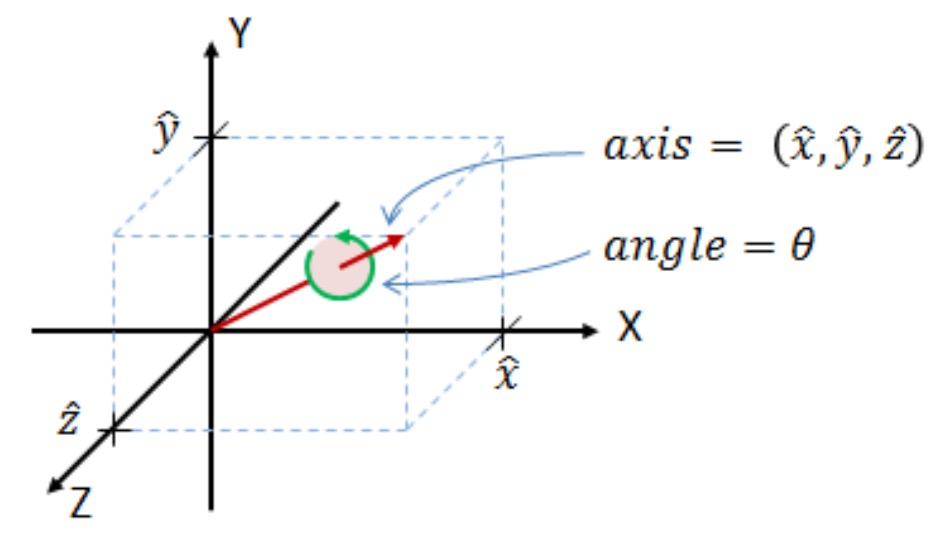
\includegraphics[width=4.5cm]{CV2-Latex-summary/Images/Quaternion.jpg}
\end{multicols}
\begin{flalign*}
    &q_0=\cos\left(\frac{\theta}{2}\right) \quad
    q_1=\hat{x}\sin\left(\frac{\theta}{2}\right) \quad
    q_2=\hat{y}\sin\left(\frac{\theta}{2}\right) 
    \\
    &q_3=\hat{z}\sin\left(\frac{\theta}{2}\right) \quad
    \mathbf{q}=[\underbrace{\cos\frac{\theta}{2}}_{\text{real}}, \underbrace{\mathbf{n}\sin\frac{\theta}{2}}_{\text{imaginary}}]
\end{flalign*}
3D points can be represented as quaternions with a zero-real-coordinate, $\mathbf{p}=(0,x,y,z)$. We convert quaternions to a rotation matrix using the \textit{Hamilton product} (derivation skipped):
\begin{flalign*}
    R=\begin{pmatrix}1-2\left(q_y^2+q_z^2\right) & 2\left(q_x q_y-q_w q_z\right) & 2\left(q_w q_y+q_x q_z\right) \\ 
    2\left(q_x q_y+q_w q_z\right) & 1-2\left(q_x^2+q_z^2\right) & 2\left(q_y q_z-q_w q_x\right) \\ 
    2\left(q_x q_z-q_w q_y\right) & 2\left(q_w q_x+q_y q_z\right) & 1-2\left(q_x^2+q_y^2\right)
    \end{pmatrix}
\end{flalign*}
where $s=1$ for a unit quaternion. Quaternions have 4 parameters, but only 3 DOF because of the unit quaternion constraint.

\subsubsection{Euler Angles}
Alternative representation to parametrize rotation matrices $\mathbf{R} \in SO(3)$. Given a basis $(\hat{w}_1, \hat{w}_2, \hat{w}_3)$ of the Lie algebra $so(3)$, the Lie-Cartan coordinates of the second kind are defined as:
\begin{equation*}
    \beta :  (\beta_1, \beta_2, \beta_3)  \rightarrow  \exp{(\beta_1 \hat{w}_1)} \exp{(\beta_2 \hat{w}_2)} \exp{(\beta_3 \hat{w}_3)}.
\end{equation*}
For the basis representing rotation around z-, y-, x-axis ($w_1 = (0,0,1)^T, w_2 = (0,1,0)^T, w_3 = (1,0,0)^T$), the coordinates $\beta_1, \beta_2, \beta_3$ are called Euler angles.

\end{multicols}

We can convert Euler angles into a rotation matrix through intrinsic rotations about the dynamic axes:
\begin{flalign*}
    \mathbf{R}_{0,3}&=\mathbf{R}_{0,1} \mathbf{R}_{1,2} \mathbf{R}_{2,3}=\left[\begin{array}{lll}
    r_{11} & r_{12} & r_{13} \\
    r_{21} & r_{22} & r_{23} \\
    r_{31} & r_{32} & r_{33}
    \end{array}\right]
    \\
    &=\left[\begin{array}{ccc}
    \cos (\alpha) & -\sin (\alpha) & 0 \\
    \sin (\alpha) & \cos (\alpha) & 0 \\
    0 & 0 & 1
    \end{array}\right] \left[\begin{array}{ccc}
    \cos (\beta) & 0 & \sin (\beta) \\
    0 & 1 & 0 \\
    -\sin (\beta) & 0 & \cos (\beta)
    \end{array}\right] \left[\begin{array}{ccc}
    1 & 0 & 0 \\
    0 & \cos (\gamma) & -\sin (\gamma) \\
    0 & \sin (\gamma) & \cos (\gamma)
    \end{array}\right]
    \\
    &=\left[\begin{array}{ccc}
    \cos (\alpha) \cos (\beta) & \cos (\alpha) \sin (\beta) \sin (\gamma)-\sin (\alpha) \cos (\gamma) & \cos (\alpha) \sin (\beta) \cos (\gamma)+\sin (\alpha) \sin (\gamma) \\
    \sin (\alpha) \cos (\beta) & \sin (\alpha) \sin (\beta) \sin (\gamma)+\cos (\alpha) \cos (\gamma) & \sin (\alpha) \sin (\beta) \cos (\gamma)-\cos (\alpha) \sin (\gamma) \\
    -\sin (\beta) & \cos (\beta) \sin (\gamma) & \cos (\beta) \cos (\gamma)
    \end{array}\right]
    \\
    \text{and }&\alpha=\text{atan2}(r_{32}, r_{33})
    \\
    &\beta=\text{atan2}(-r_{31}, \sqrt{r^2_{32}+r^2_{33}})
    \\
    &\gamma=\text{atan2}(r_{21}, r_{11})
\end{flalign*}
In practice, we avoid using Euler angles to avoid ``gimbal lock'', where we loose a DOF due to the alignment of two rotation axes.

\subsection*{Summary}% \mbox{}\\
\renewcommand{\arraystretch}{1.3}%
\begin{tabularx}{\linewidth}{|c|Y|Y|}
    \hline
     & Rotation $SO(3)$ & Rigid-body $SE(3)$ \\ \hline
     Matrix representation & \makecell{$\mathbf{R} \in GL(3):$ \\ $\mathbf{R}^T\mathbf{R} = I,$ \\ $\det(\mathbf{R}) = +1$} & $g = \begin{pmatrix}\mathbf{R} & \mathbf{T}\\\mathbf{0}^T & 1 \end{pmatrix}$ \\ \hline
     3-D coordinates & $\mathbf{X} = \mathbf{R}\mathbf{X}_0$ & $\mathbf{X} = \mathbf{R}\mathbf{X}_0 + \mathbf{T}$ \\ \hline
     Inverse & $\mathbf{R}^{-1} = \mathbf{R}^T$ & $g^{-1} = \begin{pmatrix}\mathbf{R}^T & -\mathbf{R}^T\mathbf{T}\\\mathbf{0}^T & 1 \end{pmatrix}$ \\ \hline
     Exp. representation & $\mathbf{R} = \exp(\hat{w})$ & $g = \exp(\hat{\xi})$ \\ \hline
     Velocity & $\mathbf{\dot{X}} = \hat{w}\mathbf{X}$ & $\mathbf{\dot{X}} = \hat{w}\mathbf{X} + v$ \\ \hline
     Adjoint map & $\hat{w} \mapsto \mathbf{R} \hat{w} \mathbf{R}^T$ & $\hat{\xi} \mapsto g \hat{\xi} g^{-1}$ \\ \hline
\end{tabularx}
\renewcommand{\arraystretch}{1.0}%
\vspace{5mm}

\begin{multicols}{2}
\subsection{3D Scene Representations}

\paragraph{Point Cloud} A point cloud is a discrete set of data points in space with corresponding Cartesian coordinates. Point clouds are typically \textit{sparse}.

\paragraph{Voxel Grid} A voxel grid is a 3D grid where each cell is a ``voxel''. Voxel grids are useful in deep learning when 3D convolutions are used, but are expensive due to the \textit{density} of the representation. Thus, we use low-resolution voxel grids in practice.

\paragraph{Mesh} A polygon mesh is a collection of \textit{vertices, edges and faces} that define the shape of a polyhedral object. Faces are combined to \textit{polygons}, which  form \textit{surfaces}. Generally, triangle meshes work well for simple geometries and are easier to use, but quad meshes provide more accurate results on complex geometries.

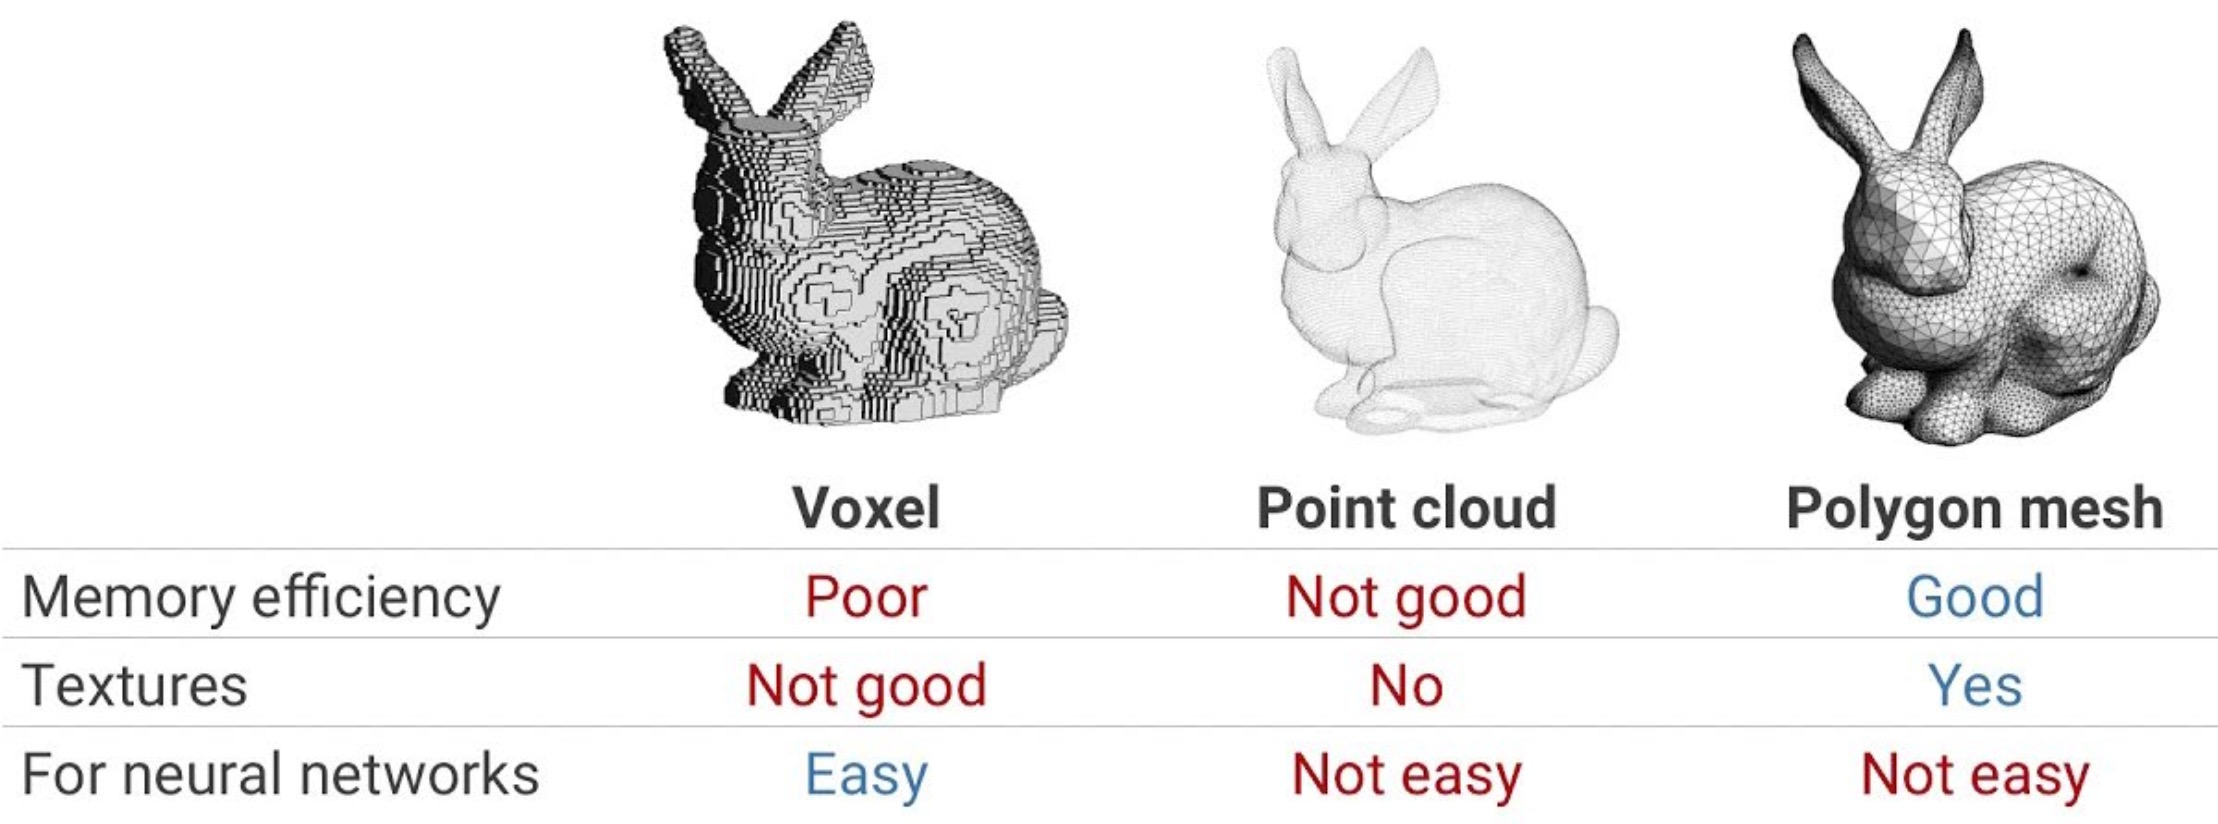
\includegraphics[width=\linewidth]{CV2-Latex-summary/Images/VoxelVSPCVSMesh.jpg}

\paragraph{Signed Distance Function (SDF; Implicit Surface)} An SDF is a function that maps a point in space to the signed-distance between the point and the nearest point on the object's surface. The set of all points with zero-SDF-values is called the \textit{isosurface} and represents the object surface. The sign represents whether points are in front of or behind the surface. We can extract a mesh from the isosurface using the \textit{Marching Cubes (MC) algorithm}. MC requires a voxel grid with SDF values as input and then places a mesh vertex whenever it registers a change in the sign between two voxels. There exist 15 possible isosurface configurations that can be extracted from a cube with 8 neighboring voxels.

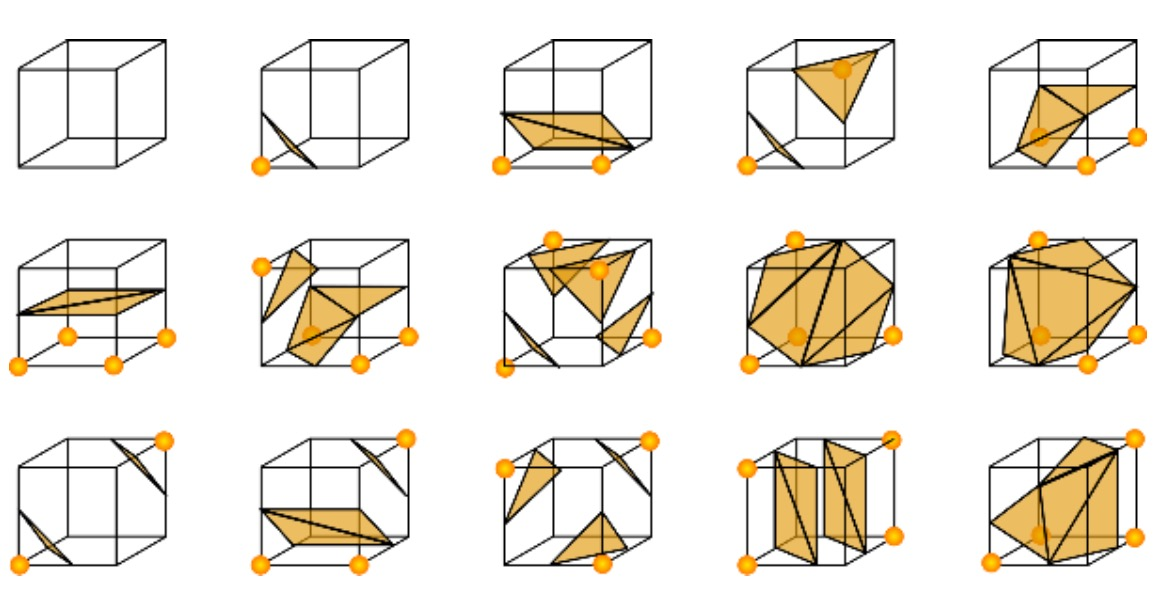
\includegraphics[width=\linewidth]{CV2-Latex-summary/Images/SDFVoxels.jpg}

\paragraph{``Line'' Cloud} The line features are more useful than points in a point cloud, but are also more difficult to extract under bad environment conditions. 

\paragraph{Integrated Information} In certain environments  additional information is available that we can \textit{integrate} into the scene representation. E.g.\ in urban environments we know that vertical lines are supposed to be parallel to each other and orthogonal to horizontal lines. In case of the facade of a house it may make sense to enforce co-planarity of all line for instance. We can also assign points class labels that we know from semantic segmentation.

\setlength{\columnsep}{0cm}
\begin{multicols}{3}
    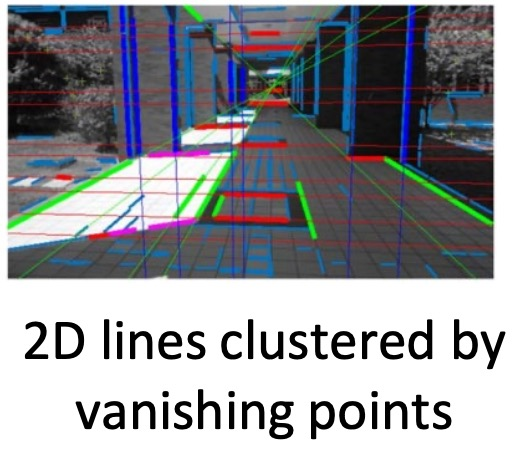
\includegraphics[width=\linewidth]{CV2-Latex-summary/Images/OrthogonalLines.jpg}
    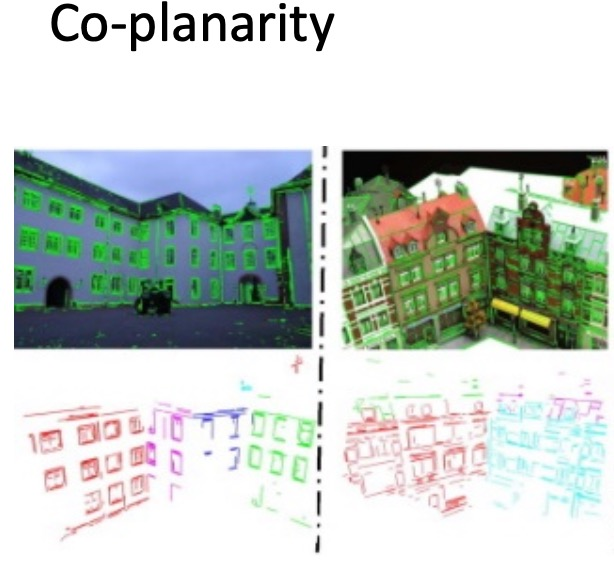
\includegraphics[width=\linewidth]{CV2-Latex-summary/Images/CoPlanar.jpg}
    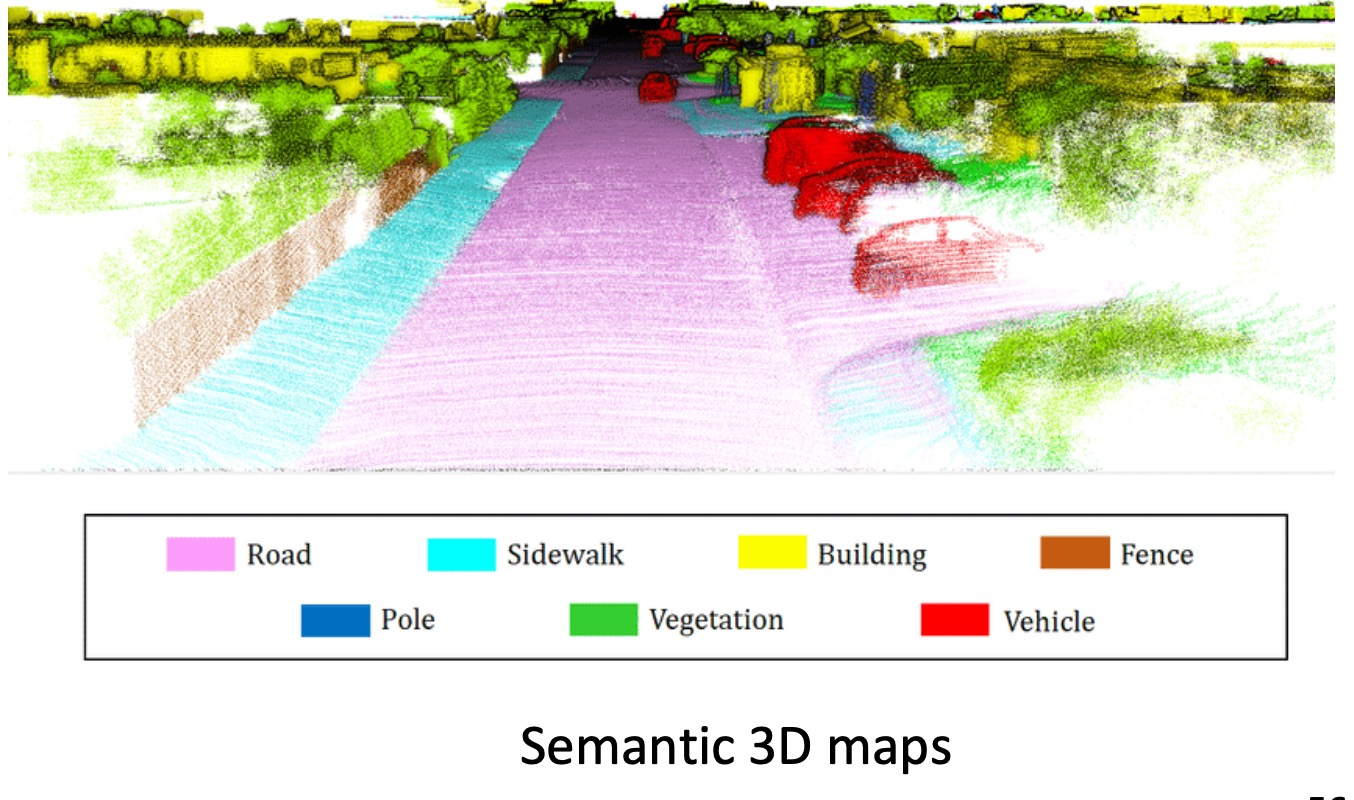
\includegraphics[width=\linewidth]{CV2-Latex-summary/Images/SemanticPC.jpg}
\end{multicols}

\end{multicols}

\newpage


%%%%%%%%%%%%%%%%%%%%%%%
%%% IMAGE FORMATION %%%
%%%%%%%%%%%%%%%%%%%%%%%


\begin{multicols}{2}[\section{Image Formation}]
\subsection{Ideal Perspective / Pinhole Camera}

\begin{myfigure}
    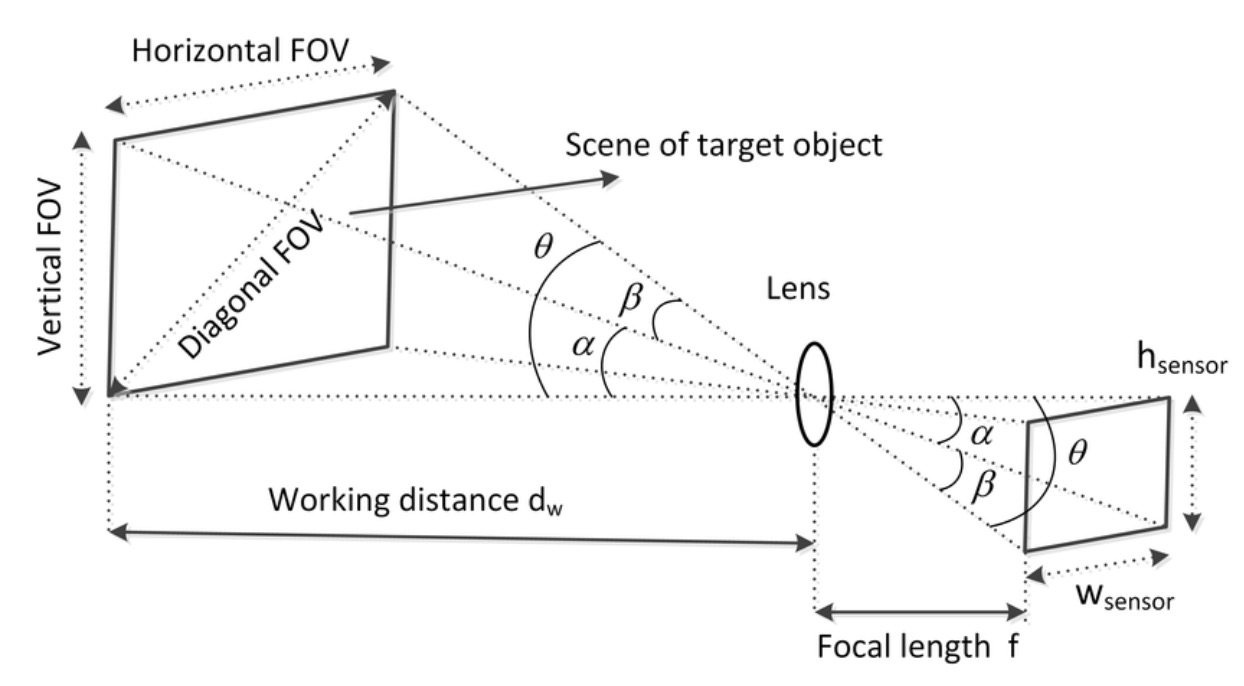
\includegraphics[width=\linewidth]{CV2-Latex-summary/Images/FOV.jpg}
\end{myfigure}


Perspective effects in perspective projections with the pinhole camera: 1) object size is inversely proportional to the distance; 2) parallel lines intersect at a \textit{vanishing point} where the connection between two horizontal vanishing points is the \textit{horizon}; 3) for convenience reasons, the \textit{virtual image plane} is placed in front of the lens, such that the image is not flipped.

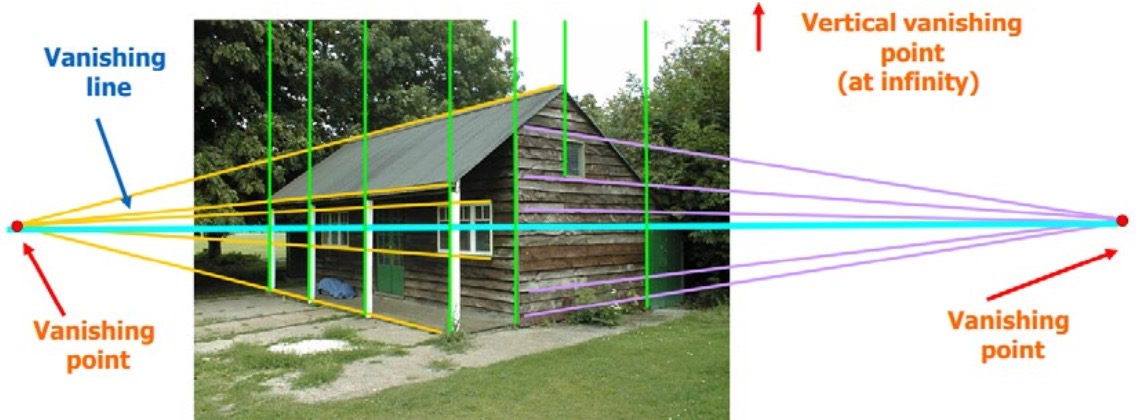
\includegraphics[width=\linewidth]{CV2-Latex-summary/Images/VanishingPoint.jpg}

The angles between the edges that span the viewing frustrum are called \textit{angle of view (AOV)} or \textit{FOV angle} and the extents of the scene at some target distance are called \textit{field of view (FOV)}:

\begin{flalign*}
    \text{AOV}&=2 \arctan\left(\frac{\text{sensor size}}{2f}\right)\quad\quad\text{[angle]}\\
    \text{FOV}&=2 \tan\left(\frac{\text{AOV}}{2}\right)\cdot d_w\quad\quad\text{[length]}
\end{flalign*}

\subsubsection{Intrinsic Camera Parameters} \label{subsection:intrinsic_parameters}

Pinhole camera model with the \textit{image plane} (informally referred to as the \textit{projection plane}) in front:
\begin{myfigure}
 \centering
 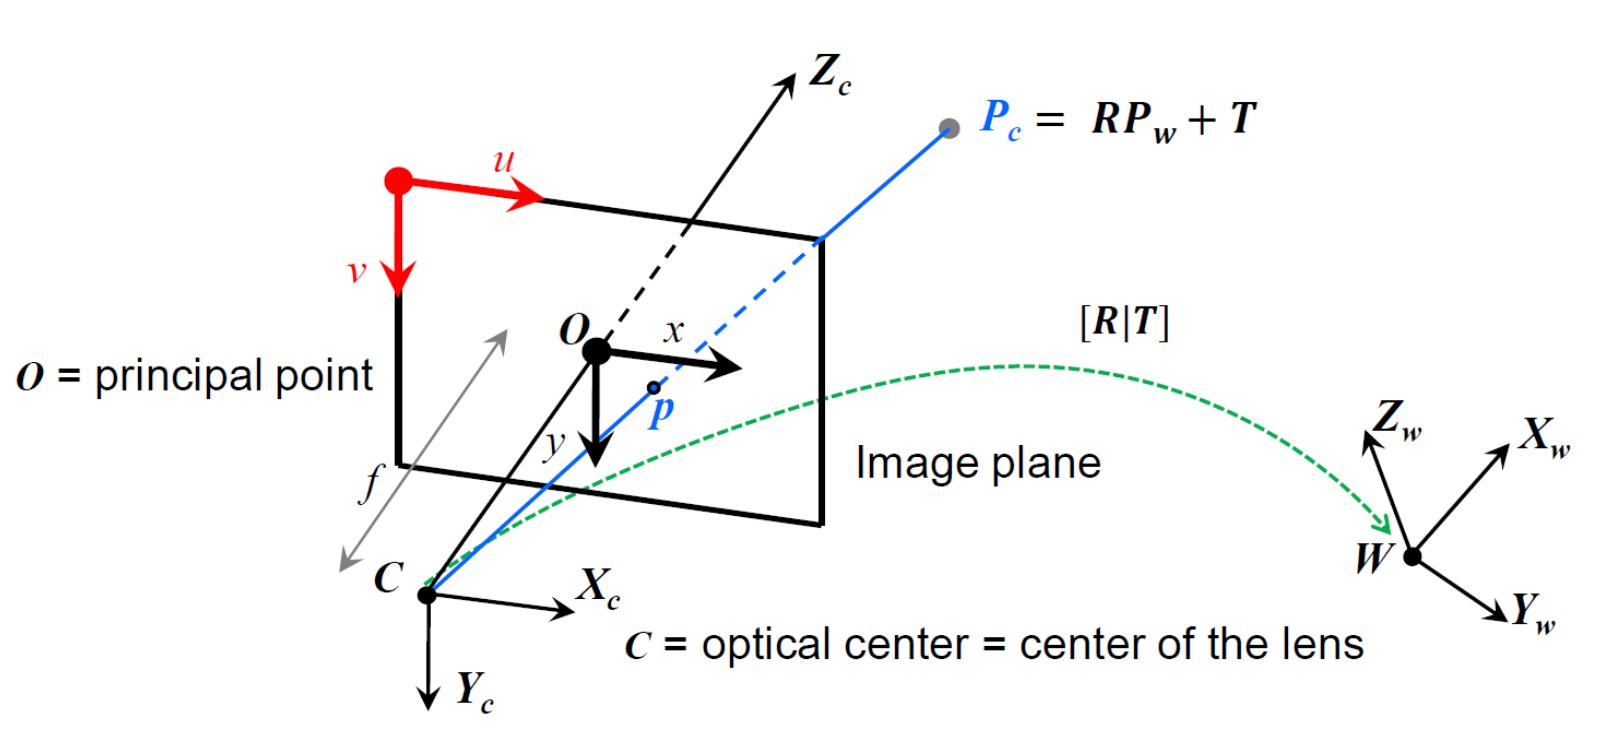
\includegraphics[width=1\linewidth]{CV2-Latex-summary/Images/PerspectiveProjection.jpg}
\end{myfigure}

The origin for image coordinates is in the center of the 2D image plane with expansion $(-1, -1)$ and $(1, 1)$.\\
The origin of pixel coordinates is moved to the bottom- or top-left corner to enable a purely positive expansion e.g. $(0, 0)$ and $(1024, 768)$. The \textbf{intrinsic/calibration camera matrix} $\mathbf{K}$ is:
\begin{equation*}
	\mathbf{K} = \mathbf{K}_s \mathbf{K}_f = \begin{psmallmatrix} s_x & s_{\theta} & o_x\\0 & s_y & o_y\\0 & 0 & 1\end{psmallmatrix}\begin{psmallmatrix} f & 0 & 0\\0 & f & 0\\0 & 0 & 1\end{psmallmatrix} = \begin{pmatrix}f s_x & f s_{\theta} & o_x\\0 & f s_y & o_y\\0 & 0 & 1 \end{pmatrix}
\end{equation*}
Its entries can be interpreted as follows:
\begin{itemize}
    \item $f$: focal length in [mm]
    \item $s_x$: scaling to pixels in x-direction [pixels/mm]
    \item $f\cdot s_x = \alpha_x$: unit length in x-direction [pixels]
    \item $s_y$: scaling to pixels in y-direction [pixels/mm]
    \item $f\cdot s_y = \alpha_y$: unit length in y-direction [pixels]
    \item $\alpha_x / \alpha_x$: aspect ratio $\sigma$
    \item $s_{\theta}$: skew factor for non-square pixels
    \item $f\cdot s_{\theta}$: skew of the pixel
    \item $o_x$: x-coordinate of principal point [pixels]
    \item $o_y$: y-coordinate of principal point [pixels]
\end{itemize}
For modern cameras, it it safe to assume $s_\theta=0$ and $\alpha_x=\alpha_y$. The \textbf{extrinsic camera matrix} describes the camera motion $g = \begin{pmatrix}\mathbf{R} & \mathbf{T}\\\mathbf{0}^T & 1 \end{pmatrix}$.


\subsection{Perspective Projection}

\paragraph{From Camera to Image Coordinates} The perspective transformation $\pi$ from camera coordinates $\boldsymbol{X}$ to image coordinates $x$ is given by
\begin{flalign*}
    &\pi : \mathbb{R}^3 \rightarrow \mathbb{R}^2; \quad \boldsymbol{X} \mapsto \mathbf{x} = \begin{psmallmatrix}x\\y\end{psmallmatrix} = \pi (\boldsymbol{X}) = \begin{pmatrix}\frac{X}{Z}\\ \frac{Y}{Z} \end{pmatrix}
    \\
    &\text{or in homogeneous coordinates;}
    \\
    &Z\boldsymbol{x} = Z\begin{psmallmatrix} x\\ y\\ 1 \end{psmallmatrix} = \mathbf{\Pi}_0 \boldsymbol{X}
					   = \begin{psmallmatrix} 1 & 0 & 0 & 0\\0 & 1 & 0 & 0\\0 & 0 & 1 & 0\end{psmallmatrix} \begin{psmallmatrix} X\\ Y\\ Z\\ 1 \end{psmallmatrix}	
\end{flalign*}

where $\mathbf{\Pi}_0$ is the standard projection matrix. We usually denote $Z$ as $\lambda = \text{const} > 0$ and multiply with the focal length to obtain image-space coordinates in [mm]:
\begin{equation*}
	\lambda \boldsymbol{x} = \mathbf{K}_f \Pi_0 \boldsymbol{X}.
\end{equation*}

\paragraph{From World to Image Coordinates} Transformation of point $\boldsymbol{X}_0$ in world coordinates to a point $\boldsymbol{X}$ in camera coordinates:
\begin{equation*}
	\boldsymbol{X} = g \boldsymbol{X}_0 = \begin{psmallmatrix} \mathbf{R} & \mathbf{T}\\\mathbf{0}^T & 1\end{psmallmatrix} \boldsymbol{X}_0.
\end{equation*}
Transformation from world coordinates to image coordinates:
\begin{equation*}
	\lambda \boldsymbol{x} = \mathbf{K}_f \mathbf{\Pi}_0 g \boldsymbol{X}_0.
\end{equation*}

\paragraph{To Pixel Coordinates} The pixel coordinates $\mathbf{x'}=(u\;v\;1)^T$ as a function of homogeneous camera coordinates $\boldsymbol{X}$ are given by
\begin{flalign*}
	&\lambda \boldsymbol{x}' = \lambda \begin{pmatrix} u\\v\\1 \end{pmatrix} = \mathbf{K}_s \mathbf{K}_f \mathbf{\Pi}_0 \boldsymbol{X} = \mathbf{K} \mathbf{\Pi}_0 \boldsymbol{X}
    \\
    &\text{which is equivalent to}\quad    \begin{pmatrix}u\\v\\1\end{pmatrix}=\begin{psmallmatrix}\frac{f s_x X}{Z}+o_x\\\frac{f s_y Y}{Z}+o_y\\1\end{psmallmatrix}
\end{flalign*}

and as function of world coordinates $\boldsymbol{X}_0$ by
\begin{equation*}
	\lambda \boldsymbol{x}' = \mathbf{K} \mathbf{\Pi}_0 \boldsymbol{X} = \mathbf{K} \mathbf{\Pi}_0 g \boldsymbol{X}_0 \equiv \mathbf{\Pi} \boldsymbol{X}_0.
\end{equation*}
The matrix $\mathbf{\Pi} \equiv \mathbf{K} \mathbf{\Pi}_0 g = (KR,KT)$ is the general projection matrix.

\paragraph{Summary for Homogeneous Coordinates:} 4D world coordinates $\boldsymbol{X}_0$ $\xrightarrow{g \, \in \, SE(3)}$ 4D camera coordinates $\boldsymbol{X}$ $\xrightarrow{\mathbf{K}_f \mathbf{\Pi}_0}$ 3D image coordinates $\boldsymbol{x}$ in [mm] $\xrightarrow{\mathbf{K}_s}$ 3D pixel coordinates $\boldsymbol{x'}$.

\paragraph{Normalized Image Plane} In order to interpret image-space features as camera-space features (e.g.\ a 2D point as a 3D point), we construct a virtual image plane with $f=1$ and the origin of the pixel coordinates at the principal point.
\begin{myfigure}
    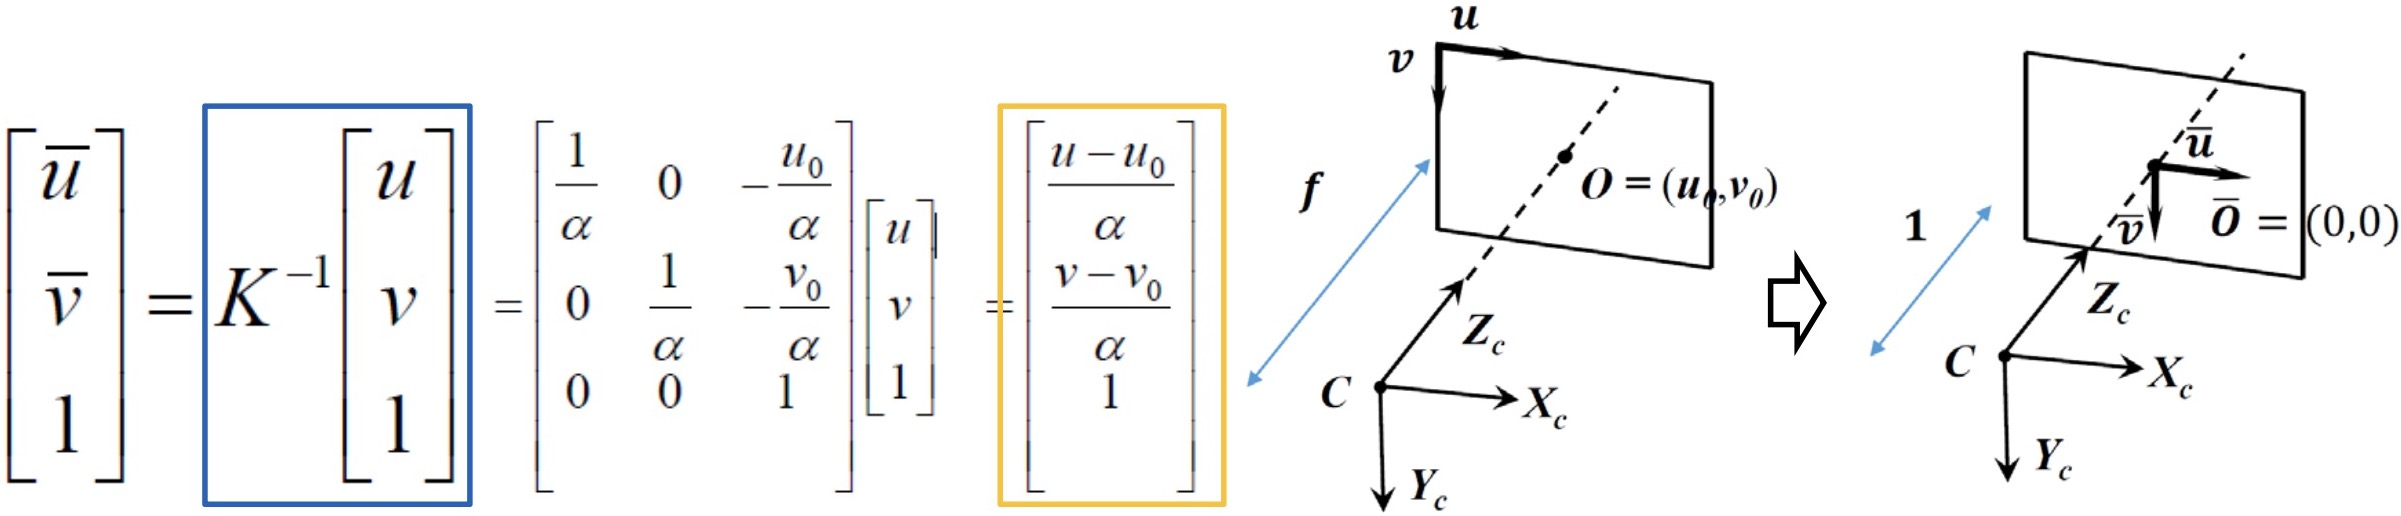
\includegraphics[width=\linewidth]{CV2-Latex-summary/Images/NormalizedImagePlane.jpg}
\end{myfigure}

\paragraph{Comparison to Computer Graphics} The main difference that in CG, we transform the viewed volume, i.e.\ the pyramidal frustum in front of the image, into a unit cube that is described by normalized device coordinates (NDC; $\in[-1,1]$). Mathematically, we project a camera-space point $\mathbf{x}_\text{eye}$ into the \textit{NDC-space} via:
\begin{flalign*}
    &\begin{psmallmatrix}x_\text{clip}\\y_\text{clip}\\z_\text{clip}\\w_\text{clip}\end{psmallmatrix}
    = \underbrace{\begin{psmallmatrix}
        \frac{2n}{r-l} & 0 & -\frac{r+l}{r-l} & 0 \\
        0 & \frac{2n}{t-b} & -\frac{t+b}{t-b} & 0 \\
        0 & 0 & \frac{f+n}{f-n} & -\frac{2fn}{f-n} \\
        0 & 0 & 1 & 0
    \end{psmallmatrix}}_{\text{Perspective matrix }\mathbf{P}}
    \begin{psmallmatrix}x_\text{eye}\\y_\text{eye}\\z_\text{eye}\\w_\text{eye}\end{psmallmatrix}
    \\
    &\text{such that}\quad \begin{psmallmatrix}x_\text{ndc}\\y_\text{ndc}\\z_\text{ndc}\end{psmallmatrix}=\begin{psmallmatrix}x_\text{clip}/w_\text{clip}\\y_\text{clip}/w_\text{clip}\\z_\text{clip}/w_\text{clip}\end{psmallmatrix}
\end{flalign*}
\begin{myfigure}
    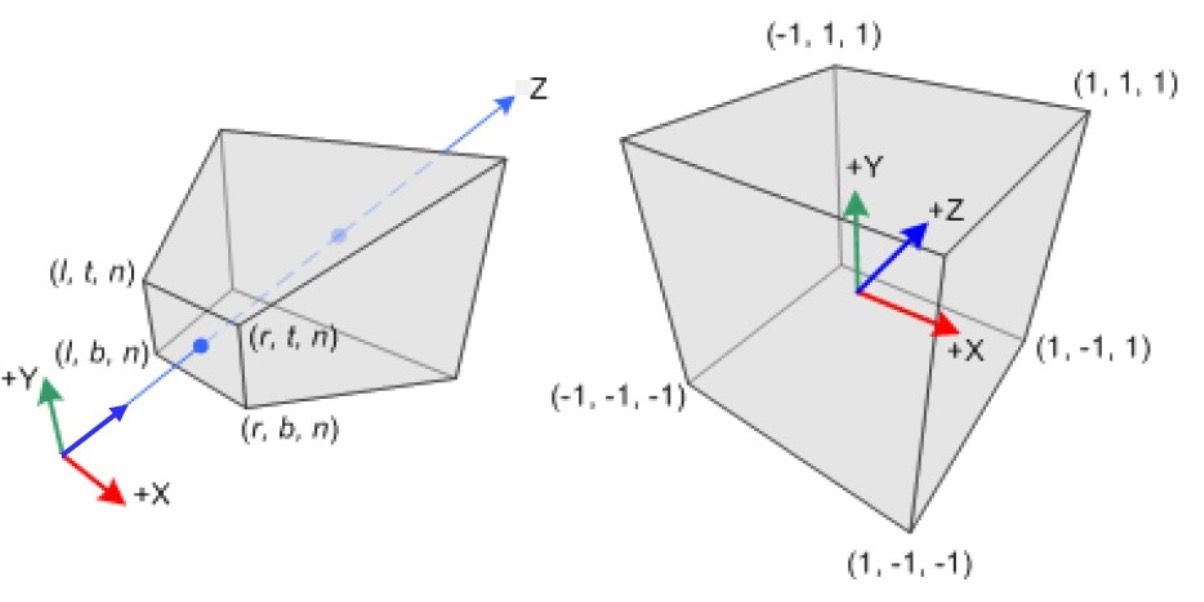
\includegraphics[width=\linewidth]{CV2-Latex-summary/Images/NDCSpace.jpg}
\end{myfigure}
In contrast to CV, every projected point $\mathbf{x}_\text{ndc}$ retains normalized depth information. We get \textit{image space} coordinates by projecting the NDC space onto the XOY-plane and stretching it to the screen width and height.

\paragraph{Line Projection} Naively, we project a line into image space by projecting each of its endpoints. The \textit{intrinsic matrix for line projection} $\mathbf{\mathcal{K}}$ allows a one-step computation of the line coordinates :
\begin{flalign*}
    \mathbf{l}=\mathbf{\mathcal{K}}\mathbf{n}
    \quad\text{with}\quad
    \mathbf{\mathcal{K}}=\begin{psmallmatrix}f_y&0&0\\0&f_x&0\\-f_y x_0&-f_x y_0&f_x f_y\end{psmallmatrix}
\end{flalign*}
where $\mathbf{n}$ is the normal of the \textbf{projection plane} of the line according to its Plücker coordinates and the 2D line $\mathbf{l}$ is defined as:

\begin{flalign*}
     ax+by+c = 0\quad\text{with }\mathbf{l}=\begin{pmatrix}a\\b\\c\end{pmatrix}
     = \underbrace{\begin{psmallmatrix}x_0\\y_0\\1\end{psmallmatrix} \times \begin{psmallmatrix}x_1\\y_1\\1\end{psmallmatrix}}_{\text{two points}}
\end{flalign*}

We can calculate it from the cross product of the vectors from the principal points to the line's image-space end-points.
\begin{myfigure}
    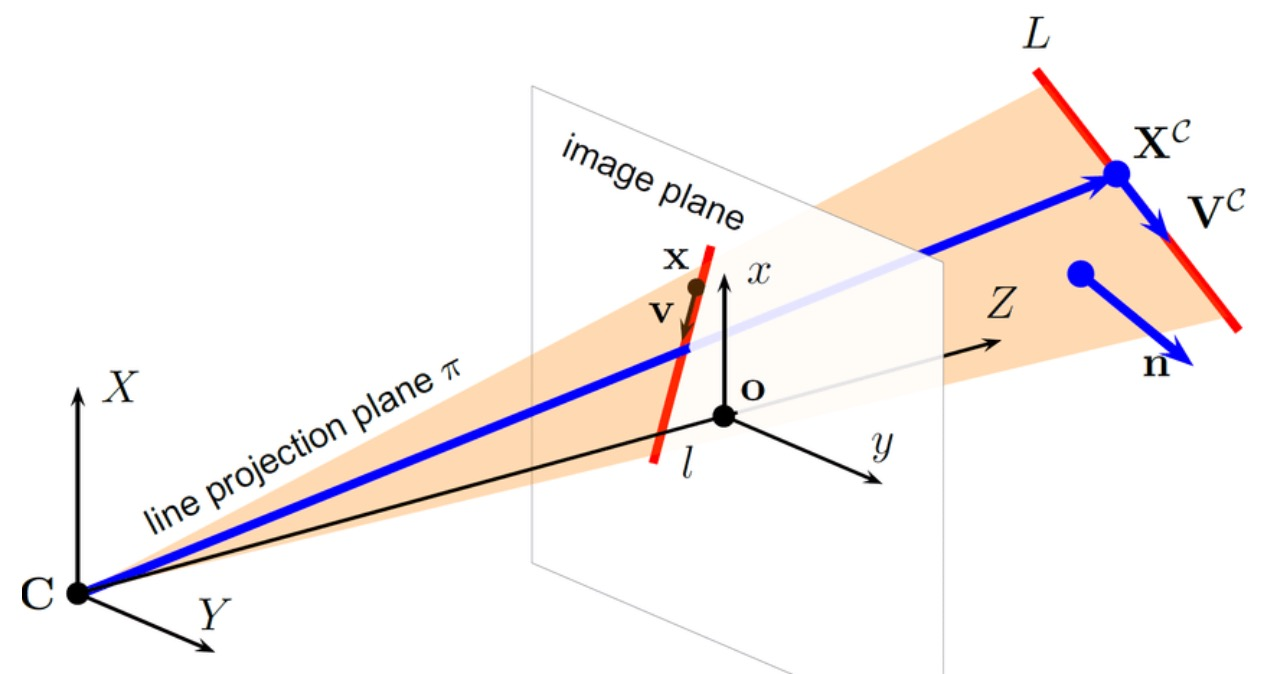
\includegraphics[width=0.8\linewidth]{CV2-Latex-summary/Images/LineProjection.jpg}
\end{myfigure}
An image-space line $\mathbf{l}$ corresponds to a world-space line $\mathbf{L}$ if their projection-plane-normals are parallel (\textit
line constraint):
\begin{flalign*}
    \mathbf{n}^\mathbf{l}\propto \mathbf{n}^\mathbf{L} \quad\Rightarrow\quad \mathbf{\mathcal{K}}^{-1}\mathbf{l} \propto [\mathbf{R} [\mathbf{t}]_\times \; \mathbf{R}]\mathbf{L}
\end{flalign*}

Two parallel vectors have a cross product of zero. Because a $3\times3$ skew-symmetric matrix has rank 3, this parallelism of each 3D-2D line correspondence provides two constraints.

\begin{multicols}{2}
    All 3D vectors in a projection plane are projected onto the same 2D line which is known as the \textbf{projection ambiguity problem}. $L_1, L_2, L_3$ share the same normal $\mathbf{n}$ up to a scalar factor, which is irrelevant when computing $\mathbf{l}=\mathbf{\mathcal{K}}\mathbf{n}$. We say, the projections are \textit{identical up-to-scale}.
    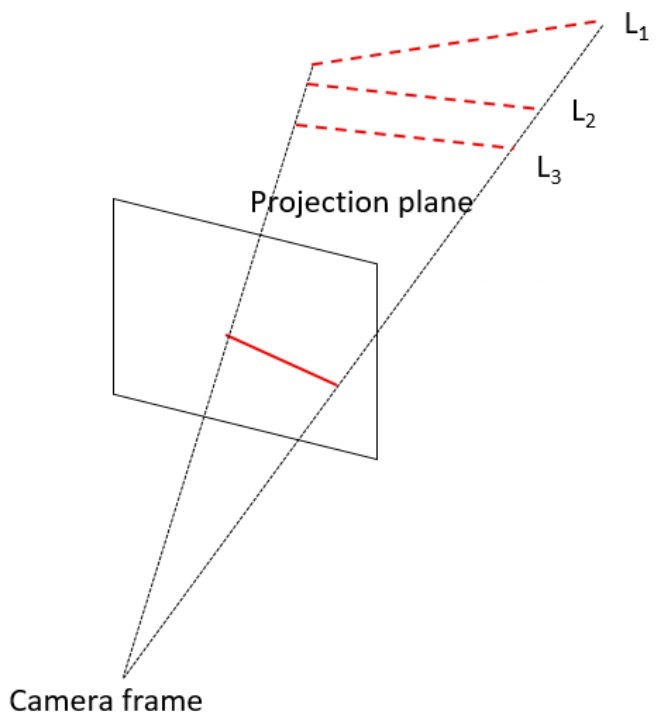
\includegraphics[width=\linewidth]{CV2-Latex-summary/Images/AmbiguityProblem.jpg}
\end{multicols}

\paragraph{Relationship between Points, Lines and Planes} We describe a \textbf{3D plane} using a four-dim.\ vector $(A\;B\;C\;D)^T$, where the first three coordinates are the normal and $D$ is the projected distance from the origin. These coordinates must satisfy the constraint $Ax+By+Cz=D$. A \textbf{3D point} $\mathbf{P}=(X\;Y\;Z\;1)^T$ lies on a plane if $\mathbf{P}^T \mathbf{n}=0$ holds.

\begin{multicols}{2}
    {
    The projection plane of an image-space line $\mathbf{l}_L$ is:
    $$\underbrace{\mathbf{\pi_L}}_{4\times1}=\underbrace{\mathbf{P}^T}_{\substack{(3\times4)^T\text{}\\ \text{Proj.\ matrix}}} \underbrace{\mathbf{l}_L}_{3\times1} \in \mathbb{R}^4$$

    The intersection between a 3D line $\mathcal{L}=(\mathbf{n}, \mathbf{v})$ and 3D plane $\mathbf{\pi}$ is:
    $$\mathbf{D}=\mathbf{L}\mathbf{\pi} \quad\text{with}\quad \mathbf{L}=\begin{psmallmatrix}[\mathbf{n}]_\times & \mathbf{v} \\ -\mathbf{v}^T & 0\end{psmallmatrix}$$
    }
    \hfill
    \begin{center}
        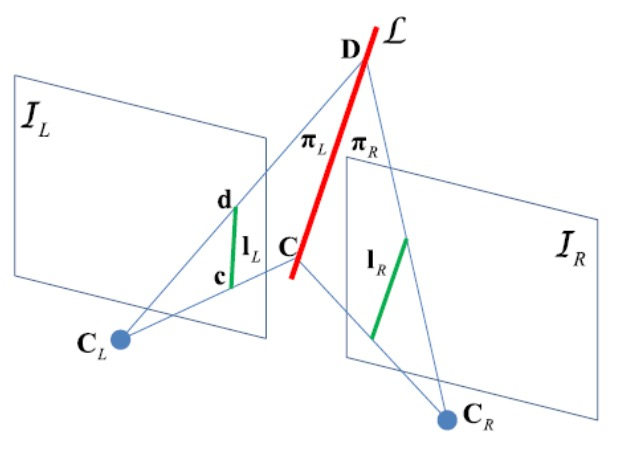
\includegraphics[width=4cm]{CV2-Latex-summary/Images/LineProjectionPlane.jpg}
        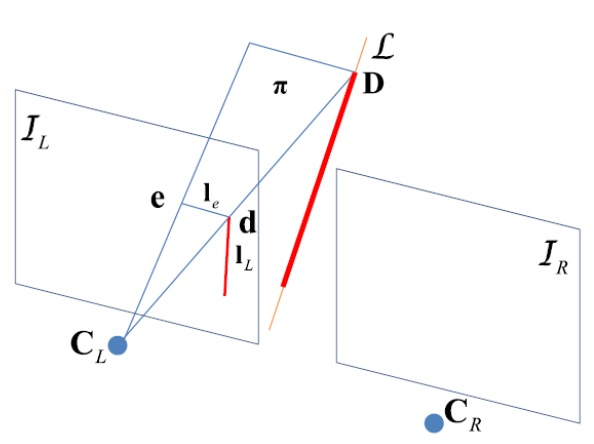
\includegraphics[width=3cm]{CV2-Latex-summary/Images/LinePlaneIntersection.jpg}
    \end{center}
\end{multicols}
An image-space point $\mathbf{x}$ corresponds to a world space point $\mathbf{X}$, if their ray direction vectors $\mathbf{d}$ (starting from the principal point) are parallel (\textit{point constraint}):
\begin{flalign*}
    \mathbf{d}^\mathbf{x}\propto \mathbf{d}^\mathbf{X} \quad\Rightarrow\quad \mathbf{\mathcal{K}}^{-1}\mathbf{x} \propto [\mathbf{R} \; \mathbf{t}]\mathbf{X}
\end{flalign*}


\subsection{Parallel Projection}

Whereas the perpective projection looks realistic, since object size changes inversely with the distance, the parallel projection is better to obtain exact measurements of objects. That is because parallel 3D lines remain parallel in the 3D projection, since the viewing frustrum has the shape of a cuboid.

\begin{wrapfigure}{r}{0.4\linewidth}
    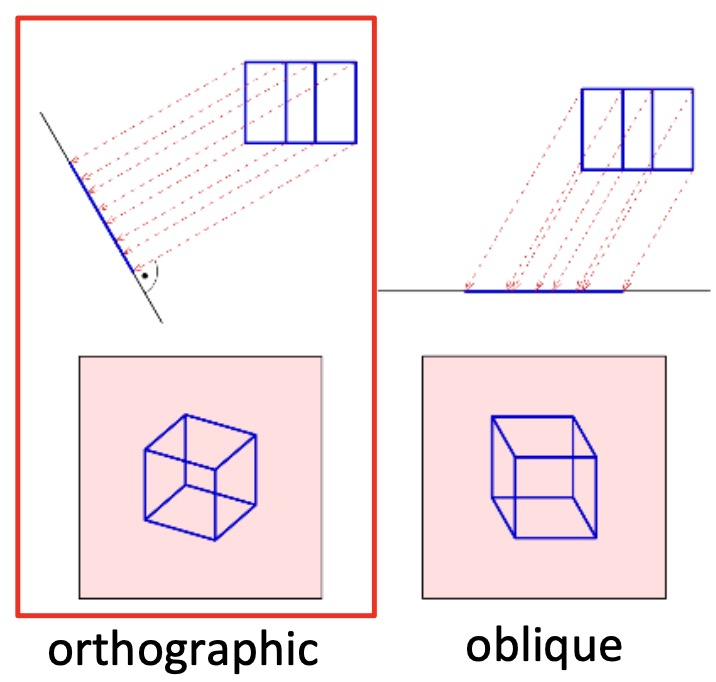
\includegraphics[width=\linewidth]{CV2-Latex-summary/Images/ParallelProjections.jpg}
\end{wrapfigure}

\paragraph{Orthographic Projection} This is a special case where the projection rays are perpendicular to the projection plane. We use this projection to projection 3D points into a birds-eye-view of the scene, which is useful in robotics applications.

\paragraph{Oblique Projection} The projection rays intersect with the image plane at a skew angle. 

\subsection{Spherical Projection}
Instead of a planar projection surface, one can consider a spherical projection surface given by the unit sphere $\mathbb{S}^2 = \{\mathbf{x} \in \mathbb{R}^3 \ \vert \ \norm{\mathbf{x}}=1\}$.
The spherical projection $\pi_s$ of a 3D point $\boldsymbol{X}$ is given by:
\begin{equation*}
    \pi_s: \mathbb{R}^3 \rightarrow \mathbb{S}^2; \quad \boldsymbol{X} \mapsto \boldsymbol{x} = \frac{\boldsymbol{X}}{|\boldsymbol{X}|}
\end{equation*}
Next, we convert our Cartesian coordinates $\mathbf{x}$ to spherical coordinates azimuth $\theta=\arctan(\frac{y}{x})\in[0,2\pi)$ and the polar angle $\phi=\arccos(\frac{z}{r})\in[0,\pi]$ with $r=\sqrt{x^2+y^2+z^2}=1$ for a unit sphere. We get the image space coordinates by linearly mapping the spherical coordinates onto a 2D plane.
\begin{equation*}
    x = r\cos\theta\sin\phi 
    \quad\quad
    x = r\sin\theta\sin\phi 
    \quad\quad
    z = r\cos\phi
\end{equation*}

\begin{myfigure}
    % 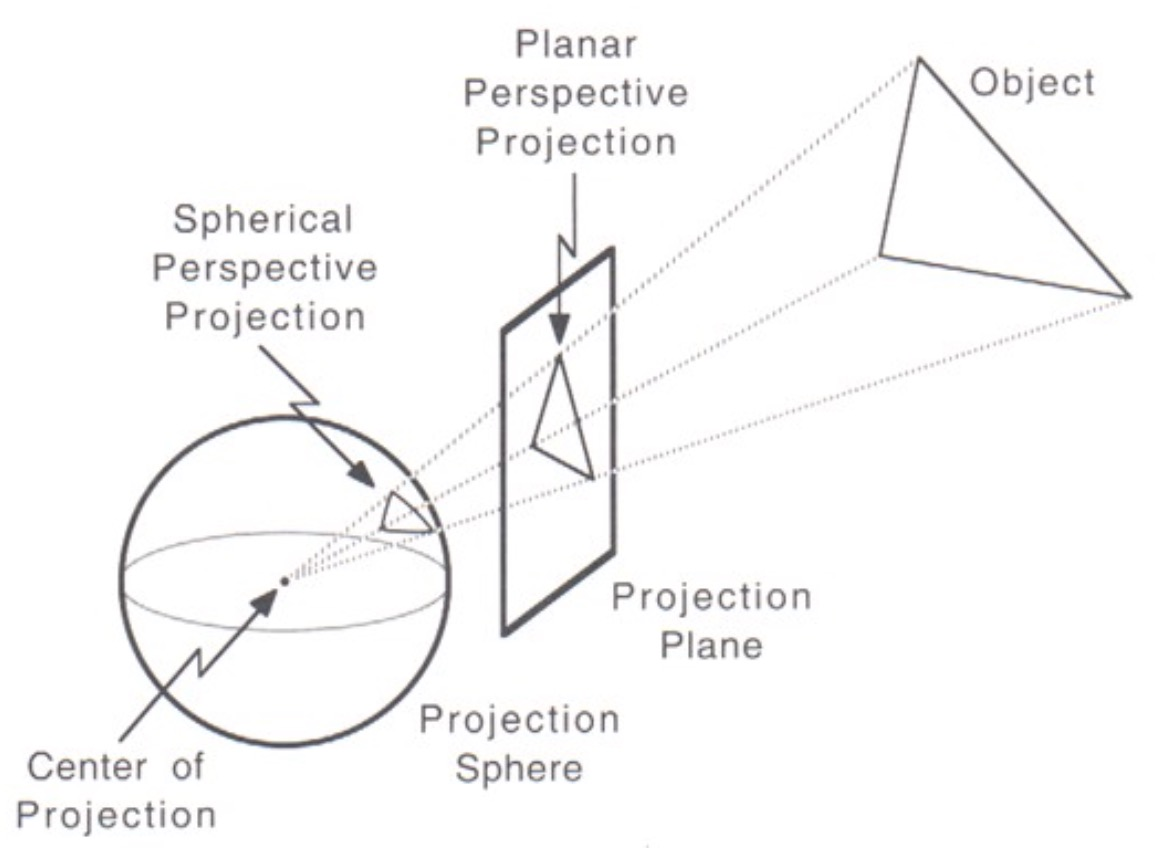
\includegraphics[width=\linewidth/3]{CV2-Latex-summary/Images/SphericalProjection.jpg}
    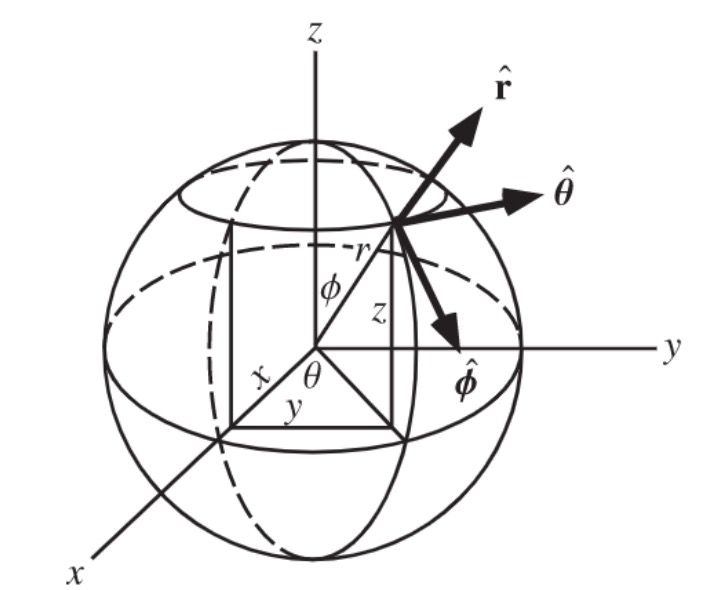
\includegraphics[width=0.4\linewidth]{CV2-Latex-summary/Images/SphericalCoordinates.jpg}
    \hfill
    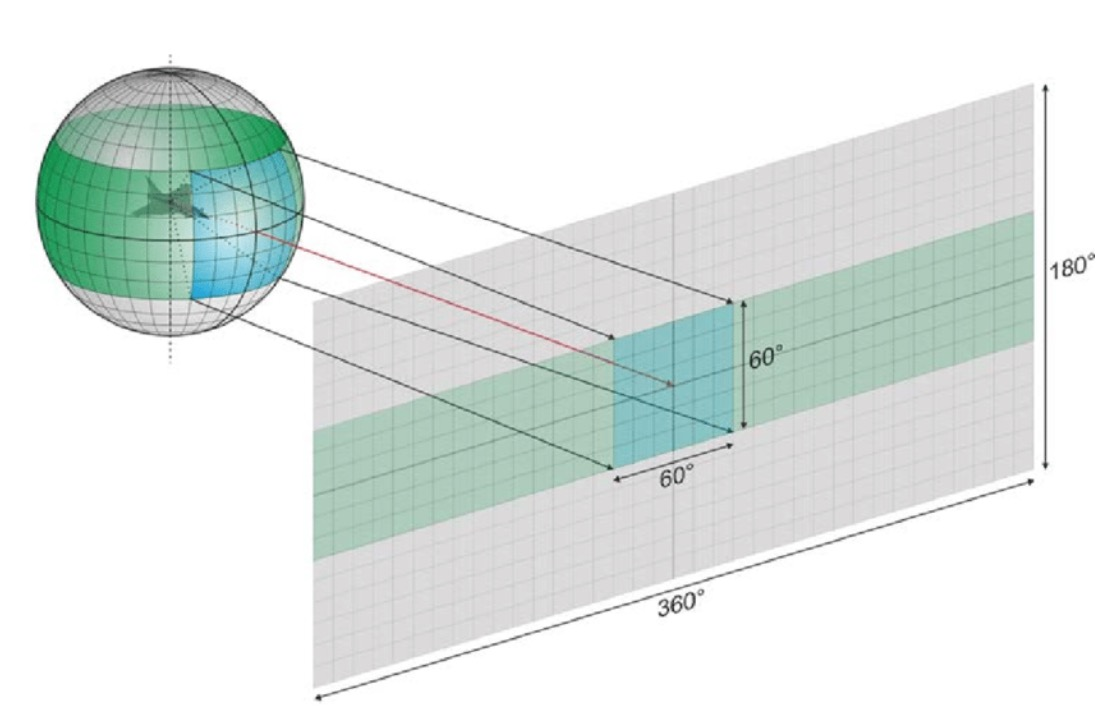
\includegraphics[width=0.49\linewidth]{CV2-Latex-summary/Images/UwrapSphere.jpg}
\end{myfigure}

The whole projection equation becomes:
\begin{equation*}
    \lambda \boldsymbol{x}' = K \Pi_0 g \boldsymbol{X}_0
\end{equation*}
is similar to the previous one except for $\lambda = \norm{\boldsymbol{X}} = \sqrt{X^2 + Y^2 + Z^2}$.

\paragraph{Other Expressions of a Sphere} We obtain an \textit{icosahedral spherical representation} by extruding all the vertices of icosahedron sub-faces to the unit sphere.
\begin{center}
    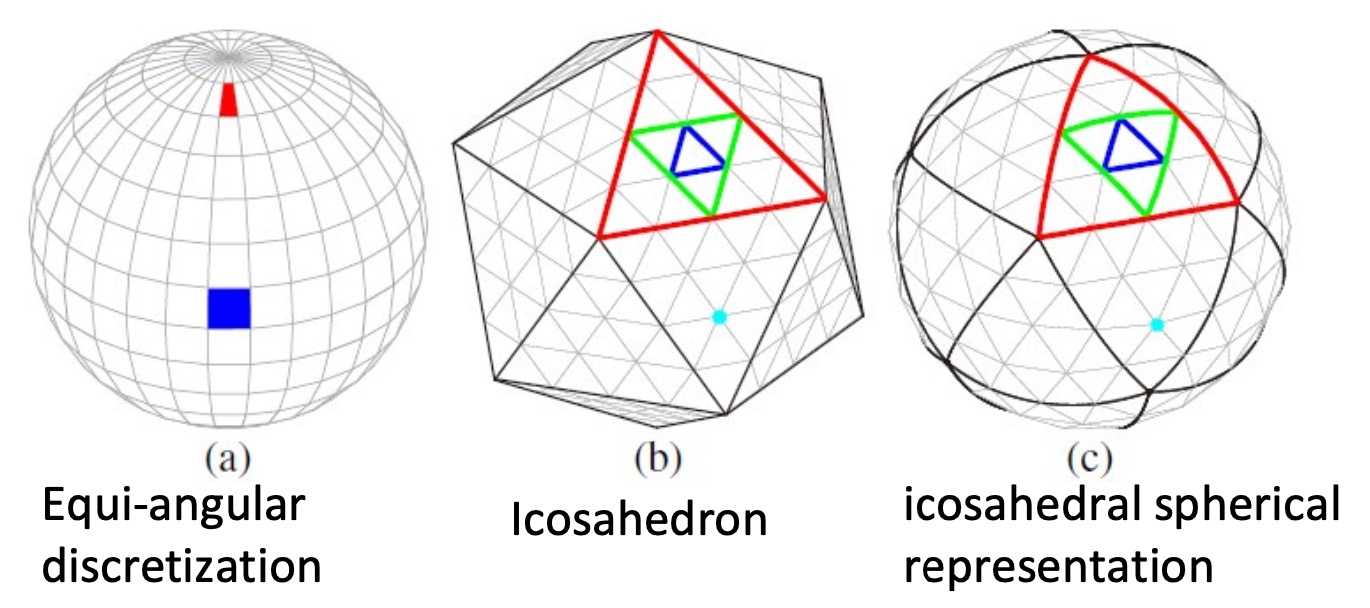
\includegraphics[width=\linewidth]{CV2-Latex-summary/Images/SphereRepresentations.jpg}
\end{center}

\subsection{Distortion}

\begin{wrapfigure}{r}{0.3\linewidth}
    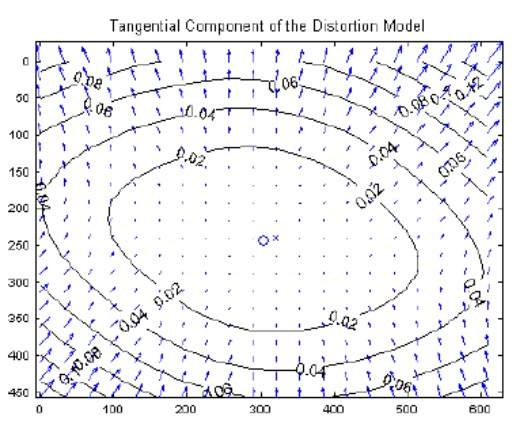
\includegraphics[width=\linewidth]{CV2-Latex-summary/Images/TangentialDistortion.jpg}
\end{wrapfigure}
\textbf{Tangential distortion} happens if lens and image sensor are not perfectly parallel. The projected image will appear stretched/staunched in certain directions.

\paragraph{Radial Distortion} This occurs, when light rays bend more at the lens' edges than at its optical center. 
\begin{myfigure}
    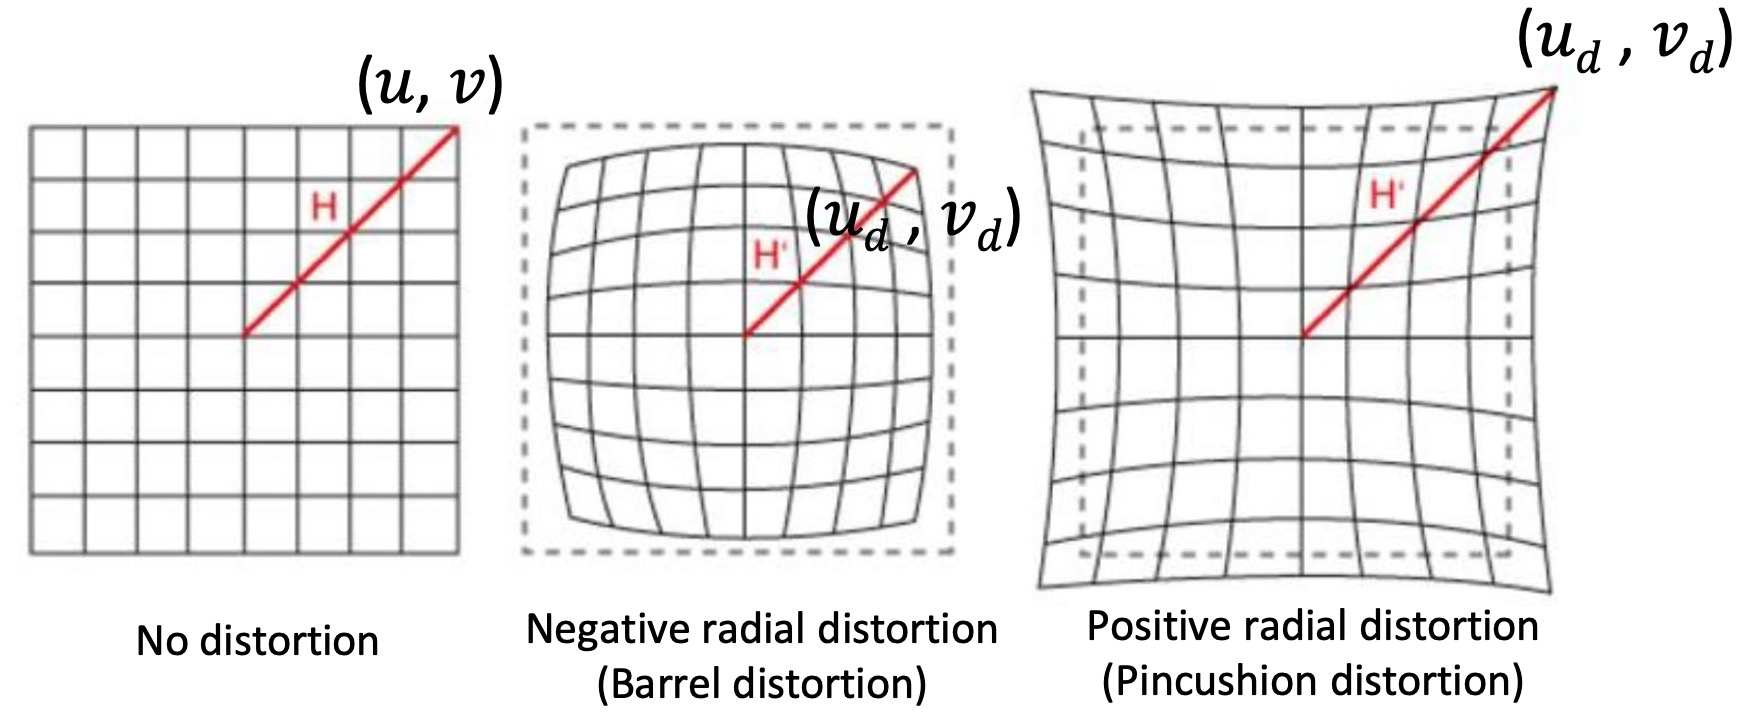
\includegraphics[width=\linewidth]{CV2-Latex-summary/Images/RadialDistortion.jpg}
\end{myfigure}
In simple quadratic model of radial distortion, we calculate the distorted coordinates $\boldsymbol{x}'_d$ from (ideal) non-distorted coordinates $\boldsymbol{x}'$:
{\small\begin{flalign*}
    \begin{pmatrix}u_d\\v_d\end{pmatrix} = (1 + k_1 r^2) \begin{pmatrix}u-u_0\\v-v_0\end{pmatrix} + \begin{pmatrix}u_0\\v_0\end{pmatrix}
    \quad\text{with } \begin{aligned}
        r^2 =\ &(u-u_0)^2 +
        \\& (v-v_0)^2
    \end{aligned}
\end{flalign*}}
where $r$ is the radius and $k_1$ is a parameter estimated during calibration. \\
A more general model with an arbitrary center of distortion $\mathbf{c}$ is
\begin{equation*}
    \boldsymbol{x} = \mathbf{c} + f(r)(\boldsymbol{x}_d - \mathbf{c}) \quad \text{with} \quad r = |\boldsymbol{x}_d - \mathbf{c}| 
\end{equation*}
\begin{equation*}
    \text{and} \quad f(r) = 1 + a_1r+a_2r^2+a_3r^3 + a_4 r^4.
\end{equation*}

\subsection{Preimage and Coimage [old]}
Due to the unknown scale factor, each point is mapped not to a single point $\boldsymbol{x}$, but to an equivalence class of points $\boldsymbol{y} \sim \boldsymbol{x}$.
\begin{myfigure}
	\centering
	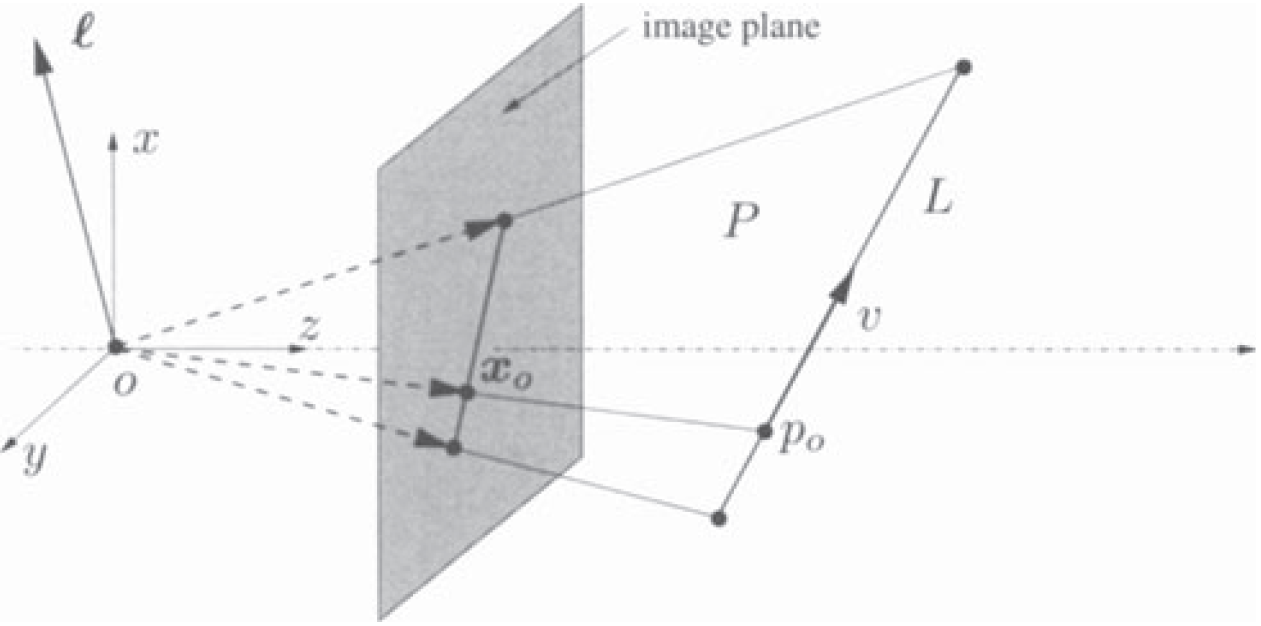
\includegraphics[width=0.8\linewidth]{Images/preimage.PNG}
\end{myfigure}
A line $L$ in 3D is characterized by a base point $\boldsymbol{X}_0 = (X_0, Y_0, Z_0, 1)^T \in \mathbb{R}^4$ and a vector $\boldsymbol{V} = (V_1, V_2, V_3, 0)^T \in \mathbb{R}^4$:
\begin{equation*}
    \boldsymbol{X} = \boldsymbol{X}_0 + \mu \boldsymbol{V} \subset \mathbb{R}^4, \quad \mu \in \mathbb{R}
\end{equation*}
The image of the line $L$ is given by
\begin{equation*}
    \boldsymbol{x} \sim \Pi_0 \boldsymbol{X} = \Pi_0(\boldsymbol{X}_0 + \mu \boldsymbol{V}) = \Pi_0 \boldsymbol{X}_0 + \mu \Pi_0 \boldsymbol{V}
\end{equation*}
All points $\boldsymbol{x}$ treated as vectors from the origin $o$ span a 2D subspace $P$.
The intersection of this plane $P$ with the image plane gives the image of the line.
$P$ is called the preimage of the line.\\
A preimage of a point or a line in the image plane is the largest
set of 3D points that give rise to an image equal to the given
point or line.\par
\vspace{11pt}
The coimage of a point or a line is the subspace in $\mathbb{R}^3$ that is the unique orthogonal complement, i.e. the normal vector, of its preimage.
Image, preimage and coimage are equivalent.\par

In the case of a line $L$ with its 2D preimage, we have
\begin{equation*}
    \boldsymbol{\ell}^T \boldsymbol{x} = 0 \text{  and  } P = \text{span}(\hat{\boldsymbol{\ell}}).
\end{equation*}
$\boldsymbol{\ell} \in \mathbb{R}^3$ is the normal vector to the preimage (2D subspace) of line $L$ and $\text{span}(\hat{\boldsymbol{\ell}})$ is the span of row vectors of $\hat{\boldsymbol{\ell}}$.

\vspace{1mm}
\renewcommand{\arraystretch}{1.3}%
\begin{tabularx}{\linewidth}{|c|Y|Y|Y|}
    \hline
     & Image & Preimage & Coimage \\ \hline
     Point & $\text{span}(\boldsymbol{x}) \, \cap \text{im. plane}$ & $\text{span}(\boldsymbol{x}) \subset \mathbb{R}^3$ & $\text{span}(\hat{\boldsymbol{x}}) \subset \mathbb{R}^3$ \\ \hline
     Line & $\text{span}(\hat{\boldsymbol{\ell}}) \, \cap \text{im. plane}$ & $\text{span}(\hat{\boldsymbol{\ell}}) \subset \mathbb{R}^3$ & $\text{span}(\boldsymbol{\ell}) \subset \mathbb{R}^3$ \\ \hline
\end{tabularx}
\renewcommand{\arraystretch}{1.0}%

\subsection{Projective Geometry}
One can represent 3D points by a general 4D vector $X = (XW, YW, ZW, W) \in \mathbb{R}^4$ remembering that only the direction of this vector is of importance.
We therefore identify the point in homogeneous coordinates with the line connecting it with the origin.

\subsection{Supplementary Knowledge}
\paragraph{Depth of Field} This is the distance between the nearest an farthest objects in a scene that appear acceptably sharp in an image. A narrower aperture increases the depth of field, but reduces the exposure of the image (darker).

\paragraph{Depth Camera} A camera that estimates the depth of each pixel by measuring the return time of each light ray (\textit{time-of-flight} measurement principle).

\paragraph{Rolling/Global Shutter Camera} With a rolling shutter, every row/pixel in the image is read on after the other at different times. This may cause distortions for moving objects. A global shutter exposes and reads all pixels simultaneously. When two images are recorded with rolling shutters that use different read-out directions (such that the motion-induced distortion is different), we can recover the motion and undistorted image from point correspondences.

\paragraph{Event Camera} Each pixel inside an event camera operates independently and asynchronously, reporting changes in brightness as they occur, and staying silent otherwise. We use this to improve robustness, efficiency and accuracy in visual odometry.

\end{multicols}
\newpage

% #############################
% #### CAMERA CALIBRATION #####
% #############################

\begin{multicols}{2}[\section{Camera Calibration}]

Camera calibration is the process of \textit{simultaneously} determining the extrinsic parameters $(\mathbf{R}, \mathbf{t})$ and intrinsic parameters $\mathbf{K}$, plus the lens distortion. In general, we estimate the intrinsic parameters first and subsequently obtain the extrinsic parameters from VO/SLAM.

\subsection{Tsai's Method}
We measure the 3D position of at least 6 3D control points on a calibration target, as well as their 2D projected coordinates. This methods uses a single image. We need to solve for the coefficients in the linear mapping from 3D world coordinates $\mathbf{p}$ to homogeneous pixel coordinates using the \textit{direct linear transform (DLT)}:

\begin{flalign*}
    \lambda\begin{psmallmatrix}u \\v \\1 \end{psmallmatrix}=\underbrace{
    \begin{psmallmatrix}
    \alpha_u & 0 & u_0 \\
    0 & \alpha_v & v_0 \\
    0 & 0 & 1
    \end{psmallmatrix}\begin{psmallmatrix}
    r_{11} & r_{12} & r_{13} & t_1 \\
    r_{21} & r_{22} & r_{23} & t_2 \\
    r_{31} & r_{32} & r_{33} & t_3
    \end{psmallmatrix}}_{
    = \mathbf{M}\;\in\;\mathbb{R}^{3\times4}
    } \underbrace{\begin{pmatrix}X_w \\Y_w \\Z_w \\1\end{pmatrix}}_{=\mathbf{p}}
    = \begin{psmallmatrix}\mathbf{m}^T_1\\\mathbf{m}^T_2\\\mathbf{m}^T_3\end{psmallmatrix}\mathbf{p}
\end{flalign*}

Conversion to non-homogeneous pixel coordinates leads to a system of linear equations with the values of $\mathbf{M}$ as coefficients:

\begin{flalign*}
    \begin{aligned}
    & u=\frac{\lambda u}{\lambda}=\frac{\mathbf{m}_1^{\mathrm{T}} \cdot \mathbf{p}}{\mathbf{m}_3^{\mathrm{T}} \cdot \mathbf{p}} \\
    & v=\frac{\lambda v}{\lambda}=\frac{\mathbf{m}_2^{\mathrm{T}} \cdot \mathbf{p}}{\mathbf{m}_3^{\mathrm{T}} \cdot \mathbf{p}}
    \end{aligned} 
    \quad\Rightarrow \underbrace{\substack{
    \left(\mathbf{m}_1^{\mathrm{T}}-u \mathbf{m}_3^{\mathrm{T}}\right) \cdot \mathbf{p}=0 \\
    \left(\mathbf{m}_2^{\mathrm{T}}-v \mathbf{m}_3^{\mathrm{T}}\right) \cdot \mathbf{p}=0}
    }_{=\underbrace{\begin{psmallmatrix}
    \mathbf{p}^{\mathrm{T}} & \mathbf{0}^{\mathrm{T}} & -u \mathbf{p}^{\mathrm{T}} \\
    \mathbf{0}^{\mathrm{T}} & \mathbf{p}^{\mathrm{T}} & -v \mathbf{p}^{\mathrm{T}}
    \end{psmallmatrix}}_{\mathbf{Q}}
    \begin{psmallmatrix}\mathbf{m}_1 \\\mathbf{m}_2 \\\mathbf{m}_3
    \end{psmallmatrix}=\mathbf{0}}
\end{flalign*} 

If we have $n$ corresponding points, we can stack these equations into a big matrix $\mathbf{Q}\in\mathbb{R}^{2n\times12}$ and use it to solve $\mathbf{Q}\mathbf{m}=\mathbf{0}$, such that we need 6 point correspondences. Mathematically $rank(\mathbf{Q})=11$ suffices for a unique (up-to-scale), non-zero solution. If we have more than 6 points (over-determined solution), we find the last-squares solution (e.g.\ with SVD) by minimzing $\norm{\mathbf{QM}}^2$, subject to the constraint $\norm{\mathbf{M}}^2=1$ to avoid the trivial solution. 

\begin{myfigure}
    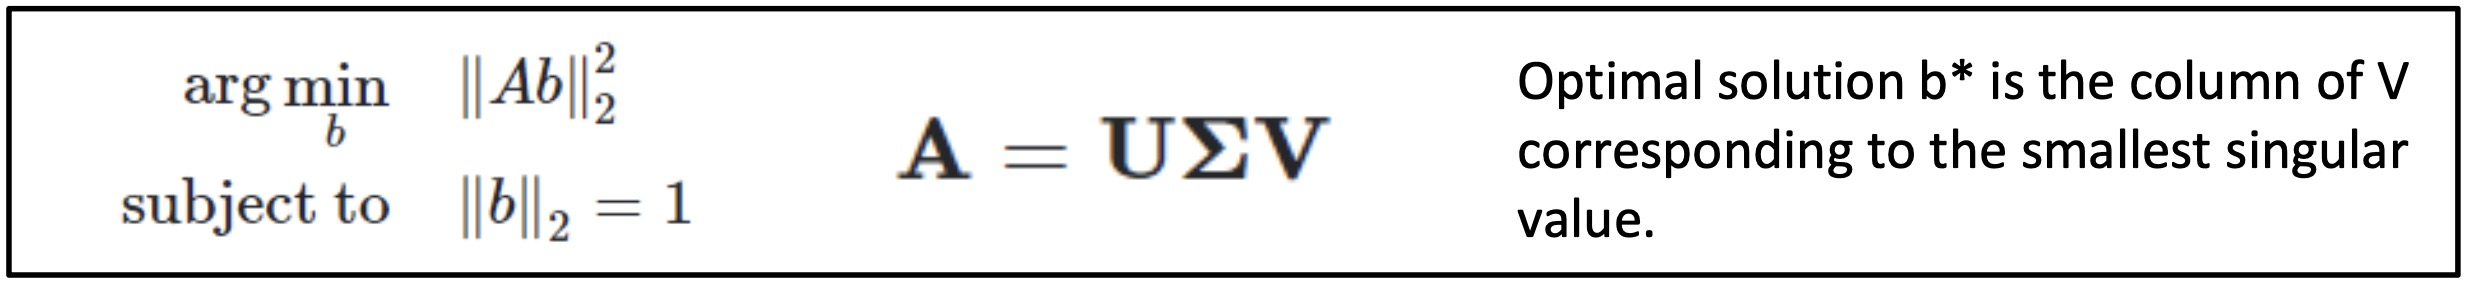
\includegraphics[width=\linewidth]{CV2-Latex-summary/Images/TsaisMethodSVD.jpg}
\end{myfigure}

We recover an orthogonal matrix $\mathbf{R}$, vector $\mathbf{t}$ and an upper-triangular matrix $\mathbf{K}$ from $\mathbf{M}$ using the RQ-decomposition $\mathbf{M}=\mathbf{K}[\mathbf{R}\vert\mathbf{t}]$.
 
\begin{multicols}{2}
    \textbf{In practice}, we use a \textit{single image} with \textit{more than 6 non-coplanar points} (on at least two 3D surfaces). Checkerboard corners can be detected with below 0.1 pixels accuracy.
    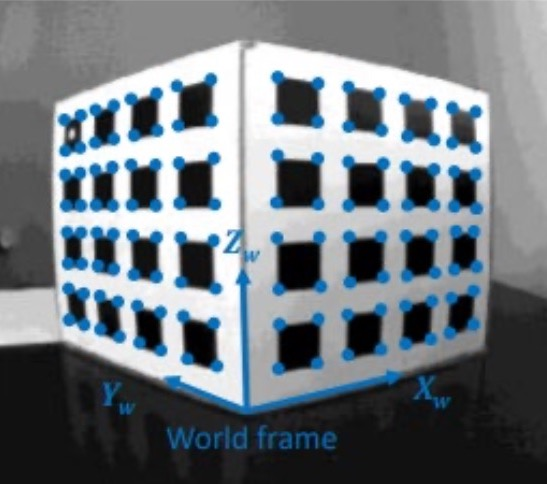
\includegraphics[width=\linewidth]{CV2-Latex-summary/Images/TsaisMethod.jpg}
\end{multicols}

\subsection{Zhang's Method}

\begin{multicols}{2}
    This method works with \textit{3D coplanar points} (allowing to use a planar ``calibration grid''), but relies on multiple images from different views. As opposed to Tsai's method with world coordinate frame is placed in the calibration surface, such that all $Z_w$ values are zero.
    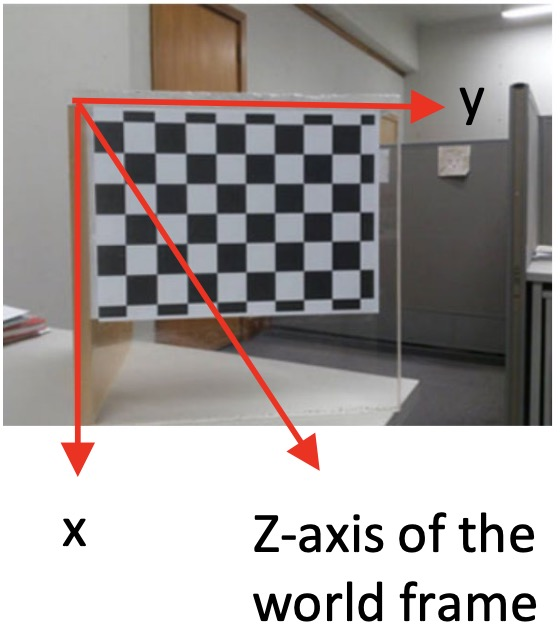
\includegraphics[width=\linewidth]{CV2-Latex-summary/Images/ZhangsMethod.jpg}
\end{multicols} 

\begin{flalign*}
    \lambda\begin{psmallmatrix}u \\v \\1\end{psmallmatrix}
    = \mathbf{K}[\mathbf{R} \mid \mathbf{t}] \begin{psmallmatrix}X_w \\Y_w \\0 \\1\end{psmallmatrix} 
    = \underbrace{\begin{psmallmatrix}
    \alpha_u & 0 & u_0 \\
    0 & \alpha_v & v_0 \\
    0 & 0 & 1
    \end{psmallmatrix} 
    \begin{psmallmatrix}
    r_{11} & r_{12} & t_1 \\
    r_{21} & r_{22} & t_2 \\
    r_{31} & r_{32} & t_3
    \end{psmallmatrix}}_{
    \text{Homography }\mathbf{H}\;\in\;\mathbb{R}^{3\times3}
    } 
    \begin{psmallmatrix}X_w \\Y_w \\1\end{psmallmatrix}
\end{flalign*}

Starting from this equation, we create a system of linear equations with the values of $\mathbf{H}$ as the coefficients in the same fashion as for Tsai's method. 

\begin{flalign*}
    \begin{aligned}
    & u=\frac{\lambda u}{\lambda}=\frac{\mathbf{h}_1^{\mathrm{T}} \cdot \mathbf{p}}{\mathbf{h}_3^{\mathrm{T}} \cdot \mathbf{p}} \\
    & v=\frac{\lambda v}{\lambda}=\frac{\mathbf{h}_2^{\mathrm{T}} \cdot \mathbf{p}}{\mathbf{h}_3^{\mathrm{T}} \cdot \mathbf{p}}
    \end{aligned} 
    \quad\Rightarrow \underbrace{\substack{
    \left(\mathbf{h}_1^{\mathrm{T}}-u \mathbf{h}_3^{\mathrm{T}}\right) \cdot \mathbf{p}=0 \\
    \left(\mathbf{h}_2^{\mathrm{T}}-v \mathbf{h}_3^{\mathrm{T}}\right) \cdot \mathbf{p}=0}
    }_{=\begin{psmallmatrix}
    \mathbf{p}^{\mathrm{T}} & \mathbf{0}^{\mathrm{T}} & -u \mathbf{p}^{\mathrm{T}} \\
    \mathbf{0}^{\mathrm{T}} & \mathbf{p}^{\mathrm{T}} & -v \mathbf{p}^{\mathrm{T}}
    \end{psmallmatrix}
    \begin{psmallmatrix}\mathbf{h}_1 \\\mathbf{h}_2 \\\mathbf{h}_3
    \end{psmallmatrix}=\mathbf{0}}
\end{flalign*} 

Given $n$ 2D-3D point correspondences, the result is $\mathbf{Qh}=\mathbf{0}$, with $\mathbf{Q}\in\mathbb{R}^{2n\times9}$ and the solution vector $\mathbf{h}\in\mathbb{R}^{9}$. For a unique, up-to-scale, non-trivial solution, we require $rank(\mathbf{Q})=8$, such that we need at least 4 non-collinear points.

\paragraph{Recovering $(\mathbf{K, R, t})$ from Multiple Views} Compared to Tsai's method, we cannot obtain $(\mathbf{K, R, t})$ through QR-decomposition, because our modified transformation matrix is not orthogonal. Instead, we use the fact that the intrinsic matrix is constant for all views captured with the same camera. For the $j$th view, we have:

\begin{flalign*}
    \mathbf{H}^j
    = \underbrace{\begin{psmallmatrix}
    h_{11}^j & h_{12}^j & h_{13}^j \\
    h_{21}^j & h_{22}^j & h_{23}^j \\
    h_{31}^j & h_{33}^j & h_{33}^j
    \end{psmallmatrix}}_{[\mathbf{h}_{j1}\;\mathbf{h}_{j2}\;\mathbf{h}_{j3}]}
    = s \cdot \underbrace{\begin{psmallmatrix}
    \alpha_u & 0 & u_0 \\
    0 & \alpha_v & v_0 \\
    0 & 0 & 1
    \end{psmallmatrix}}_{\mathbf{K}}
    \cdot \underbrace{\begin{psmallmatrix}
    r_{11}^j & r_{12}^j & t_1^j \\
    r_{21}^j & r_{22}^j & t_2^j \\
    r_{31}^j & r_{32}^j & t_3^j
    \end{psmallmatrix}}_{[\mathbf{r}_{j1}\;\mathbf{r}_{j2}\;\mathbf{t}_j]}
\end{flalign*}

First, we express the columns of the unkown transformation matrix using the known homographies:

\begin{flalign*}
    \mathbf{r}_{j1}=\lambda\mathbf{K}^{-1}\mathbf{h}_{j1}& \quad\quad
    \mathbf{r}_{j2}=\lambda\mathbf{K}^{-1}\mathbf{h}_{j2} \\
    \mathbf{t}_j=\lambda\mathbf{K}^{-1}\mathbf{h}_{j3}& \quad\quad
    \lambda = s^{-1}
\end{flalign*}

Next, we enforce constraints on our expressions for the rotation (orthogonality and normality):
\begin{flalign*}
    \mathbf{r}^T_{j1}\mathbf{r}_{j2}=0 \quad&\Rightarrow\quad \mathbf{h}^T_{j1}{\color{red}(\mathbf{K}^{-1})^T\mathbf{K}^{-1}}\mathbf{h}_{j2}=0
    \\
    \mathbf{r}^T_{j1}\mathbf{r}_{j1}=\mathbf{r}^T_{j2}\mathbf{r}_{j2}=1 \quad&\Rightarrow\quad \begin{aligned}
        1 &= \mathbf{h}^T_{j1}{\color{red}(\mathbf{K}^{-1})^T\mathbf{K}^{-1}}\mathbf{h}_{j1}\\
        &= \mathbf{h}^T_{j2}{\color{red}\underbrace{(\mathbf{K}^{-1})^T\mathbf{K}^{-1}}_{=\mathbf{B}}}\mathbf{h}_{j2} 
    \end{aligned}
\end{flalign*}
where $\mathbf{B}$ is a $3\times3$ symmetric matrix from which we can \textbf{extract the 6 intrinsic parameters}. We find the solution by solving $\mathbf{A}\mathbf{b}=\mathbf{0}$ where $\mathbf{b}\in\mathbb{R}^6$ is a vector with the relevant values in $\mathbf{B}$ and $\mathbf{A}\in\mathbb{R}^{2n\times6}$ is a matrix with 2 rows (one per constraint) for $n$ views. Mathematically, 3 views are sufficient to find a solution, but we need $n>3$ views in practice. Use the following fact to translate each constraint into a row of $\mathbf{A}$:

\begin{flalign*}
    \mathbf{h}_a^T \mathbf{B} \mathbf{h}_b = \begin{psmallmatrix}
    h_{\mathrm{a}} h_{b 1} \\
    h_{a 1} h_{b 2}+h_{a 2} h_{b 1} \\
    h_{a 2} h_{b 2} \\
    h_{a 3} h_{b 1}+h_{a 1} h_{b 3} \\
    h_{a 3} h_{b 2}+h_{a 2} h_{b 3} \\
    h_{a 3} h_{b 3}
    \end{psmallmatrix}^T\begin{psmallmatrix}B_{11} \\B_{12} \\B_{22} \\B_{13} \\B_{23} \\B_{33}
    \end{psmallmatrix}
\end{flalign*}

Next, we \textbf{extract the extrinsic parameters} for each view. E.g. for the $j$th view, the transformation matrix becomes:

\begin{flalign*}
    [\mathbf{R}|\mathbf{t}]^j=
    \begin{psmallmatrix}
    \vert&\vert&\vert&\vert\\
    \mathbf{r}_{j1}&\mathbf{r}_{j2}&(\mathbf{r}_{j1}\times\mathbf{r}_{j2})&\mathbf{t}_j\\
    \vert&\vert&\vert&\vert\\
    \end{psmallmatrix}
\end{flalign*}

\subsection{Image Undistortion}
We account for distortion, by modifying the perspective projection model from camera to pixel coordinates by including \textbf{tangential and radial distortion coefficients}, denoted $k_n$ and $p_n$ respectively. Instead of $u=f_x y+c_x$ and $v=f_y y+c_y$ with image coordinates $(x\;y\;1)^T$, we have:

\begin{flalign*}
    u=f_x x_\text{dist}+c_x \quad\text{and}\quad v=f_y y_\text{dist}+c_y
\end{flalign*}

using some polynomal distortion model, e.g.:

\begin{flalign*}
    &x_\text{dist}=x \frac{1+k_1 r^2+k_2 r^4+k_3 r^6}{1+k_4 r^2+k_5 r^4+k_6 r^6}+2 p_1 x y+p_2 
    \\
    &y_\text{dist}=y \frac{1+k_1 r^2+k_2 r^4+k_3 r^6}{1+k_4 r^2+k_5 r^4+k_6 r^6}+p_1\left(r^2+2 y^2\right)+2 p_2 x y
    \\
    &\text{with }r^2=x^2+y^2
\end{flalign*}

Then, we find the distortion coefficients by:
\begin{enumerate}
    \item Initially setting $p_n=k_n=0$.
    \item Performing Zhang's method to obtain a good ``initial guess'' of the intrinsic and extrinsic parameters.
    \item Projecting the world-space points using the computed projection matrix and calculating the re-projection error between the computed and detected image-space points.
    \item Minimizing the error with gradient descent jointly w.r.t.\ the intrinsic, extrinsic and distortion parameters: $$\underset{\mathbf{K},\mathbf{R},\mathbf{t},k_1,p_1,...}{\text{argmin}}\sum^n_{i=1}\norm{\mathbf{p}^i-\pi(\mathbf{P}^i_W,\mathbf{K},\mathbf{R},\mathbf{t},k_1,p_1,...)}^2$$
\end{enumerate}

\begin{myfigure}
    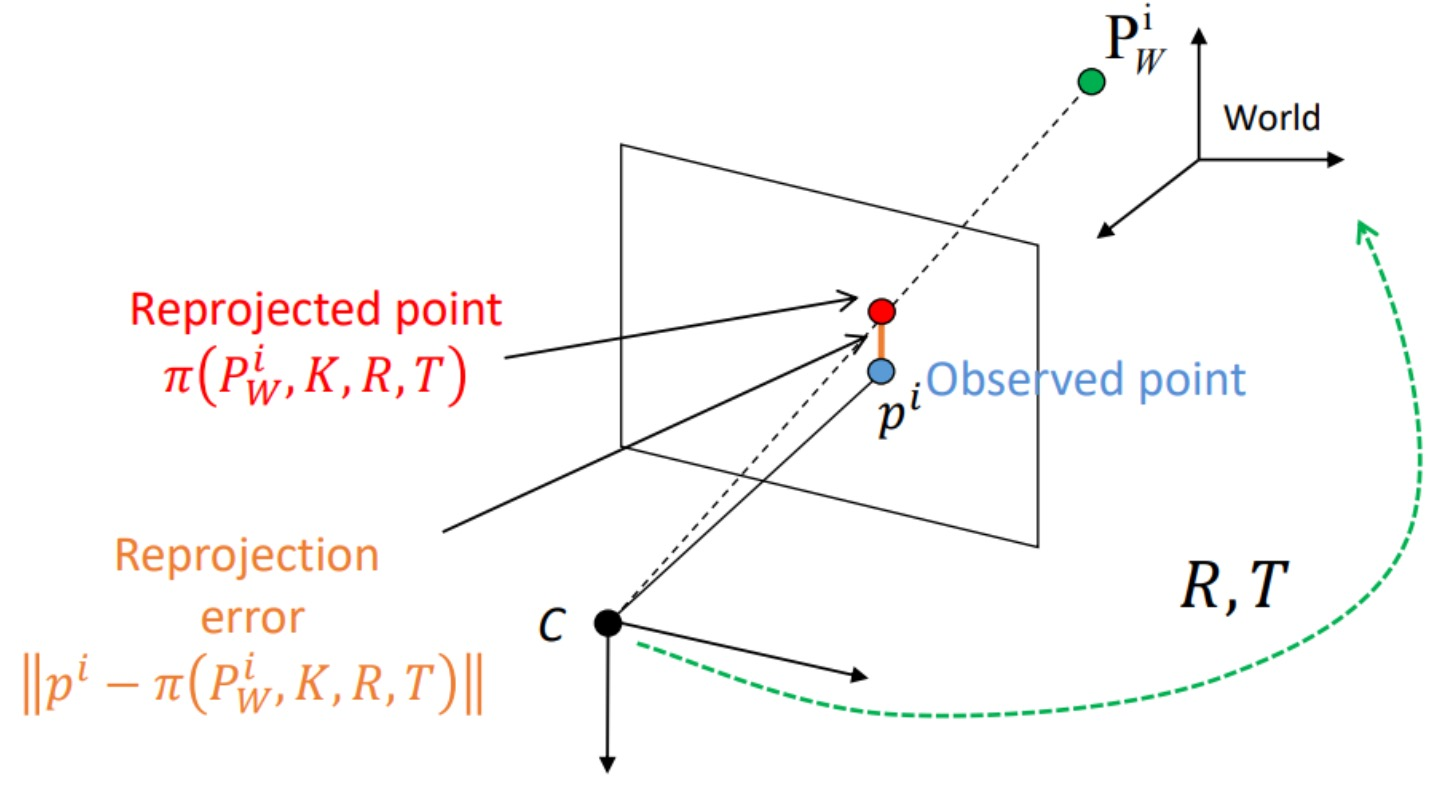
\includegraphics[width=\linewidth]{CV2-Latex-summary/Images/DistortionError.jpg}
\end{myfigure}

\paragraph{Line-based Undistortion} Another approach to image undistortion is by finding the intrinsic, extrinsic and distortion parameters that lead to vanishing points which maximize the number of inlier lines.

\begin{myfigure}
    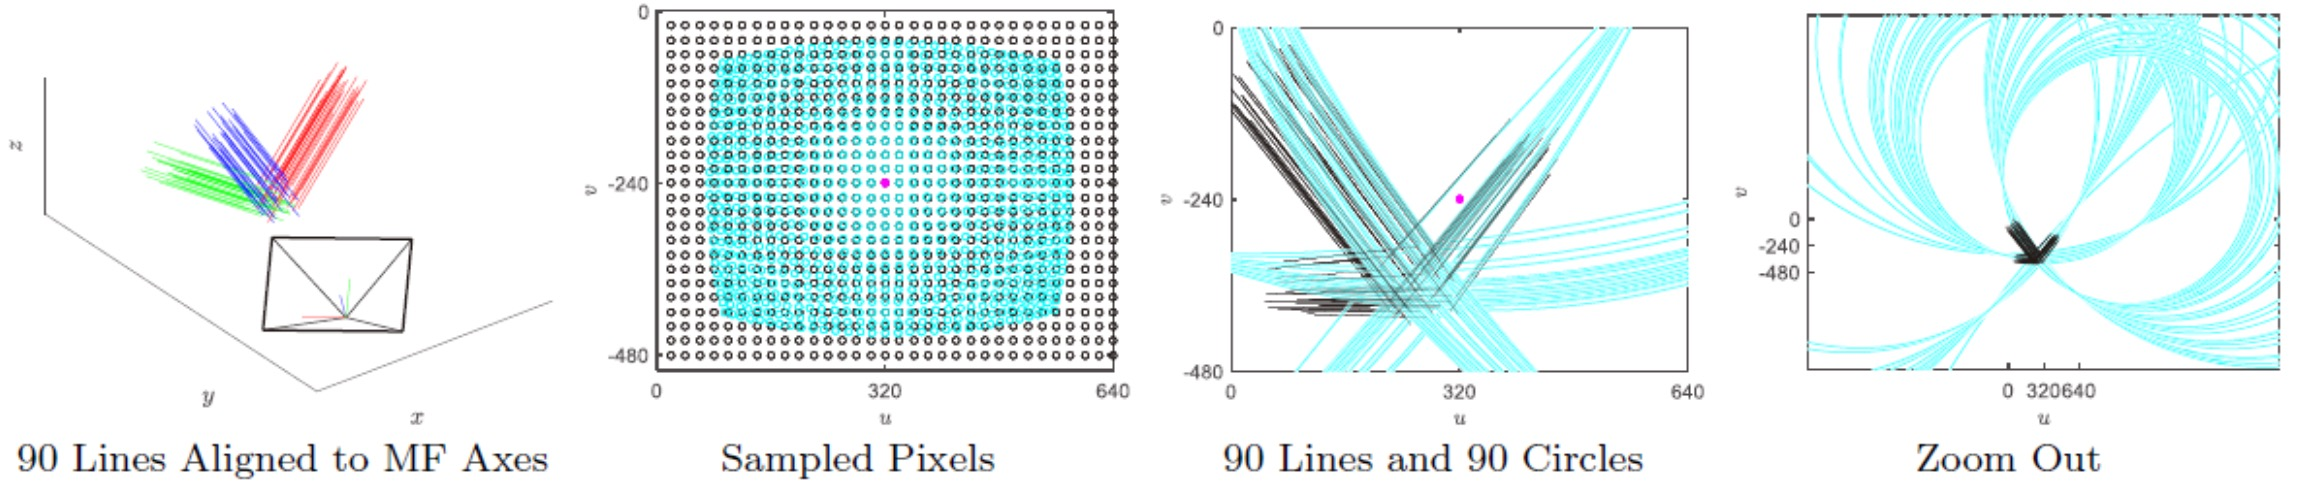
\includegraphics[width=\linewidth]{CV2-Latex-summary/Images/LineBasedUndistortion.jpg}
\end{myfigure}

\end{multicols}
\newpage

% #############################
% ### POINT CORRESPONDENCES ###
% #############################

\begin{multicols}{2}[\section{Estimating Point Correspondences}]

In practice, we observe characteristic image features like brightness or color values at individual pixels instead of points or lines. There exist two types of point matching strategies: direct and indirect methods. \textbf{Direct methods} exploit all information in an image, leading to higher accuracy and robustness, have reduced computational cost with higher frame rates (since no RANSAC is needed), but are sensitive to initialisation and only work with small frame-to-frame motions. \textbf{Indirect methods} work by detecting and matching features (points/lines), can cope with large frame-to-frame motions and strong illumination changes, but are slow due to costly feature extraction, matching and outlier removal.

\subsection{Direct Methods (Optical Flow; Small Motion)}
Direct methods make use of the apparent 2D motion field observable between consecutive images of a video, known as \textbf{optical flow}, which differs from the motion of objects in the scene. They estimate the parameters $\mathbf{p}$ of a transformation $W(\mathbf{x},\mathbf{p})$ from a template image $T$ to a new image $I$, by processing the change in pixel intensities. Every yellow dot in the image below represents a tracked pixel.

\begin{center}
    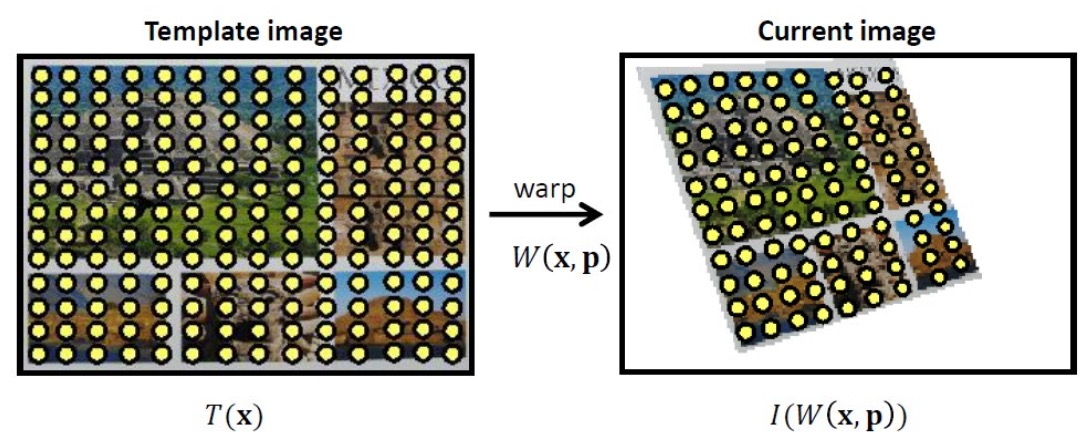
\includegraphics[width=0.8\linewidth]{CV2-Latex-summary/Images/OpticalFlowWarp.jpg}
\end{center}

Note that this is a \textit{chicken-and-egg problem}, because we have two unknown parameters (the corresponding pixels and the transformation parameters) that are mutually determined. In practice, we solve the problem by adding constraints, such as constant brightness for corresponding pixels.

\paragraph{We make the following assumptions:} Let $\mathbf{x}(t)$ denote a moving point at time $t$, and $I(\mathbf{x},t)$ a pixel intensity in a video sequence.
\begin{enumerate}
	\item \textbf{Brightness constancy (``optical flow constraint'')}: the brightness of the pixels to track does not change over consecutive frames, i.e.\ $I(\mathbf{x}(t),t) = \text{const.}, \, \forall t $. It follows that
    $$\frac{d}{dt}I(\mathbf{x}(t),t) = \nabla I^T \frac{d\mathbf{x}}{dt} + \frac{\partial I}{\partial t} = 0$$.
	\item \textbf{Temporal consistency}: the motion $\mathbf{v}$ is constant over a neighborhood $\Omega$ around  $\mathbf{x}$:
    $$\nabla I(\mathbf{x}',t)^T \mathbf{v} + \frac{\partial I}{\partial t}(\mathbf{x}',t) = 0, \,\quad \forall x' \in \Omega$$
    The frame-to-frame motion should measure only 1-2 pixels in practice.
    \item \textbf{Spatial coherence}: All pixels in the template undergo the same transformation, which requires all points to lie on the same 3D surface and unusual in practice.
\end{enumerate}

\subsubsection{Kanade-Lucas-Tomasi (KLT) Tracker}

This method solves two sub-problems: the \textbf{Tomasi-Kanade method} selects the most reliable image features/patches for tracking and the \textbf{Lucas-Kanade method} tracks/aligns these image features/patches.

\begin{wrapfigure}{r}{0.4\linewidth}
    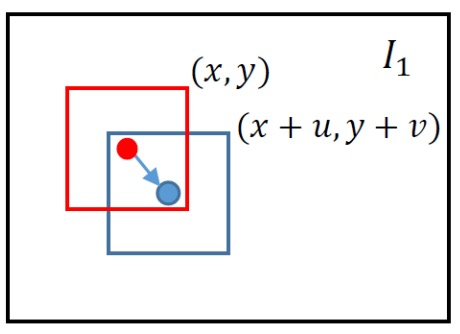
\includegraphics[width=\linewidth]{CV2-Latex-summary/Images/OpticalFlowTranslation.jpg}
\end{wrapfigure}
\paragraph{Simplified Case (Pure Translation)} We assume that all pixels in the template are moved by the same motion vector $(u\;v)^T$ between the template image $I_0$ and a new image $I_1$ (which is usually never the case). Now, we want to minimize the sum of squared differences (SSD) between intensities of corresponding pixels in the template and the new image:

\begin{flalign*}
    \text{SSD}(u,v)&=\sum_{x,y\in\Omega}(I_0(x,y)-\underbrace{I_1(x+u,y+v)}_{\approx I_1(x,y)+\frac{\partial I_1}{\partial x}u+\frac{\partial I_1}{\partial y}v})^2
    \\
    &\approx \sum_{x,y\in\Omega}(\Delta I-I_x u-I_y v)^2
\end{flalign*}

where $\Omega$ is the size of the image patch that we select for tracking, $\Delta I$ is the intensity change at $(x,y)$ and $\nabla I=(I_x\;I_y)^T$ are the partial derivatives of $I_1$ at $(x,y)$. We obtain a solution from the first-order optimality condition:

\begin{flalign*}
    &\nabla\text{SSD}\approx\begin{psmallmatrix}
        -2\sum I_x(\Delta I-I_x u-I_y v)\\
        -2\sum I_y(\Delta I-I_x u-I_y v)
    \end{psmallmatrix}
    = \mathbf{0}
    \\
    &\Rightarrow
    \underbrace{\begin{psmallmatrix}
        \sum I^2_x & \sum I_x I_y\\
        \sum I_x I_y & \sum I^2_y
    \end{psmallmatrix}}_{\mathbf{M}}
    \begin{psmallmatrix}u \\ v\end{psmallmatrix}
    = \underbrace{\begin{psmallmatrix}\sum I_x \Delta I\\\sum I_y \Delta I\end{psmallmatrix}}_{=\mathbf{b}}
\end{flalign*}

If $\mathbf{M}$ is invertible, we obtain the motion vector $(u\;v)^T=\mathbf{M}^{-1}\mathbf{b}$. Therefore, we need to ensure that $\det(\mathbf{M})=\lambda_1\lambda_2\cdots\lambda_n\neq0$, by \textbf{selecting an image patch, whose coefficient matrix $\mathbf{M}$ has large eigenvalues}. 
\begin{wrapfigure}{r}{0.4\linewidth}
    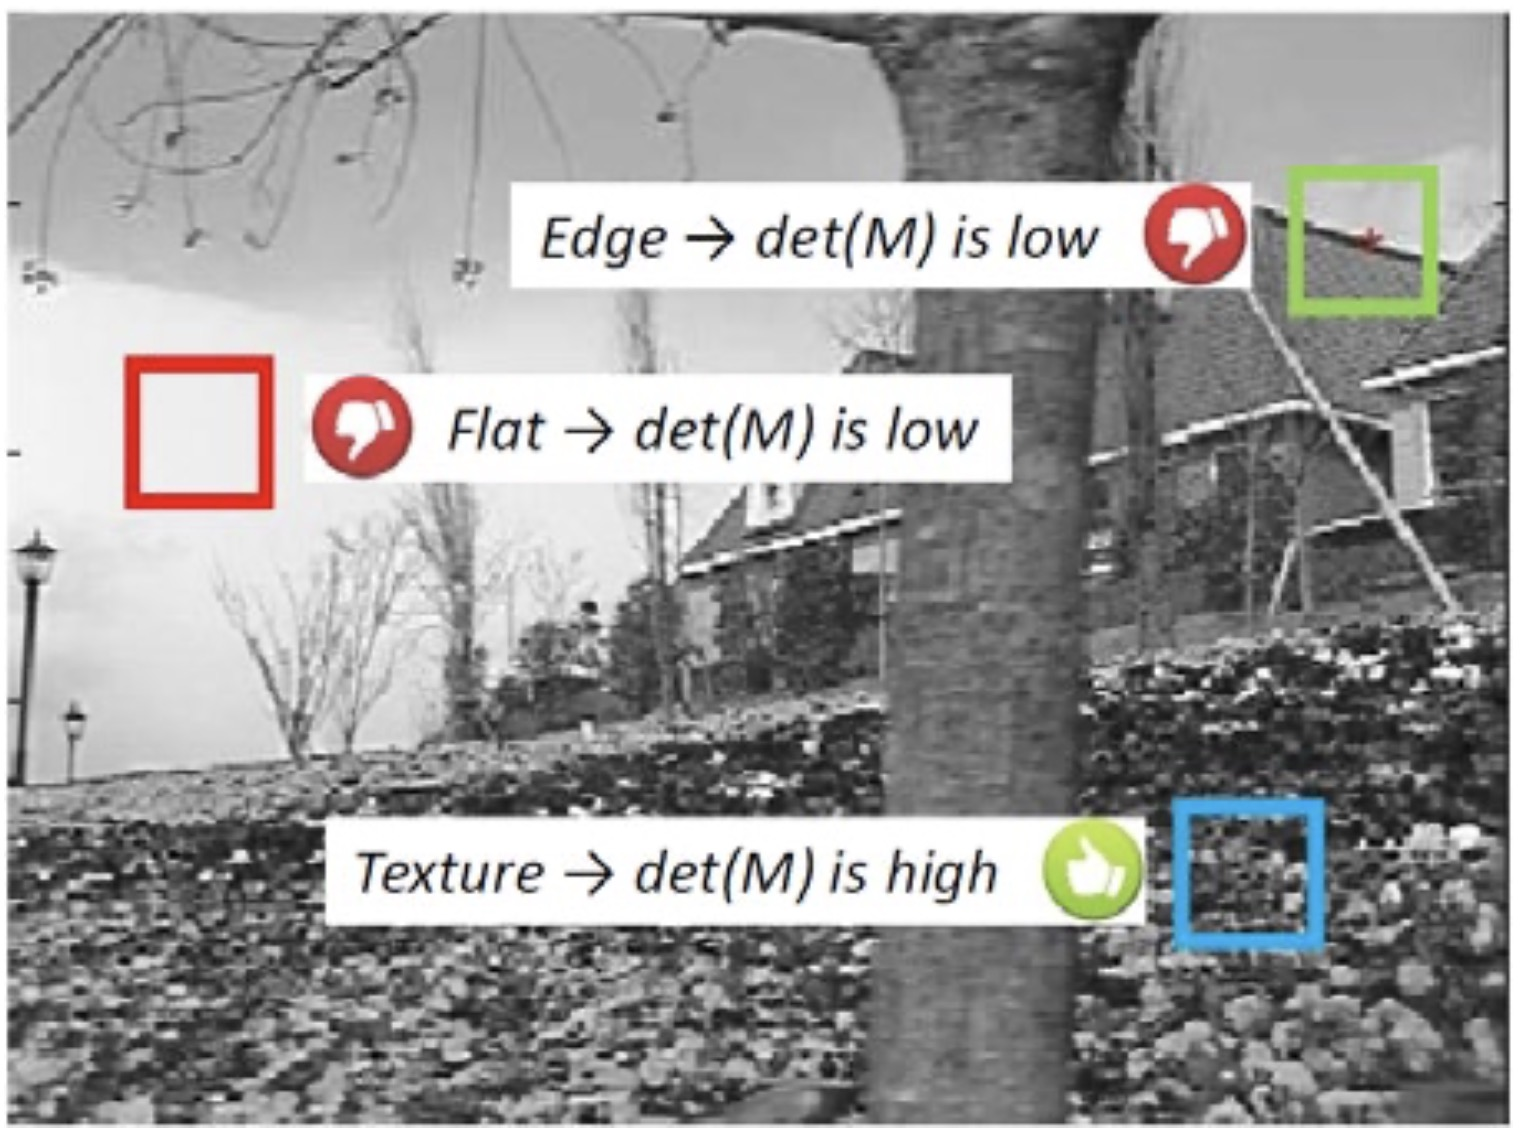
\includegraphics[width=\linewidth]{CV2-Latex-summary/Images/MMatrixDeterminant.jpg}
\end{wrapfigure}
Edges and flat patches for instance results in low and textured patches result in high determinants. Then, we \textbf{track the image patch along the computed motion vector}. In practice, we select good patches in the first image and track the same points in all subsequent images.

\paragraph{General Case (Warping)} We assume that all pixels in the template image $T$ undergo a warping transformation with the parameters $\mathbf{p}$:

\begin{flalign*}
    \text{SSD} = \sum_{\mathbf{x}\in T}[\underbrace{I(W(\mathbf{x},\mathbf{p}+\Delta\mathbf{p}))}_{\approx I(W(\mathbf{x},\mathbf{p}))+\nabla I\frac{\partial W}{\partial \mathbf{p}}\Delta\mathbf{p}}-T(\mathbf{x})]^2
\end{flalign*}

where we simplify the warping transformation using the first-order Taylor approximation. Finding the parameters $\mathbf{p}$ that minimize this constraint with the first-order optimality condition is difficult. Instead, we leverage the Gauss-Newton method to minimize the SSD iteratively. We obtain the parameter update vector by equating $\frac{\partial\text{SSD}}{\partial\Delta\mathbf{p}}$ to zero and solving for $\Delta \mathbf{p}$:

{\small
\begin{flalign*}
    &2\sum_{\mathbf{x}\in T} \left[\nabla I\frac{\partial W}{\partial \mathbf{p}}\right]^T \left[I(W(\mathbf{x},\mathbf{p}))+\nabla I\frac{\partial W}{\partial \mathbf{p}}\Delta\mathbf{p}-T(\mathbf{x})\right] = 0
    \\
    &\Rightarrow \Delta\mathbf{p} = H^{-1} \sum_{\mathbf{x}\in T} \left[\nabla I\frac{\partial W}{\partial \mathbf{p}}\right]^T [T(\mathbf{x})-I(W(\mathbf{x},\mathbf{p}))]
    \\
    &\text{with }H = \sum_{\mathbf{x}\in T} \left[\nabla I\frac{\partial W}{\partial \mathbf{p}}\right]^T \left[\nabla I\frac{\partial W}{\partial \mathbf{p}}\right]
\end{flalign*}
}
\paragraph{Alternative Derivation of the General Case} The Lucas-Kanade method generates sparse flow vectors under the assumption of constant motion in a local neighborhood (temporal consistency assumption). It follows that the least square error of point $\mathbf{x}$ is:
\begin{flalign*}
    E(\mathbf{v}) &= \int_{W(\mathbf{x})} | \nabla I(\mathbf{x}',t)^T \mathbf{v} + I_t (\mathbf{x}',t)|^2 d\mathbf{x}' \\
    &= \mathbf{v}^T \mathbf{M} \mathbf{v} + 2 \mathbf{q}^T \mathbf{v}
\end{flalign*}
\begin{flalign*}
    \text{with }\mathbf{M} = \int_{W(x)} \nabla I \nabla I^T \;\mathrm{d}\mathbf{x'}& 
    \quad\quad 
    \mathbf{q} = \int_{W(x)} I_t \nabla I \;\mathrm{d}\mathbf{x'} 
    \\
    \nabla I = \begin{pmatrix}I_x \\I_y \end{pmatrix} = \begin{pmatrix}\frac{\partial I}{\partial x} \\ \frac{\partial I}{\partial y} \end{pmatrix}& 
    \quad\quad
    I_t = \frac{\mathrm{d}I}{\mathrm{d}t}
\end{flalign*}
We set $\frac{dE}{d\mathbf{v}} = 0$ to get the local flow vector (velocity):
\begin{equation*}
	\mathbf{v} = \frac{d\mathbf{x}}{dt} = -\mathbf{M}^{-1}\mathbf{q}
\end{equation*}
given that $\mathbf{M}$ is invertible ($\det(\mathbf{M}) \neq 0$). $\mathbf{M}$ is PSD.

\begin{equation*}
    \text{Solution: }\quad \mathbf{v} = \begin{pmatrix} \frac{m_{22} q_1 - m_{12} q_2}{m_{12}^2 - m_{11} m_{22}} \\ \frac{m_{11} q_2 - m_{12} q_1}{m_{12}^2 - m_{11} m_{22}} \end{pmatrix}
    \in \mathbb{R}^2
\end{equation*}
\paragraph{Aperture problem} It is impossible to determine the motion $\mathbf{v}$ orthogonal to the gradient direction $\nabla \mathbf{I}$ in regions with constant gradient direction. In these regions $\det\mathbf{M}=0$.

\paragraph{KLT Tracker Algorithm}

\begin{enumerate}
    \item For time $t$, at each point $\mathbf{x} \in \Omega$ compute:
    \begin{equation*}
    M(x) = \int_{\Omega} \begin{pmatrix}I_x^2 & I_xI_y\\I_xI_y & I_y^2 \end{pmatrix} \;\mathrm{d}\mathbf{x}'.
    \end{equation*}
    \item Keep all points $\mathbf{x} \in \Omega$ for which $\det(\mathbf{M}(\mathbf{x}))$ is greater or equal to a threshold $\theta > 0$.
    \item The local velocity of these points is given by:
    \begin{equation*}
        \mathbf{b}(\mathbf{x}, t) = -\mathbf{M}(\mathbf{x})^{-1} \begin{pmatrix}\int I_xI_t \;\mathrm{d}\mathbf{x}'\\ \int I_yI_t \;\mathrm{d}\mathbf{x}' \end{pmatrix}.
    \end{equation*}
    \item Repeat for the points $\mathbf{x}+\mathbf{b}$ at time $t+1$.
\end{enumerate}

\subsection{Indirect Methods (Large Motion)} 

We compute the transformation between two images by: \textbf{1) detecting and matching features}; \textbf{2) computing the transformation} and 3) optionally refining the initial estimate by minimizing a squared sum of reprojection errors.

\begin{myfigure}
    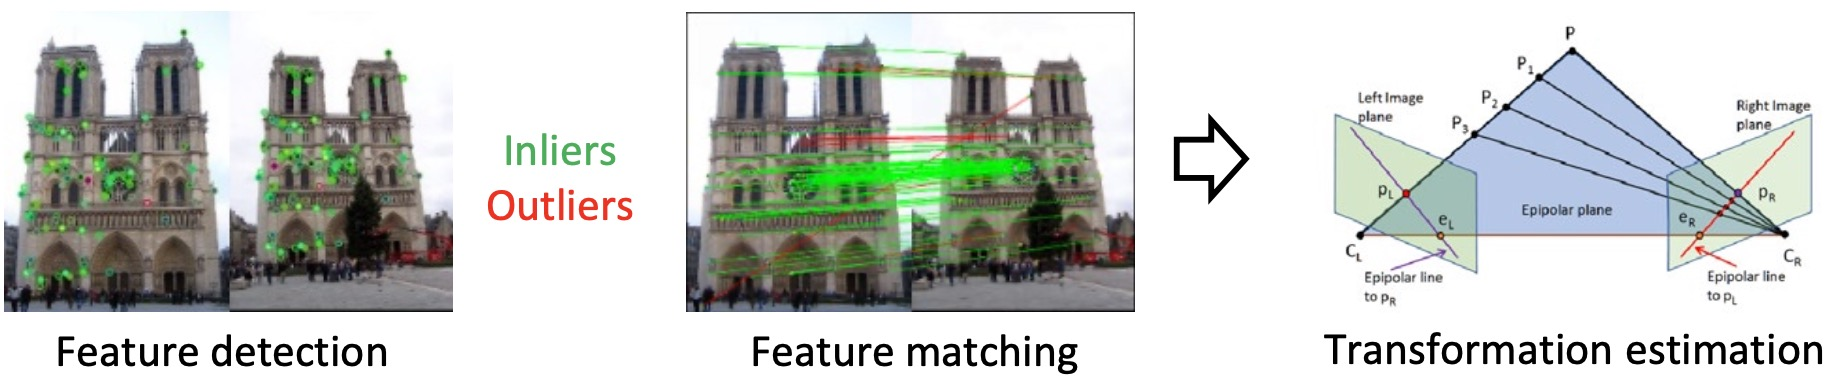
\includegraphics[width=\linewidth]{CV2-Latex-summary/Images/IndirectMethodStrategy.jpg}
\end{myfigure}

\subsubsection{Feature Detectors} 

The feature detector is responsible for detecting and matching features that are invariant to scale, rotation and view point changes. A \textbf{blob} is a group of connected pixels in an image that share some common property (e.g.\ the same grayscale value). Blobs have less localization accuracy than corners, but are more distinctive. A \textbf{corner} is defined a the intersection of two or more edges. They have high localization accuracy, but are less distinctive than blobs.

\paragraph{Moravec's Corner Detector} In the region around a corner, the image gradient is large in all directions, which is not true for edges or flat regions. Thus, shifting a window horizontally, vertically or diagonally should cause large intensity changes around a corner. For a given patch:
\begin{enumerate}
    \item compute the SSD between all pairs of corresponding pixels when shifting the window along all directions, e.g. for a shift $\Delta \mathbf{x}$:
    {\small
    $$\text{SSD}(\Delta\mathbf{x})=\sum_{\mathbf{x}\in\Omega}(I(\mathbf{x})-I(\mathbf{x}+\Delta \mathbf{x})^2$$
    }
    \item keep the lowest SSD (\textit{interest measurement}),
    \item if the interest measurement is higher than a threshold, the patch center is a corner.
\end{enumerate}

\paragraph{Harris' Corner Detector} This is an \textbf{efficient} version of Moravec's method, since it does not explicitly shift the window. We approximate the SSD:
\begin{flalign*}
    \text{SSD}(\Delta \mathbf{x})&\approx\sum_{\mathbf{x}\in\Omega}(I_x(\mathbf{x})\Delta x+I_y(\mathbf{x})\Delta y)^2
    \\
    &\approx 
    \underbrace{\begin{psmallmatrix}\Delta x&\Delta y\end{psmallmatrix}}_{\substack{\text{manually}\\\text{assigned}}}
    \underbrace{\begin{psmallmatrix}
        \sum I_x^2 & \sum I_x I_y\\
        \sum I_x I_y & \sum I_y^2
    \end{psmallmatrix}}_{\substack{\mathbf{M},\text{ encodes the}\\\text{SSD change}}} 
    \begin{psmallmatrix}\Delta x\\\Delta y\end{psmallmatrix}
\end{flalign*}
\begin{wrapfigure}{r}{0.4\linewidth}
    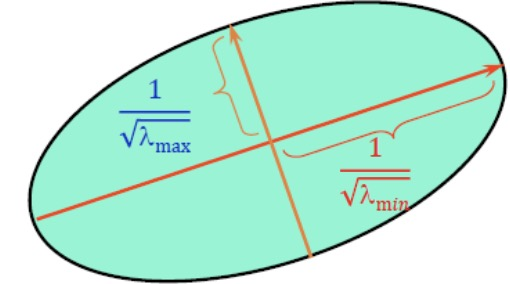
\includegraphics[width=\linewidth]{CV2-Latex-summary/Images/HarrisCornerDetectorM.jpg}
\end{wrapfigure}
We can efficiently compute $\mathbf{M}$ using  $\mathbf{M}=\mathbf{R}^{-1}\mathbf{\Lambda}\mathbf{R}$, using the eigenvector matrix $\mathbf{R}$ and diagonal eigenvalue matrix $\mathbf{\Lambda}$, where the largest eigenvalue corresponds to the direction of the quickest intensity change. Accordingly, both eigenvalues should be large for a corner-patch.
\begin{myfigure}
    \centering
    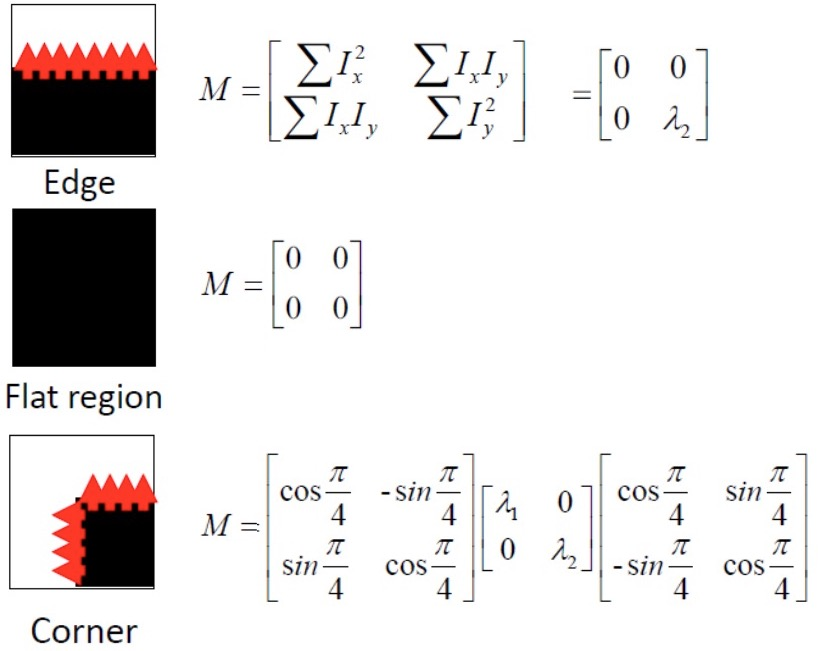
\includegraphics[width=0.7\linewidth]{CV2-Latex-summary/Images/EigenvaluesCorner.jpg}
\end{myfigure}
Harris' corner detector is \textbf{not scale invariant}, because the window size is fixed. 

\subsubsection{Feature Matching}

\paragraph{Feature Descriptor} Each detected feature (pixel/patch/blob) is described by one or more \textit{descriptors}, which describes the pixel information around a feature as a scalar or vector. It should be \textit{distinctive} (unique w.r.t.\ other features), \textit{robust to geometric} (scale-, rotation- \& view-point-invariance) and \textit{illumination changes}. 

\paragraph{Brute Force Matching} Given two images with $N$ features each, nearest neighbors search requires $N^2$ comparisons. Validating each right-image-patch  at $S$ tentative scales for all $N$ left-image-patches creates  the complexity $\mathcal{O}(N^2S)$. Another drawback of this method is that we assume the scale of the left images' patches as optimal. We avoid unreliable points at repetitive image patterns, by comparing the ratio of distances to the 1st and 2nd closest descriptors to a threshold. 

\paragraph{General Pipeline} Given two feature descriptors  $H(\mathbf{x})$ and $F(\mathbf{x})$ from different images:
\begin{enumerate}
    \item \textbf{Determine the scale, rotation and viewpoint change of each patch.} We determine the \textit{scale} by assigning a function to each patch, that maps the patch size $\sigma$ to some value and has extrema that are invariant to the path size. Then, the sizes $\sigma_1$ and $\sigma_2$ at which the functions associated to two patches achieve (the same) extremum are the sizes at which the patches have the same scale (correspond to the same 3D area). 
    \begin{center}
        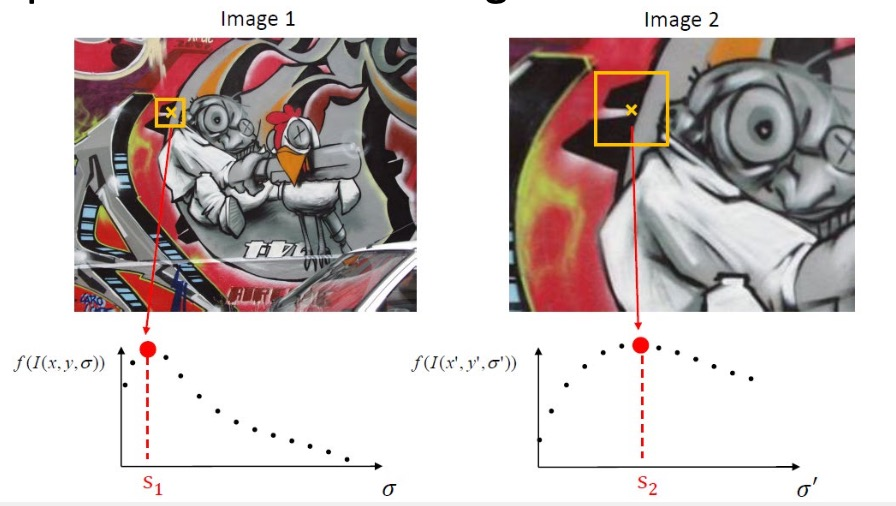
\includegraphics[width=0.8\linewidth]{CV2-Latex-summary/Images/FeatureDescriptorScale.jpg}
    \end{center}
    Our function is a convolution of the image with the Laplacian of the Gaussian kernel (LoG):
    {\small$$
        \text{LoG}(x,y,\sigma) = \nabla^2 G_\sigma(x,y) = \frac{\partial^2 G_\sigma(x,y)}{\partial x^2} + \frac{\partial^2 G_\sigma(x,y)}{\partial y^2}
    $$}
    where $\sigma=\frac{r}{\sqrt{2}}$ is the kernel ``radius'' (scale) and needs adjustment. Mathematically, we find the scale that leads to the maximum convolution response with the image patch (e.g.\ a blob).
    \begin{center}
        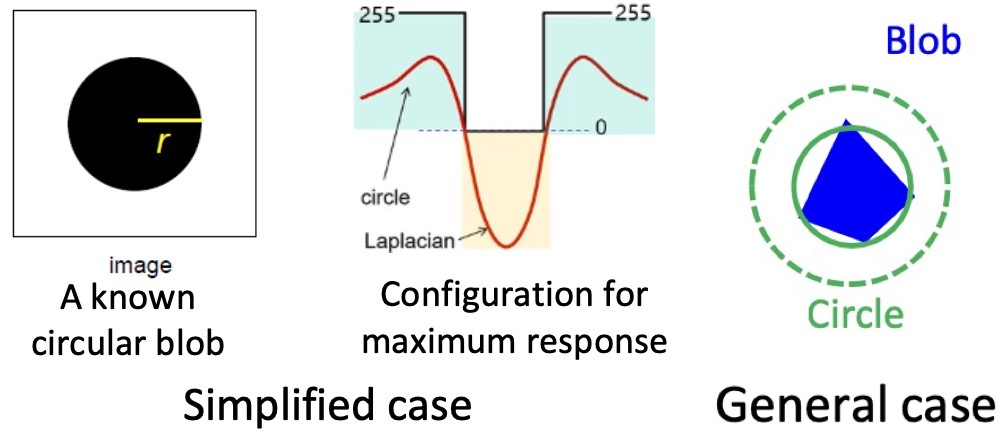
\includegraphics[width=.8\linewidth]{CV2-Latex-summary/Images/LaplacianOfGaussian.jpg}
    \end{center}
    In practice, we find $\sigma$ by trying some candidates. Once $\sigma_1$ and $\sigma_2$ are known, we can rescale both patches to a canonical patch size. This way, we determine the \textbf{scale of each patch individually \& automatically}. We filter overlapping blobs using non-maximum-suppression (NMS). 
    
    Next, we find the patch \textit{rotation} via the eigenvectors of its Harris' matrix $\mathbf{M}$ or by extracting the dominant directions from a histogram of pixel-gradient-directions. 
    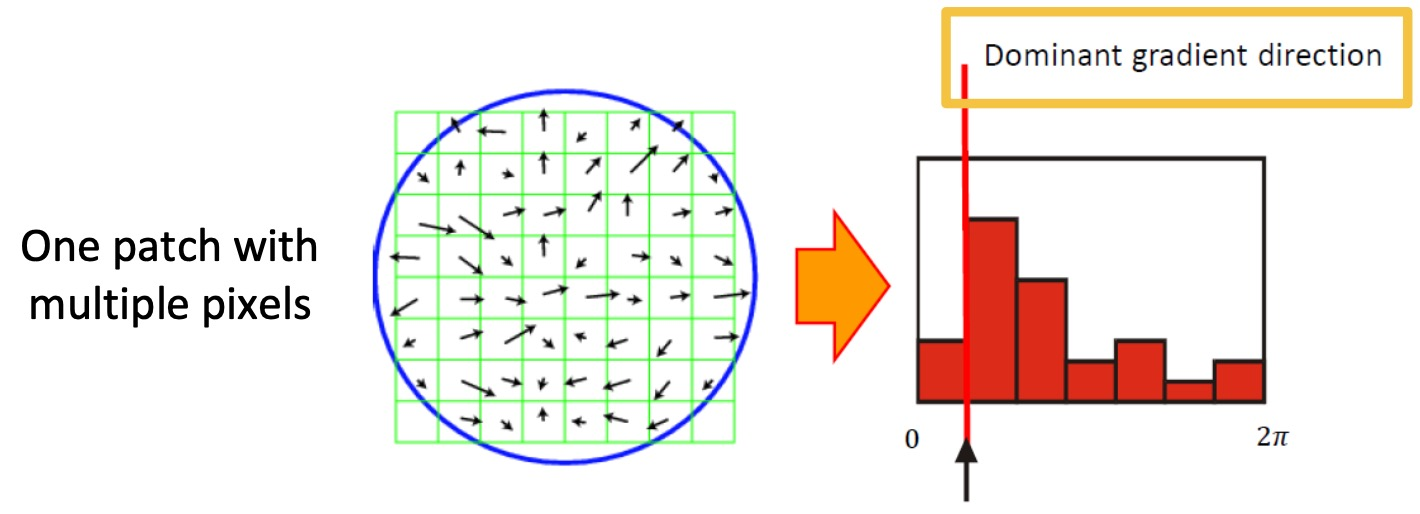
\includegraphics[width=\linewidth]{CV2-Latex-summary/Images/PixelGradientDirections.jpg}

    Finally, we account for the \textit{viewpoint}, by computing the computing the $\mathbf{M}$ matrix and normalizing the ellipse that results from its eigenvectors and eigenvalues into a circular patch.
    
    \item \textbf{Warp each patch into a canonical patch.}
    \begin{center}
        \includegraphics[width=0.8\linewidth]{CV2-Latex-summary/Images/FeatureDetectors.jpg}
    \end{center}
    \item \textbf{Establish patch correspondences based on  similarity of the warped patches} using brute force search and the sum of squared differences (SSD), sum of absolute differences (SAD) or normalized cross correlation (NCC):
    {\footnotesize
    \begin{flalign*}
        &\text{SSD}=\sum_{\mathbf{x}\in\Omega}(H(\mathbf{x})-F(\mathbf{x}))^2 \in [0, \infty)
        \\
        &\text{SAD}=\sum_{\mathbf{x}\in\Omega}\vert H(\mathbf{x})-F(\mathbf{x})\vert \in [0, \infty)
        \\
        &\text{NCC}=\frac{\sum\limits_{\mathbf{x}\in\Omega}(H(\mathbf{x})-\mu_H) (F(\mathbf{x})-\mu_F)}{\sqrt{\sum\limits_{\mathbf{x}\in\Omega}(H(\mathbf{x})-\mu_H)^2} \sqrt{\sum\limits_{\mathbf{x}\in\Omega}(F(\mathbf{x})-\mu_F)^2}} \in [-1, 1]
        \\
        &\text{with }\mu_H=\frac{1}{\vert\Omega\vert}\sum_{\mathbf{x}\in\Omega}H(\mathbf{x}) \quad\quad \mu_F=\frac{1}{\vert\Omega\vert}\sum_{\mathbf{x}\in\Omega}F(\mathbf{x})
    \end{flalign*}}
    where $\mu_H$ and $\mu_F$ are used to account for the difference in average intensity of the two images.
\end{enumerate}

The ``automatic'' matching strategy allows to determine the scale (out of $S$ candidates) for $N$ patches per image before doing the matching (complexity $\mathcal{O}(2NS+N^2)$). The drawback of this pipeline, is that small errors/noise in rotation, scale and variance will affect the warping and thus the matching score.

\subsubsection{Scale-invariant Feature Transform (SIFT)}

Instead of comparing the pixels of warped patches with SSD (patch descriptors), we compare the \textbf{census descriptors} associated with those warped patches, which is less sensitive to noise. We extract key points via the more efficient \textit{difference of Gaussian} (DoG) kernel:
\begin{flalign*}
    \text{LoG}(x,y)\approx\text{DoG}(x,y)=G_{k\sigma}(x,y)-G_{\sigma}(x,y),
\end{flalign*}
\begin{wrapfigure}{r}{0.6\linewidth}
    \includegraphics[width=\linewidth]{CV2-Latex-summary/Images/FirstStepOfSIFT.jpg}
\end{wrapfigure}
where we \textbf{first apply two Gaussian kernels at different scales} $k\sigma$ to an image (producing two blurred images of the same size) and then take their difference. 

We compare each pixel a DoG image to its 26 neighbors (8 at the same scale and 9 at the adjacent lower and upper scales respectively). If the pixel is a local extrema w.r.t.\ its neighbors it is a SIFT feature/keypoint $(x, y, k\sigma)$. 
\begin{wrapfigure}{r}{0.6\linewidth}
    \includegraphics[width=\linewidth]{CV2-Latex-summary/Images/DoG.jpg}
\end{wrapfigure}
Optionally, we obtain additional keypoints by finding local maxima in the DoG images at multiple down-scaled resolution (a.k.a.\ at different \textit{octaves}). We compute the \textit{census descriptor} of a keypoint by considering the circular region around it, where the radius is determined by $\sigma$, and de-rotating the patch according to its dominant direction. \textbf{Secondly}, we divide the patch into e.g.\ $4\times4$ cells, generate histograms with the 8 dominant gradient directions for of each cell and concatenate all histograms into a 1D vector (the SIFT feature).
\begin{center}
    \includegraphics[width=\linewidth]{CV2-Latex-summary/Images/SIFTFeature.jpg}
\end{center}
The complete output of the algorithm is: 
\begin{itemize}
    \item the patch location $(x, y)$,
    \item the patch scale $k\sigma$,
    \item the patch orientation and
    \item the $4\times4\times8=128$ element-long 1D vector.
\end{itemize}
\subsection{Deep Learning-based Method: SuperPoint}

This architecture (``Self Supervised Interest Point Detection and Description'', 2018) regresses the keypoint locations and the descriptor feature vectors simultaneously. Its keypoint detections are less accurate than SIFT and it is less efficient, but its descriptors are better. 
\begin{center}
    \includegraphics[width=\linewidth]{CV2-Latex-summary/Images/SuperPoint.jpg}
\end{center}

\end{multicols}

\newpage
\begin{multicols}{2}[\section{2D-2D Geometry (Reconstruction from Two Views: Linear Algorithms)}]

\subsection{The Reconstruction Problem}
We assume, that (1) a \textbf{set of corresponding points in two frames} from the same camera is given; (2) the \textbf{intrinsic camera parameters are known}; and (3) the \textbf{scene is static}.

We estimate the relative transformation between camera frames and then perform 3D reconstruction by triangulation.

\paragraph{Scale Ambiguity} This is the phenomenon that down-scaling an object and moving it away from the image image plane have the same effect in image space. Thus, in the \textit{monocular} case, we are only able to recover 5 DoF (3 rotation parameters and 2 parameters that describe the direction of translation). Using a stereo or depth camera, we can recover the scale/length of the translation as well.

\paragraph{Problem Formulation} Given $n$ image-space point correspondences with $4n$ knowns, we want to approximate $5+3n$ unknowns. A solution exists iff $n\geq5$, although we need more point correspondences in practice. 
\\\\
\textbf{Notation:}
\begin{myfigure}
 \centering
 \includegraphics[width=0.65\linewidth]{Images/Epipolar_geometry.jpg}
\end{myfigure}
\begin{itemize}
    \item $\mathbf{X}$: point in camera 1's coordinate system
    \item $\mathbf{x}_1$ and $\mathbf{x}_2$: projections of  $\mathbf{X}$
    \item $\mathbf{o}_1$ and $\mathbf{o}_2$: optical centers of each camera
    \item epipolar plane: plane span by the optical centers $(\mathbf{o}_1,\mathbf{o}_2)$ and $\mathbf{X}$. For the volume (triple product) of the corresponding parallelepiped follows $\mathbf{x}_2^T(\mathbf{T} \times \mathbf{R} \mathbf{x_1}) = \mathbf{x}_2^T \mathbf{\hat{T}} \mathbf{R} \mathbf{x}_1 = 0$.
    \item epipoles $\mathbf{e}_1$ and $\mathbf{e}_2$:  intersections of the line $(\mathbf{o}_1, \mathbf{o}_2)$ with each image plane in or outside of the image boundaries. They are also the intersection of different epipolar lines.
    \item epipolar lines $\mathbf{l}_1$ and $\mathbf{l}_2$:  intersections between the epipolar plane and the image planes
\end{itemize}

\begin{wrapfigure}{r}{0.6\linewidth}
    \includegraphics[width=\linewidth]{CV2-Latex-summary/Images/EpipolarPlaneRotation.jpg}
\end{wrapfigure}
Different point-projections effectively rotate the epipolar plane around the connection between the principle points (a.k.a.\ \textbf{baseline}). Each plane  ``casts'' the epipolar lines onto the image plane. These lines intersect in the epipoles.

\subsection{The Epipolar Constraint}
\textit{Two corresponding points lie on their corresponding epipolar lines.}
\begin{center}
    \includegraphics[width=\linewidth]{CV2-Latex-summary/Images/EpipolarConstraint.jpg}
\end{center}
We define normalized image coordinates $\mathbf{\Bar{x}}_1=(\Bar{u}_1\;\Bar{v}_1\;1)^T$ and $\mathbf{\Bar{x}}_2$ (which requires knowledge of the intrinsics). Using the orthogonality of the epipolar plane normal with the image points $\mathbf{\Bar{x}}^T_2 \cdot \mathbf{n} = 0$, we have:

\begin{flalign*}
    \mathbf{\Bar{x}}^T_2 (\underbrace{\mathbf{T}\times \mathbf{\Bar{x}'}_1}_{=\mathbf{n}}) 
    = \mathbf{\Bar{x}}^T_2 (\mathbf{T}\times(\mathbf{R}\mathbf{\Bar{x}}_1)) 
    = \mathbf{\Bar{x}}^T_2 \underbrace{[\mathbf{T}]_\times \mathbf{R}}_{=\mathbf{E}} \mathbf{\Bar{x}}_1 
    = 0
\end{flalign*}
where $\mathbf{\Bar{x}'}_1$ is the point $\mathbf{\Bar{x}}_1$ expressed in coordinate frame 2 and $\mathbf{E}$ is the \textit{essential matrix}. The space of all essential matrices is called the essential space $\mathcal{E} = \{\mathbf{\hat{T} R} \; \vert \; \mathbf{R} \in SO(3), \mathbf{T} \in \mathbb{R}^3\}$. 

\paragraph{Essential Matrix} A nonzero matrix $\mathbf{E}=[\mathbf{T}]_\times \mathbf{R} \in \mathbb{R}^{3 \times 3}$ is an essential matrix iff it has a SVD $\mathbf{E} = \mathbf{U} \mathbf{\Sigma} \mathbf{V}^T$ with $\mathbf{\Sigma} = \text{diag}\{\sigma, \sigma, 0\}$ for some $\sigma > 0$ and $\mathbf{U}, \mathbf{V} \in SO(3)$. For the essential matrix, $\det{\mathbf{E}}=0$ and $\mathbf{E}\mathbf{E}^T\mathbf{E}-\frac{1}{2}\text{tr}(\mathbf{E}\mathbf{E}^T)\mathbf{E} = \mathbf{0}$ hold.

\paragraph{Fundamental Matrix} Formulating the epipolar constraint with un-normalized image coordinates $(\mathbf{x}_1,\mathbf{x}_2)$ via $\mathbf{\Bar{x}}_i=\mathbf{K}^{-1}_i\mathbf{x}_i$ leaves:
\begin{flalign*}
    \mathbf{x}^{T}_2 \underbrace{\mathbf{K}^{-T}_2\mathbf{E}\mathbf{K}^{-1}_1}_{=\mathbf{F}} \mathbf{x}_1 = 0
\end{flalign*}
where $\mathbf{F}$ is the fundamental matrix. Its advantage over the essential matrix $\mathbf{E}$ is that we do not need to normalize image coordinates via the intrincs matrices, such that this approach works \textbf{without calibration}. 

\subsection{Eight-Point Algorithm}
The eight-point method uses $\geq8$ correspondences to estimate the 9 parameters of $\mathbf{E}$ under the assumption that they are independent. 
Procedure:
\begin{enumerate}
    \item Recover the essential matrix $\mathbf{E}$ from the epipolar constraints of a set of point correspondences.
    \item Extract the relative rotation \& transl.\ from $\mathbf{E}$.
\end{enumerate}
Let
\begin{equation*}
		\mathbf{e} = (e_{11}\;e_{21}\;e_{31}\;e_{12}\;e_{22}\;e_{32}\;e_{13}\;e_{23}\;e_{33})^T \in \mathbb{R}^9   
\end{equation*}
be the stack of $\mathbf{E}$ and
\begin{equation*}
\begin{split}
    \mathbf{a} \equiv \boldsymbol{x}_1 \otimes \boldsymbol{x}_2 = (x_1x_2, x_1y_2, x_1z_2, \\ y_1x_2, y_1y_2, y_1z_2, z_1x_2, z_1y_2, z_1z_2)^T \in \mathbb{R}^9
\end{split}
\end{equation*}
be the Kronecker product of the vectors $\boldsymbol{x}_i\in\mathbb{R}^3$. The epipolar constraint can be written as:
\begin{equation*}
    \mathbf{x}_2^T \mathbf{E} \mathbf{x}_1 = \mathbf{a}^T \mathbf{e} = 0
\end{equation*}
For $n$ point pairs, we can combine this into the linear system ($\mathbf{Q} \in \mathbb{R}^{n \times 9}$):
\begin{equation*}
    \mathbf{Q} \mathbf{e} = \mathbf{0}, \quad\quad \text{with } \mathbf{Q} = \begin{psmallmatrix}
        \mathbf{a}^T_1 \\ 
        \vdots \\
        \mathbf{a}^T_n
    \end{psmallmatrix} 
\end{equation*}
At least  $\text{rank}(\mathbf{Q}) = 8$ point pairs are needed for a unique solution (up to scale). In degenerated cases, the solution is not unique even for 8 or more point pairs (e.g. when all points lie on a plane). In an over-determined system, we find a solution by minimizing $\norm{\mathbf{Qe}}^2$ subject to the constraint $\norm{\mathbf{e}}^2=1$.

\paragraph{Numerical Instability of $\mathbf{Q} \mathbf{e} = \mathbf{0}$} In practice, $\mathbf{Q}$'s columns have different orders of magnitude, leading to a poor least-squares solution. The \textbf{normalized 8-point algorithm} solves this, by rescaling the two point sets to zero mean and standard deviation $\sqrt{2}$.

\begin{enumerate}
    \item Normalize the points: $\hat{\mathbf{p}_i}=\frac{\sqrt{2}}{\sigma}(\mathbf{p}_i-\mathbf{\mu})$
    $$\begin{aligned}  &\text{with } \mathbf{\mu} = \frac{1}{N}\sum^n_{i=1}\mathbf{p}_i \text{ and } \sigma = \frac{1}{N}\sum^n_{i=1}\norm{\mathbf{p}_i-\mathbf{\mu}}^2
    \\  
    &\text{or }\hat{\mathbf{p}_i}=\mathbf{B}_{1/2}\mathbf{p}_i\quad\text{with } \mathbf{B}_{1/2} = \begin{psmallmatrix}
        \frac{\sqrt{2}}{\sigma} & 0 & -\frac{\sqrt{2}}{\sigma}\mu_x \\
        0 & \frac{\sqrt{2}}{\sigma} & -\frac{\sqrt{2}}{\sigma}\mu_y \\
        0 & 0 & 1
    \end{psmallmatrix}
    \end{aligned}$$
    \item Estimate the normalized $\hat{\mathbf{F}}$ from $n>8$ normalized point pairs, by solving
    $$\mathbf{\hat{p}}^T_2\mathbf{\hat{F}}\mathbf{\hat{p}}_1 = \mathbf{\hat{p}}^T_2\underbrace{\mathbf{B}^T_2\mathbf{\hat{F}}\mathbf{B}_1}_{=\mathbf{F}}\mathbf{\hat{p}}_1 = 0$$
    \item Retrieve the unnormalized $\mathbf{F}$.
\end{enumerate}


\paragraph{Projecting $\mathbf{e}$ onto essential space [old]} Numerically estimated coefficients $\mathbf{e}$ of the essential matrix $\mathbf{E}$ may not match its properties. Thus, we re-project them onto to the essential space $\mathcal{E}$. Let $\mathbf{M} \in \mathbb{R}^{3 \times 3}$ be an arbitrary matrix with SVD $\mathbf{M} = \mathbf{U}\text{diag}\{\lambda_1, \lambda_2, \lambda_3\}\mathbf{V}^T$, where $\lambda_1 \geq \lambda_2 \geq \lambda_3$. Then, the essential matrix $\mathbf{E}$ minimizing the Frobenius norm $\left\| \mathbf{M}-\mathbf{E} \right\|_f^2$ is given by
\begin{equation*}
    \mathbf{E} = \mathbf{U} \cdot \text{diag}\{\sigma, \sigma, 0\} \cdot \mathbf{V}^T \quad \text{with } \sigma = \frac{\lambda_1 + \lambda_2}{2} 
\end{equation*}

\subsection{Five-Point Method}

When considering dependencies between elements of $\mathbf{E}$, \textbf{5 correspondences suffice} (\textit{minimal solution}). Since $\mathbf{R}$ and $\mathbf{T}$ have 3 and 2 DoF respectively, we have $\text{rank}(\mathbf{Q})=5$ and the null space has dimension 4. We can compute a null space basis $\mathbf{X},\mathbf{Y},\mathbf{Z},\mathbf{W}\in\mathbb{R}^9$ from $\mathbf{Q}\in\mathbb{R}^{5\times9}$, which spans the solution space of $\mathbf{Qe}=\mathbf{0}$. We define our solution as

\begin{flalign*}
    \mathbf{e} = x\mathbf{X} + y\mathbf{Y} + z\mathbf{Z} + w\mathbf{W}
\end{flalign*}

with unknown coefficients $(x, y, z)$ and $w=1$, since the scale DoF is irrelevant. We find these unknowns by substituting $\mathbf{e}$ into two essential matrix properties that provide a non-linear system with 3 constraints:

\begin{flalign*}
    \det{\mathbf{E}}=0 \quad\quad \mathbf{E}\mathbf{E}^T\mathbf{E}-\frac{1}{2}\text{tr}(\mathbf{E}\mathbf{E}^T)\mathbf{E} = \mathbf{0}
\end{flalign*}

\subsection{Pose Recovery from $\mathbf{E}$}
\paragraph{Derivation} We recover $\mathbf{R}$ and $\mathbf{t}$ from the essential matrix $\mathbf{E}$ by computing its SVD $\mathbf{E} = \mathbf{U} \mathbf{\Sigma} \mathbf{V}^T$ (enforcing $\mathbf{U}, \mathbf{V} \in SO(3)$) and decomposing $\mathbf{\Sigma}$ further, which conveniently produces a skew-symmetric and an orthogonal matrix:

\begin{flalign*}
    \mathbf{E} &= \mathbf{U}\begin{psmallmatrix}\sigma&0&0\\0&\sigma&0\\0&0&0\end{psmallmatrix}\mathbf{V}^T
    = \mathbf{U}\begin{psmallmatrix}0&\pm\sigma&0\\\mp\sigma&0&0\\0&0&0\end{psmallmatrix}\begin{psmallmatrix}0&\mp1&0\\\pm1&0&0\\0&0&1\end{psmallmatrix}\mathbf{V}^T
    \\
    &= {\color{blue}\mathbf{U}\begin{psmallmatrix}0&\pm\sigma&0\\\mp\sigma&0&0\\0&0&0\end{psmallmatrix}} \underbrace{{\color{blue}\mathbf{U}^T}{\color{red}\mathbf{U}}}_{=\mathbf{I}} {\color{red}\begin{psmallmatrix}0&\mp1&0\\\pm1&0&0\\0&0&1\end{psmallmatrix}\mathbf{V}^T}
    = {\color{blue}[\mathbf{t}]_\times}{\color{red}\mathbf{R}}
\end{flalign*}

 For $\mathbf{t}$, we conclude:

 \begin{flalign*}
     [\mathbf{t}]_\times=[\mathbf{U}\begin{psmallmatrix}0\\0\\\pm\sigma\end{psmallmatrix}]_\times 
     \;\Rightarrow\; 
     \mathbf{t} = \begin{psmallmatrix}\mathbf{U}_0&\mathbf{U}_1&\mathbf{U}_2\end{psmallmatrix}\begin{psmallmatrix}0\\0\\\pm\sigma\end{psmallmatrix} = \pm\mathbf{U}_2 \sigma
 \end{flalign*}

 \paragraph{Result} Formally, we write the decomposition of $\mathbf{\Sigma}$ via a Z-axis-rotation by about $\pm\frac{\pi}{2}$, i.e. $\mathbf{R}_Z(\pm\frac{\pi}{2}) = \begin{psmallmatrix} 0 & \mp 1 & 0\\ \pm 1 & 0 & 0\\0 & 0 & 1 \end{psmallmatrix}$. We obtain four possible solutions:

\begin{flalign*}
    \mathbf{R}_1 &= \mathbf{U} \mathbf{R}_Z (+\frac{\pi}{2}) \mathbf{V}^T \quad\quad 
    [\mathbf{t}_1]_\times = \mathbf{U} \mathbf{R}_Z (+\frac{\pi}{2})\mathbf{\Sigma}\mathbf{U}^T
    \\
    \mathbf{R}_2 &= \mathbf{U} \mathbf{R}_Z (-\frac{\pi}{2}) \mathbf{V}^T \quad\quad
    [\mathbf{t}_2]_\times = \mathbf{U} \mathbf{R}_Z (-\frac{\pi}{2})\mathbf{\Sigma}\mathbf{U}^T
\end{flalign*}
\begin{wrapfigure}{r}{0.6\linewidth}
    \includegraphics[width=\linewidth]{CV2-Latex-summary/Images/EssentialMatrixDecomposition.jpg}
\end{wrapfigure}
In general, only \textbf{one of these gives meaningful (positive) depth values}, where the points lie in front of both cameras. 

\subsection{1D Correspondence Search} By searching for point correspondence only along epipolar lines we \textbf{simplyfiy the brute-force correspondence search from 2D to 1D}. We find the correspondence to a point in a the left image by testing points in the right image that lie on the respective epipolar line.

\begin{center}
    \includegraphics[width=\linewidth]{CV2-Latex-summary/Images/EpipolarLineSearch.jpg}
\end{center}

\subsection{3D Reconstruction}

We recover the 3D structure and poses by computing the intersection of corresponding rays, using 2D-2D-correspondences as input.  

\subsubsection{Triangulation (General Case)}

Triangulation is the problems of determining the 3D position of a point given a set of 2D points for a {\color{violet}``left''} and {\color{blue}``right''} camera and known camera intrinsics and extrinsics (e.g.\ from Tsai's method and the epipolar constraint respectively). In this case, we reconstruct the 3D structure \textbf{sparsely}. By convention we express all points in the frame of the left camera. Given a correspondence-pair, produce a linear system of 6 equations with 4 constraints and {\color{red}3 unknowns}:
\begin{flalign*}
    &\lambda_1{\color{violet}\begin{psmallmatrix}u_1\\v_1\\1\end{psmallmatrix}}=\underbrace{\mathbf{K}_1[\mathbf{I}\vert\mathbf{0}]}_{=\mathbf{M}_1}{\color{red}\begin{psmallmatrix}X_w\\Y_w\\Z_w\\1\end{psmallmatrix}} 
    \quad\substack{\mathbf{p}_1, \mathbf{P}\text{ are}\\\text{collinear}\\\Rightarrow}\quad 
    \mathbf{0} = {\color{violet}[\mathbf{p}_1]_\times}\mathbf{M}_1\cdot{\color{red}\mathbf{P}}
    \\
    &\lambda_2{\color{blue}\begin{psmallmatrix}u_2\\v_2\\1\end{psmallmatrix}}=\mathbf{K}_2[\mathbf{R}\vert\mathbf{T}]{\color{red}\begin{psmallmatrix}X_w\\Y_w\\Z_w\\1\end{psmallmatrix}}
    \quad\Rightarrow\quad 
    \mathbf{0} = {\color{blue}[\mathbf{p}_2]_\times}\mathbf{M}_2\cdot{\color{red}\mathbf{P}}
\end{flalign*}

from which we compute the intersecting 3D point. Geometrically, due to noise we find the midpoint of the shortest 3D line segment connecting the two rays via least-squares-approximation (e.g.\ with SVD). We can improve this approximation further by minimizing the reprojection-error:

{\small
\begin{flalign*}
    \mathbf{P} = \text{argmin} (&\norm{\mathbf{p}_1-\pi(\mathbf{P},\mathbf{K}_1,\mathbf{I},\mathbf{0})}^2 
    \\&+ \norm{\mathbf{p}_2-\pi(\mathbf{P},\mathbf{K}_2,\mathbf{R},\mathbf{T})}^2)
\end{flalign*}
}

\begin{center}
    \includegraphics[width=\linewidth]{CV2-Latex-summary/Images/Triangulation.jpg}
\end{center}

\subsubsection{Stereo Vision (Simplified Case)}

The simplified case requires preprocessing of the camera planes based on known extrinsic camera parameters, such that the epipolar lines become horizontal and co-linear. This allows reconstructing the 3D structure \textbf{densely} (for every pixel).

\begin{wrapfigure}{r}{0.6\linewidth}
    \includegraphics[width=\linewidth]{CV2-Latex-summary/Images/StereoVision.jpg}
\end{wrapfigure}
\paragraph{Disparity \& Depth} We use the disparity $u_r-u_l$ between correspondences between the left and right \textit{X-axis-aligned} images to determine depth. Specifically, we compute the depth from similar triangles using the baseline measurement $b$:
\begin{flalign*}
    \begin{aligned}
        \frac{f}{Z_P}&=\frac{u_l}{X_P}\\
        \frac{f}{Z_P}&=\frac{-u_l}{b-X_P}
    \end{aligned} 
    \quad\Rightarrow\quad Z_P = \frac{bf}{u_r-u_l}
\end{flalign*}
Using a large baseline $b$ reduces the depth error, but complicates the search problem for close objects (since projections may be outside of one plane). Inversely for small baselines.

\paragraph{Stereo Rectification} Stereo rectification warps the left and right images into new ``rectified'' images such that the \textit{epipolar lines are collinear and coincide with the horizontal scanlines}. 
\begin{center}
    \includegraphics[width=\linewidth]{CV2-Latex-summary/Images/StereoRectification.jpg}
\end{center}
Given a perspective projection $\lambda\begin{psmallmatrix}u\\v\\1\end{psmallmatrix}=\mathbf{K}\left(\mathbf{R}_{W\rightarrow C}\begin{psmallmatrix}X_w\\Y_w\\Z_w\end{psmallmatrix}+\mathbf{T}_{W\rightarrow C}\right)$, first we reformulate the transformation such that is goes from camera to world frame, where the translation vector $\mathbf{T}_{C\rightarrow W}$ is the position of the cameras' optical centers and $\mathbf{R}_{W\rightarrow C}=\mathbf{R}_{C\rightarrow W}^{-1}$:

{\small
\begin{flalign*}
    \lambda_L\begin{psmallmatrix}u_L\\v_L\\1\end{psmallmatrix} &= \mathbf{K_L}\mathbf{R}^{-1}_L\left(\begin{psmallmatrix}X_w\\Y_w\\Z_w\end{psmallmatrix}-\mathbf{C}_L\right)
    \\        \lambda_R\begin{psmallmatrix}u_R\\v_R\\1\end{psmallmatrix} &= \mathbf{K_R}\mathbf{R}^{-1}_R\left(\begin{psmallmatrix}X_w\\Y_w\\Z_w\end{psmallmatrix}-\mathbf{C}_R\right)
\end{flalign*}
}

In theory, if the matrices $\{\mathbf{K}_L,\mathbf{K}_R\}$ and $\{\mathbf{R}_L,\mathbf{R}_R\}$ are the same, the image planes are aligned. In the second step, we define ``new'' cameras and remove the unknown $\mathbf{X}_w$ by expressing it via its projection:

{\footnotesize
\begin{flalign*}
    \hat{\lambda}_L\begin{psmallmatrix}\hat{u}_L\\\hat{v}_L\\1\end{psmallmatrix} &= 
    \mathbf{\hat{K}}\mathbf{\hat{R}}^{-1} \left(\begin{psmallmatrix}X_w\\Y_w\\Z_w\end{psmallmatrix}-\mathbf{C}_L\right)
    = \lambda_L \mathbf{\hat{K}}\mathbf{\hat{R}}^{-1}\mathbf{R}_L\mathbf{K}^{-1}_L\begin{psmallmatrix}u_L\\v_L\\1\end{psmallmatrix}
    \\
    \hat{\lambda}_R\begin{psmallmatrix}\hat{u}_R\\\hat{v}_R\\1\end{psmallmatrix} &= \lambda_R \mathbf{\hat{K}}\mathbf{\hat{R}}^{-1}\mathbf{R}_R\mathbf{K}^{-1}_R\begin{psmallmatrix}u_R\\v_R\\1\end{psmallmatrix}
\end{flalign*}
}

We choose the new shared $\mathbf{\hat{K}}$ and $\mathbf{\hat{R}}$ from:

\begin{flalign*}
    &\mathbf{\hat{K}} = \frac{\mathbf{K}_L+\mathbf{K}_R}{2}
    \quad\quad\quad\quad
    \mathbf{\hat{R}} = \begin{psmallmatrix}
        \vert&\vert&\vert\\
        \mathbf{\hat{r}}_1&\mathbf{\hat{r}}_2&\mathbf{\hat{r}}_3\\
        \vert&\vert&\vert
    \end{psmallmatrix}
    \\
    &\text{with } \mathbf{\hat{r}}_1 = \frac{\mathbf{C}_R-\mathbf{C}_L}{\norm{\mathbf{C}_R-\mathbf{C}_L}} \quad\substack{\text{(makes image planes parallel}\\\text{to the baseline)}}
    \\
    &\text{and } \mathbf{\hat{r}}_2 = \underbrace{\mathbf{r}_{3L}}_{\text{3rd column}}\times\mathbf{\hat{r}}_1 \quad\quad\quad
    \mathbf{\hat{r}}_3 = \mathbf{\hat{r}}_1\times\mathbf{\hat{r}}_2
\end{flalign*}

Notably, although we transform the 3D image planes here, this transformation remaps the pixel coordinates in 2D.
\begin{center}
    \includegraphics[width=\linewidth]{CV2-Latex-summary/Images/StereoRectification2.jpg}
\end{center}

\begin{wrapfigure}{r}{0.4\linewidth}
    \includegraphics[width=\linewidth]{CV2-Latex-summary/Images/DisparityMap.jpg}
\end{wrapfigure}
\paragraph{Disparity Map To Point Cloud} After stereo rectification and correspondence search, we calculate the disparity for every correspondence. Closer objects have bigger disparity and appear brighter in the disparity map. We compute the depth for every pixel and get 3D points with:
\begin{flalign*}
    z = \text{depth}(i,j)\quad\quad
    x = \frac{(j-c_x)\cdot z}{f_x}\quad\quad
    y = \frac{(i-c_y)\cdot z}{f_y}
\end{flalign*}

\begin{wrapfigure}{r}{0.7\linewidth}
    \includegraphics[width=\linewidth]{CV2-Latex-summary/Images/DenseCorrespondenceSearch.jpg}
\end{wrapfigure}
\paragraph{Dense Correspondence Search} We conduct dense correspondence search along the same scanlines of rectified left and right images. Comparing via \textbf{block-wise similarity} (using a window around each point) is more reliable than pixel-wise similarity. Increasing the window size, smoothes out noise, but captures less detail, resulting in smoothed disparity maps.

We improve block-based matching by use of ``soft'' constraints besides the epipolar constraint. The \textit{disparity gradient} uses the fact that the disparity changes smoothly between points that lie on the same surface.

As opposed to the \textbf{general case (sparse correspondences)}, in the \textbf{simplified case (dense correspondences)} descriptors of keypoints are not subject to significant scale and viewpoint changes and keypoints do not lie in arbitrary positions in the image, but on the aligned and horizontal epipolar lines.

\subsection{Homography}

\begin{wrapfigure}{r}{0.5\linewidth}
    \includegraphics[width=\linewidth]{CV2-Latex-summary/Images/Homography.jpg}
\end{wrapfigure}
A homography is a transformation of point correspondences (typically 2D-2D) and encodes \textbf{co-planarity} information. We include the expression for a point $\mathbf{P}$ on a 3D plane {\color{orange}$\mathbf{n}^T\mathbf{P}+d=0$} in the perspective projection equation from the left to the right camera frame:
\begin{flalign*}
    \mathbf{p}_2 = \mathbf{K}(\mathbf{R}\mathbf{P}+\mathbf{t}) &= \mathbf{K}\left(\mathbf{R}\mathbf{P}+\mathbf{t}{\color{orange}\frac{\mathbf{n}^T\mathbf{P}}{-d}}\right) 
    \\
    &= {\color{blue}\mathbf{K}\left(\mathbf{R}+\mathbf{t}\frac{\mathbf{n}^T}{-d}\right)}\underbrace{{\color{blue}\mathbf{K}^{-1}}\mathbf{p}_1}_{=\mathbf{P}}
    = {\color{blue}\mathbf{H}}\mathbf{p}_1
\end{flalign*}
where the homography matrix encodes the relative camera pose information up to scale with 8 DoF. Without loss of generality, we fix the last element to 1:
{\small
\begin{flalign*}
    \begin{pmatrix}u_2\\v_2\\1\end{pmatrix} \approx \begin{pmatrix}
        H_{11} & H_{12} & H_{13} \\
        H_{21} & H_{22} & H_{23} \\
        H_{31} & H_{32} & 1 \\
    \end{pmatrix}\begin{pmatrix}u_1\\v_1\\1\end{pmatrix}
    \\
    \Rightarrow\quad\begin{aligned}
        u_2 = \frac{H_{11}u_1+H_{12}v_1+H_{13}}{H_{31}u_1+H_{32}v_1+1}
        \\
        v_2 = \frac{H_{21}u_1+H_{22}v_1+H_{23}}{H_{31}u_1+H_{32}v_1+1}
    \end{aligned}
\end{flalign*}
}
This equation provides two constraints, such that we need \textbf{at least 4 co-planar point correspondences} to determine a homography matrix.

A 2D-2D homography is \textit{similar} to the essential matrix in that they both encode relative pose information and certain point correspondences can be fitted by either matrix. It is \textit{different} in that the essential matrix is derived from at least 5 arbitrary point correspondences, whereas the homography is derived from at least 4 co-planar point correspondences.
 
\end{multicols}
\newpage


% ================================
% ================================
% ================================



\begin{multicols}{2}[\section{3D-2D Geometry}]
In 2D-2D Geometry we recover \textbf{relative} poses between the  respective left and right camera frames and treat the first camera frame as the world frame in VO/SLAM/SFM, since the estimated translation is up to scale. In comparison, 3D-2D correspondences are used to estimate \textbf{absolute} camera poses.

\subsection{Perspective-n-Points (PnP)} We assume that the camera intrinsics are known and use a set of $n\geq3$ 3D-2D point correspondences to determnine the 6 DoF absolute pose of the camera w.r.t.\ a world frame.
    
\begin{wrapfigure}{r}{0.4\linewidth}
    \includegraphics[width=\linewidth]{CV2-Latex-summary/Images/RayVectorParallel.jpg}
\end{wrapfigure}
\paragraph{Algebraic Illustration} We use the facts that the ray vectors of the image-space and camera-space points are parallel and that a $3\times3$ skew-symmetric matrix has rank 2, such that each 3D-2D correspondence provides 2 constraints:

\begin{flalign*}
    \mathbf{d}^\mathbf{x}_i \equiv \mathbf{d}^\mathbf{X}_i \quad\Rightarrow\quad \mathbf{K}^{-1}\mathbf{x}_i\equiv[\mathbf{R}\;\mathbf{t}]\mathbf{X}_i
\end{flalign*}

Thus, we need \textbf{at least 3 correspondences} to determine the absolute pose. 

\paragraph{3D-2D Correspondence Establishment} There exist multiple methods:
\begin{itemize}
    \item We can reconstruct 3D points via triangulation from known 2D-2D correspondences in the first two camera images and then assign the respective 2D feature descriptors to the 3D points. For subsequent camera images, we extract pixel-space 2D descriptors and compare them to those of the 3D points. This procedure is expensive.
    \item If the new camera pose is known, we can project known 3D locations onto a camera's image plane and search for 2D features in small regions around those projections.
\end{itemize}
    
\subsection{Classical Algorithms}

\paragraph{Direct Linear Transform (DLT)} This general-purpose algorithm is used to estimate the elements of the transformation matrix as the solution-vector to a system of linear equations. For a normalized point, we have:

{\footnotesize
\begin{flalign*}
    &\quad\quad \lambda\begin{pmatrix}u_1\\v_1\\1\end{pmatrix} = {\color{red}\underbrace{\begin{pmatrix}
        m_{1}&m_{2}&m_{3}&m_{4}\\
        m_{5}&m_{6}&m_{7}&m_{8}\\
        m_{9}&m_{10}&m_{11}&m_{12}\\
    \end{pmatrix}}_{=\begin{psmallmatrix}
        -&\mathbf{m}_1&-\\
        -&\mathbf{m}_2&-\\
        -&\mathbf{m}_3&-\\
    \end{psmallmatrix} =[\mathbf{R}\vert\mathbf{t}]}}\underbrace{\begin{pmatrix}X\\Y\\Z\\1\end{pmatrix}}_{=\mathbf{P}}
    \\
    &\begin{aligned}
        \Rightarrow\; u_1 &= \frac{m_1X+m_2Y+m_3Z+m_4}{m_9X+m_{10}Y+m_{11}Y+m_{12}}\\
        v_1 &= \frac{m_5X+m_6Y+m_7Z+m_8}{m_9X+m_{10}Y+m_{11}Y+m_{12}}
    \end{aligned}
    \quad\Rightarrow\;
    {\color{blue}\begin{aligned}
        \mathbf{m}^T_1\mathbf{P} - \mathbf{m}^T_3\mathbf{P}u_1 = 0 \\
        \mathbf{m}^T_2\mathbf{P} - \mathbf{m}^T_3\mathbf{P}v_1 = 0 \\
    \end{aligned}}
\end{flalign*}
}
which gives us a linear system with 12 unknowns and 2 constraints per point, meaning that we need \textbf{at least 6 points}:

\begin{flalign*}
    \begin{psmallmatrix}
        {\color{blue}\mathbf{P}^T_1} & {\color{blue}0} & {\color{blue}-u_1\mathbf{P}^T_1}\\
        {\color{blue}0} & {\color{blue}\mathbf{P}^T_1} & {\color{blue}-v_1\mathbf{P}^T_1}\\
        \vdots & \vdots & \vdots \\
        \mathbf{P}^T_N & 0 & -u_1\mathbf{P}^T_N\\
        0 & \mathbf{P}^T_N & -v_1\mathbf{P}^T_N\\
    \end{psmallmatrix}
    {\color{red}\begin{psmallmatrix}
        \mathbf{m_1} \\ \mathbf{m_2} \\ \mathbf{m_3}
    \end{psmallmatrix}} = \mathbf{0}
\end{flalign*}

\begin{wrapfigure}{r}{0.4\linewidth}
    \includegraphics[width=\linewidth]{CV2-Latex-summary/Images/P3PAlgo.png}        
\end{wrapfigure}
\paragraph{Perspective-3-Points (P3P)} With \textbf{3 known correspondences}, we can construct three pairs of triangles: $\Delta Oab\rightarrow\Delta OAB$, $\Delta Obc\rightarrow\Delta OBC$ and $\Delta Oac\rightarrow\Delta OAC$. We use the known distances between points in image-space and world-space respectively to estimate the unknown transformation of $(A,B,C)$ into the camera frame. The law of cosines gives us:
{\small
\begin{flalign*}
    \begin{aligned}
        {\color{red}\overline{OA}^2 + \overline{OB}^2 - 2\overline{OA}\cdot\overline{OB}}{\color{blue}\cos{\langle a,b\rangle} = \overline{AB}^2} \\
        \overline{OB}^2 + \overline{OC}^2 - 2\overline{OB}\cdot\overline{OC}\cos{\langle a,c\rangle} = \overline{BC}^2 \\
        \overline{OA}^2 + \overline{OC}^2 - 2\overline{OA}\cdot\overline{OC}\cos{\langle a,c\rangle} = \overline{AC}^2
    \end{aligned}
    \\
    \substack{
    {\color{teal}x=\overline{OA} / \overline{OC}}\\
    {\color{teal}y=\overline{OB} / \overline{OC}}\\
    {\color{teal}v=\overline{AB}^2 / \overline{OC}^2}\\
    u=\overline{BC}^2 / \overline{AB}^2\\
    w=\overline{AC}^2 / \overline{AB}^2\\
    \Rightarrow}\quad
    \begin{aligned}
        {\color{red}x^2 + y^2 - 2xy}{\color{blue}\cos{\langle a,b\rangle}} &= \frac{\color{blue}\overline{AB}^2}{\color{red}\overline{OC}^2} \quad\quad(*)\\
        y^2 + 1^2 - 2y\cos{\langle a,b\rangle} &= \frac{\overline{BC}^2}{\overline{OC}^2} = uv \\
        x^2 + 1^2 - 2x\cos{\langle a,b\rangle} &= \frac{\overline{AC}^2}{\overline{OC}^2} = wv \\
    \end{aligned}
\end{flalign*}
}
which is a system with {\color{teal}three unknowns} and three constraints. Substituting the first equation into the second and third to eliminate ${\color{teal}v}$ gives a multivariate polynomial system that can be solved for ${\color{teal}x}$ and ${\color{teal}y}$:
{\small
\begin{flalign*}
    & (1-u) y^2-u x^2-2 \cos \langle b, c\rangle y+2 u x y \cos \langle a, b\rangle+1=0 \\
    & (1-w) x^2-w y^2-2 \cos \langle a, c\rangle x+2 w x y \cos \langle a, b\rangle+1=0
\end{flalign*}
}

Then, compute $\overline{OC}$ from equation $(*)$ and obtain $(\overline{OA},\overline{OB})$ from the definitions of $({\color{teal}x,y})$. Finally, we compute world-to-camera transformation from these 3D-3D point pairs.

\subsection{Advanced Algorithms}

\paragraph{Efficient Perspective-n-Points (EPnP)} This algorithm requires more point correspondences than P3P, but is more accurate and efficient than DLT given the same set of correspondences. We follow three steps:
\begin{enumerate}
    \item \textbf{Find 4 control points $\mathbf{c}_j$ in the camera and world frames} ($\mathbf{c}^c_j=[\mathbf{R}\vert\mathbf{t}]\begin{psmallmatrix}\mathbf{c}^w_j\\1\end{psmallmatrix}$). Ordinary points in the camera frame can be expressed via a linear combination of the control points:
    {\small
    \begin{flalign*}
        \mathbf{p}^c_i = [\mathbf{R}\vert\mathbf{t}]\begin{psmallmatrix}\mathbf{p}^w_j\\1\end{psmallmatrix} = [\mathbf{R}\vert\mathbf{t}]\begin{psmallmatrix}
            \sum^4_{j=1}\alpha_{ij}\mathbf{c}^w_j\\
            \sum^4_{j=1}\alpha_{ij}
        \end{psmallmatrix} = \sum^4_{j=1}\alpha_{ij}\mathbf{c}^c_j
    \end{flalign*}}
    The perspective projection relates the {\color{blue}known} 3D-2D correspondences to the {\color{red}unknown} control points: 
    {\small\begin{flalign*}
        &\omega_i{\color{blue}\begin{psmallmatrix}\mathbf{u}_i\\1\end{psmallmatrix}} = {\color{blue}\mathbf{K}}{\color{red}\mathbf{p}^c_i} = {\color{blue}\mathbf{K}}\sum^4_{j=1}\alpha_{ij}{\color{red}\mathbf{c}^c_j} = {\color{blue}\begin{psmallmatrix}
            f_x & 0 & c_x\\
            0 & f_y & c_y\\
            0 & 0 & 1\\
        \end{psmallmatrix}}\sum^4_{j=1}{\color{blue}\alpha_{ij}}{\color{red}\begin{psmallmatrix}x^c_j\end{psmallmatrix}}
        \\
        &\Rightarrow\quad\quad \begin{aligned}
            \sum^4_{j=1}\left(\alpha_{ij}f_x {\color{red}x^c_i} + \alpha_{ij}(c_x-u_i) {\color{red}z^c_j}\right) &= 0 \\
            \sum^4_{j=1}\left(\alpha_{ij}f_y {\color{red}y^c_i} + \alpha_{ij}(c_y-v_i) {\color{red}z^c_j}\right) &= 0 \\
        \end{aligned}
    \end{flalign*}}
    from which we construct a system of linear equations $\mathbf{Mx}=\mathbf{0}$ with two constraints per 3D-2D correspondence, i.e.\ $\mathbf{M}\in\mathbb{R}^{2n\times12}$ and $\mathbf{x}\in\mathbb{R}^{12}$. We need \textbf{at least 6 correspondences} to solve for the 12 unknowns of the control points.
    \begin{center}
        \includegraphics[width=0.8\linewidth]{CV2-Latex-summary/Images/EPnP.jpg}
    \end{center}
    \item \textbf{Obtain the coordinates of each ordinary point in the camera and world frames} from the control points:  
    {\small\begin{flalign*}
        \mathbf{p}^w_i = \sum^4_{j=1}\alpha_{ij}\mathbf{c}^w_j \quad\quad\text{with }\sum^4_{j=1}\alpha_{ij}=1
    \end{flalign*}}
    where the coefficients $\alpha_{ij}$ are called \textit{homogeneous barycentric coordinates}.
    \item Finally, \textbf{use 3D-3D correspondences to compute the closed-form solution of rotation and translation}.
\end{enumerate}

\paragraph{Iterative Method for PnP} Alternatively, we formulate the PnP problem as a non-linear least-squares problem by minimizing the re-projection errors:
\begin{flalign*}
    \mathbf{T*} = \text{argmin}_\mathbf{T} \frac{1}{2}\sum^n_{i=1}\norm{\mathbf{u}_i-\frac{1}{s_i}\mathbf{KTP}_i}^2
\end{flalign*}
where the extrinsics matrix $\mathbf{T}$ needs to be initialized using a solution from DLT/EPnP.

\subsection{Perspective-n-Lines (PnL)} \textit{[``Details will not be asked in the exam'']} We use 3D-2D line correspondences to estimate all 6 DoF of rotation and translation between the world and camera frame. Lines are described in Plücker coordinates $(\mathbf{n, v})$ and relate between world and camera frame via:

\begin{flalign*}
    \begin{psmallmatrix}\mathbf{n^c}\\\mathbf{v^c}\end{psmallmatrix} = {\color{red}\begin{psmallmatrix}
        \mathbf{R} & [\mathbf{t}]_\times \mathbf{R} \\
        \mathbf{0} & \mathbf{R}
    \end{psmallmatrix}}{\color{blue}\begin{psmallmatrix}\mathbf{n^w}\\\mathbf{v^w}\end{psmallmatrix}}
\end{flalign*}
where our goal is to estimate the 18 {\color{red}unknown} parameters of the transformation matrix. We {\color{blue}know} the 2D-3D corresponding points and use the line projection equation for constraints:
\begin{flalign*}
    {\color{blue}\mathbf{l}} = \underbrace{\color{blue}\begin{psmallmatrix}
        f_y&0&0\\
        0&f_x&0\\
        -f_yx_0&-f_xy_0&f_xf_y
    \end{psmallmatrix}}_{={\color{blue}\mathbf{\mathcal{K}}}}
    \mathbf{n}^c
\end{flalign*}
where $\mathbf{l}$ is the 2D image line. Each line correspondence can provide 2 linear constraints, such that we need at least 9 correspondences to solve the DLT problem.

\end{multicols}
\newpage


% ================================
% ================================
% ================================


\begin{multicols}{2}[\section{3D-3D Geometry}]

We want to estimate transformations between 3D point clouds with known or unknown 3D-3D correspondences, which is a.k.a.\ \textit{point cloud registration}. If the correct correspondences are known, the rotation and translation can be calculated in closed form using a \textit{non-iterative method}. Otherwise, we performs \textit{iterations}. Given \textbf{at least 3 3D-3D correspondences} we find the transformation from SE(3) that solves this linear system of equations between two coordinate frames:
{\small\begin{flalign*}
    \begin{psmallmatrix}
        X^i_{k-1}\\Y^i_{k-1}\\Z^i_{k-1}
    \end{psmallmatrix} = \begin{psmallmatrix}
        r_{11}&r_{12}&r_{13}&t_1\\
        r_{21}&r_{22}&r_{23}&t_2\\
        r_{31}&r_{32}&r_{33}&t_3
    \end{psmallmatrix} \begin{psmallmatrix}
        X^i_{k}\\Y^i_{k}\\Z^i_{k}\\1
    \end{psmallmatrix}
    \quad\text{for points }i = 1,2,3,...
\end{flalign*}}

Alternatively, we find the $\mathbf{R}$ and $\mathbf{t}$ that minimize the sum of squared errors between two point sets $X=\{\mathbf{x}_1,\dots,\mathbf{x}_{N_x}\}$ and $P=\{\mathbf{p}_1,\dots,\mathbf{p}_{N_p}\}$:
\begin{flalign*}
    E(\mathbf{R, t}) = \frac{1}{N_p}\sum^{N_p}_{i=1}\norm{\mathbf{x}_i - \mathbf{R}\mathbf{p}_i-\mathbf{t}}^2
\end{flalign*}
where we optionally simultaneously optimize for $\mathbf{p_i}$, if the (correct) correspondences are not known. For point clouds at different scales, we estimate a transformation from Sim(3).

\begin{myfigure}
    \includegraphics[width=\linewidth]{CV2-Latex-summary/Images/3D3DMethods.jpg}
\end{myfigure}

The following methods optimize transformations from SE(3). Horn's method and Umeyama's method work with Sim(3).

\subsection{Non-iterative Method} Given two point sets and assuming $N_x=N_p$, we retrieve normalized point sets first:
\begin{flalign*}
    \begin{aligned}
        X'=\{\mathbf{x}_i-\mathbf{\mu}_x\}=\{\mathbf{x}'_i\}\\
        P'=\{\mathbf{p}_i-\mathbf{\mu}_p\}=\{\mathbf{p}'_i\}\\
    \end{aligned}
    \quad\quad\text{with }\mathbf{\mu}_x=\frac{1}{N_x}\sum^{N_x}_{i=1}\mathbf{x}_i
\end{flalign*}
Then, we find the optimal solution for the transformation: [``Derivation irrelevant for the exam'']
{\footnotesize\begin{flalign*}
    E(\mathbf{R, t}) 
    &= \sum^{n}_{i=1}\norm{\mathbf{x}_i - \mathbf{R}\mathbf{p}_i-\mathbf{t}}^2 
    \\
    &= \sum^{n}_{i=1}\norm{\mathbf{x}'_i - \mathbf{R}\mathbf{p}'_i - \mathbf{t} - \mathbf{\mu}_x + \mathbf{\mu}_x - \mathbf{R\mu}_p + \mathbf{R\mu}_p}^2
    \\
    &= \dots = \sum^{n}_{i=1}\underbrace{\norm{\mathbf{x}_i - \mathbf{\mu}_x - \mathbf{R}(\mathbf{p}_i-\mathbf{\mu}_p)}^2}_{\text{only w.r.t.\ }\mathbf{R}} + \underbrace{n\norm{\mathbf{x}_i - \mathbf{R}\mathbf{\mu}_p - \mathbf{t}}^2}_{\substack{\text{force this to 0}\\\rightarrow\text{ Constraint for }\mathbf{t}}} 
\end{flalign*}}
{\footnotesize\begin{flalign*}
    \Rightarrow \mathbf{R}^* &= \operatorname*{argmin}_\mathbf{R} \sum^{n}_{i=1}\norm{\mathbf{x}_i - \mathbf{\mu}_x - \mathbf{R}(\mathbf{p}_i-\mathbf{\mu}_p)}^2
    \\
    &= \operatorname*{argmin}_\mathbf{R} \sum^{n}_{i=1}\norm{\mathbf{x}'_i - \mathbf{R}\mathbf{p}'_i}^2
    \\
    &= \operatorname*{argmin}_\mathbf{R} \sum^{n}_{i=1}(\mathbf{x}'^T_i\mathbf{x}'_i + \mathbf{p}'^T_i\underbrace{\mathbf{R}^T\mathbf{R}}_{=\mathbf{I}}\mathbf{p}'_i - 2\mathbf{x}'^T_i\mathbf{R}\mathbf{p}'_i)
    \\
    &= \operatorname*{argmin}_\mathbf{R} \sum^{n}_{i=1}(- 2\mathbf{x}'^T_i\mathbf{R}\mathbf{p}'_i)
    = \operatorname*{argmax}_\mathbf{R} \sum^{n}_{i=1}( \mathbf{x}'^T_i\mathbf{R}\mathbf{p}'_i)
    \\
    &= \operatorname*{argmax}_\mathbf{R} \text{tr}\left(\mathbf{R}\sum^{n}_{i=1}( \mathbf{p}'_i\mathbf{x}'^T_i)\right)
\end{flalign*}}
We conclude that performing SVD on  $\mathbf{W}=\sum^{N_p}_{i=1}\mathbf{p}'_i\mathbf{x}'^T_i=\mathbf{U\Sigma V^T}$ leaves us with 
\begin{flalign*}
    \mathbf{R}=\mathbf{UV}^T \quad\text{and}\quad \mathbf{t}=\mathbf{\mu}_x-\mathbf{R}\mathbf{\mu}_p
\end{flalign*}

\subsection{Iterative Closest Point (ICP)}
This method converges if the corresponding points are ``close enough'' prior to the optimization. It partially solves the problem of determining the correct point correspondences.

\begin{center}
    \includegraphics[width=.6\linewidth]{CV2-Latex-summary/Images/ICP.jpg}
\end{center}

\paragraph{Algorithm} Given two point clouds with unknown 3D-3D correspondences:
\begin{enumerate}
    \item Determine corresponding points based on the smallest distance.
    \item Compute $\mathbf{R}$ and $\mathbf{t}$ via the non-iterative method.
    \item Apply $[\mathbf{R}\vert\mathbf{t}]$ to the point cloud to be registered.
    \item Compute the error $E(\mathbf{R},\mathbf{t})$.
    \item Repeat from 1. if the error exceeds a threshold.
\end{enumerate}

\paragraph{Variants} [``Irrelevant for the exam''] In order to improve accuracy, correspondences may be weighted by their noise. We can also reject outliers point pairs to improved robustness. 

Performing linear optimization steps of ICP can cause getting stuck in local minima, but we can use a global search method (e.g. branch-and-bound; BnB) to escape them. In practice, we combine ICP and BnB to improve the efficiency of pure BnB.
\begin{myfigure}
    \includegraphics[width=\linewidth]{CV2-Latex-summary/Images/ICPandBnB.jpg}
\end{myfigure}



\end{multicols}
\newpage


% ================================
% ================================
% ================================



\begin{multicols}{2}[\section{Single-view Geometry}]

We use structural regularities in man-made environments (e.g.\ orthogonality and parallelism) to recover camera poses and 3D structure.

Man-made environments can be abstracted by various structural models. The \textbf{Manhattan world} has one horizontal and two vertical dominant directions (DDs). The \textbf{Atlanta world} has one vertical and multiple horizontal DDs. The \textbf{Hong Kong world} has one vertical, multiple horizontal and multiple sloping DDs.
\begin{center}
    \includegraphics[width=\linewidth]{CV2-Latex-summary/Images/StructuralModels.jpg}
\end{center}

\subsection{Vanishing Point Expression}

\paragraph{Vanishing Direction} 2D image-space lines projected from parallel 3D lines intersect at a ``vanishing point'' in the image plane (in or outside the image). A vanishing direction is parallel to a 3D \textbf{dominant direction} (``equivalent'') and is the connection between a vanishing point and the optical center.
\begin{center}
    \includegraphics[width=\linewidth]{CV2-Latex-summary/Images/VanishingDirection.jpg}
\end{center} 
\paragraph{Vanishing Point Intuition} When projecting 3D points on the same 3D line into image-space, the 3D point at infinite depth corresponds to the vanishing point of the resulting 2D image-space line. In other words, the vanishing point can be treated as the projection of a 3D point a infinity.
\begin{center}
    \includegraphics[width=\linewidth]{CV2-Latex-summary/Images/VanishingPointIntuitive.jpg}
\end{center}

\paragraph{Mathematical Representation} Any point on the 3D line can be expressed as:
{\small\begin{flalign*}
    \mathbf{P}_t = \begin{psmallmatrix}
        P_x + tD_x\\
        P_y + tD_y\\
        P_z + tD_z\\
        1
    \end{psmallmatrix}
    \approx \begin{psmallmatrix}
        P_x/t + D_x\\
        P_y/t + D_y\\
        P_z/t + D_z\\
        1/t
    \end{psmallmatrix} 
    \quad\substack{\text{if }t\rightarrow\infty\\\Rightarrow}\quad
    \mathbf{P}_\infty = \begin{psmallmatrix}
        D_x\\
        D_y\\
        D_z\\
        0
    \end{psmallmatrix}
\end{flalign*}}
where the division by $t$ works, because homogeneous coordinates are equivalent up to a scale. The point $\mathbf{P}_\infty$ only depends on the line direction (dominant direction) $\mathbf{D}$. Accordingly, the following relation holds up to a scale:
\begin{flalign*}
    \mathbf{v} = \mathbf{K}\mathbf{P}_\infty = \mathbf{K}\mathbf{D} \quad\text{and}\quad \underbrace{\mathbf{K}^{-1}\mathbf{v}}_{\substack{\text{vanishing}\\\text{dir.}}} = \mathbf{P}_\infty = \underbrace{\mathbf{D}}_{\substack{\text{dominant}\\\text{dir.}}}
\end{flalign*}

\begin{wrapfigure}{r}{0.5\linewidth}
    \includegraphics[width=\linewidth]{CV2-Latex-summary/Images/VanishingPointCalculation.jpg}
\end{wrapfigure}
\paragraph{Alternative Mathematical Representation} With knowledge of two point pairs $\mathbf{p}_1, \mathbf{q}_1$ and $\mathbf{p}_2,\mathbf{q}_2$ on two lines that intersect in the vanishing point, we compute the intersection as:
\begin{flalign*}
    \mathbf{v} = \underbrace{(\mathbf{p}_1\times\mathbf{q_1})}_{\substack{\text{Homogen.\ coord.}\\\text{of a 2D line}}} \times (\mathbf{p}_2\times\mathbf{q_2})
\end{flalign*}
We reduce the effect of noise by using more than two lines and computing the least-squares solution for the intersection point. If the \textbf{2D lines corresponding to the same vanishing point are almost parallel, the vanishing point may be far outside of the image}. Thus, noise in the image-space points can cause large errors in the calculation of vanishing points.

\begin{wrapfigure}{r}{0.6\linewidth}
    \includegraphics[width=\linewidth]{CV2-Latex-summary/Images/VanishingDirectionGreatCircle.jpg}
\end{wrapfigure}
\paragraph{Representation on a Sphere} Instead of computing vanishing points in the \textit{unbounded image-plane}, we map image lines into great circles on a sphere. There are three steps:
\begin{enumerate}
    \item we construct a sphere around the camera center and have two 3D lines from the same dominant direction,
    \item the intersection of the projection plane for each line with the sphere is a great circle,
    \item the vector between the camera center and the intersection point of the great circles is the vanishing direction.
\end{enumerate}
Thus, instead of estimating the vanishing point, we estimate the vanishing direction (which is analogous) on a unit sphere. The calculation in this \textit{bounded space of the unit sphere} is more robust to noise. Moreover, the spherical representation can \textit{encode the orthogonality of 3 vanishing directions}.
\begin{center}
    \includegraphics[width=0.8\linewidth]{CV2-Latex-summary/Images/VanishingDirectionOrthogonality.jpg}
\end{center}

\subsection{Vanishing Point Estimation} We define a \textbf{Manhattan frame} $\mathcal{M}$ that has its axes aligned to the dominant directions. We define the rotation $\mathbf{M}$ from the Manhattan to the camera frame as:
\begin{flalign*}
    &\mathbf{M}\cdot[\mathbf{d}^\mathcal{M}_1\;\mathbf{d}^\mathcal{M}_2\;\mathbf{d}^\mathcal{M}_3] = [\mathbf{d}_1\;\mathbf{d}_2\;\mathbf{d}_3] = \mathbf{M}
    \\
    &\text{with }
    \mathbf{d}^\mathcal{M}_1 = \begin{psmallmatrix}1\\0\\0\end{psmallmatrix}\quad\quad
    \mathbf{d}^\mathcal{M}_2 = \begin{psmallmatrix}0\\1\\0\end{psmallmatrix}\quad\quad
    \mathbf{d}^\mathcal{M}_3 = \begin{psmallmatrix}0\\0\\1\end{psmallmatrix}
\end{flalign*}

\subsubsection{Census-based Methods}

These old-fashioned methods first detect image-space lines and then construct their corresponding great circles. The vanishing points are areas on the unit sphere with a high density of noisy intersections of great circles. This method is \textit{sensitive to outliers}.
\begin{center}
    \includegraphics[width=\linewidth]{CV2-Latex-summary/Images/VanishingPointEstimation1.jpg}
\end{center}

\subsubsection{Sampling-based Method}
\begin{wrapfigure}{r}{0.6\linewidth}
    \includegraphics[width=\linewidth]{CV2-Latex-summary/Images/VanishingPointEstimation2.jpg}
\end{wrapfigure}
First, we randomly sample two image-space lines associated to the same vanishing point, compute their great circles and extract the {\color{red}first dominant direction}. We sample a third image-space space line associated to another vanishing point. The {\color{blue}second dominant direction} 1) lies within this third circle and 2) is orthogonal to the first dominant direction. The {\color{green}third dominant direction} is orthogonal to the first and second directions. Because we cannot guarantee that this composition of the three random samples, we resample multiple times and filter out the outlier dominant directions. This method is \textit{efficient}.


\subsubsection{Search-based Method}

This is a more \textit{accurate} method using brand-and-bound. [``Not covered in the class.'']

\subsection{Applications}

\paragraph{Single-view 3D Reconstruction} We combine vanishing points and 3D box priors to reconstruct a 3D structure.

\paragraph{Camera Pose Optimization} 3D dominant directions can be used to improve visual SLAM, since the vanishing points encode rotation information.

\paragraph{Camera Calibration} Zhang's and Tsai's method require knowledge of the exact 3D geometry and 3D-2D correspondences, which is a limitation in practice. 

We assume that the principal point is centered in the image and that the pixels are square, such that we only estimate the focal length. The new projection matrix is:
\begin{flalign*}
    \begin{psmallmatrix}
        f & 0 & 0\\
        0 & f & 0\\
        0 & 0 & 0
    \end{psmallmatrix}[\mathbf{R}\vert\mathbf{t}]
    = \begin{psmallmatrix}
        r_{11} & r_{12} & r_{13} & t_1 \\
        r_{21} & r_{22} & r_{23} & t_2 \\
        r_{31}/f & r_{32}/f & r_{33}/f & t_3/f \\
    \end{psmallmatrix}
\end{flalign*}

\begin{enumerate}
    \item Estimate the vanishing points in 2D.
    \item Define 3D points in the Manhattan frame at the origin $(0\;0\;0\;1)^T$ and at infinity along the X, Y and Z axes, i.e. $(1\;0\;0\;0)^T$, etc (0 homogeneous coordinate means infinity).
    \item Estimate the projection matrix from the \textbf{Manhattan} frame to the camera image (up-to-scale):
    \begin{flalign*}
        w\begin{psmallmatrix}x\\y\\1\end{psmallmatrix} = \begin{psmallmatrix}
            \vert & \vert & \vert & \vert\\
            \mathbf{\pi}_1 & \mathbf{\pi}_2 & \mathbf{\pi}_3 & \mathbf{\pi}_4\\
            \vert & \vert & \vert & \vert
        \end{psmallmatrix}\begin{psmallmatrix}X\\Y\\Z\\1\end{psmallmatrix} = \mathbf{\Pi X}
    \end{flalign*}
    where $\mathbf{X}$ is a 3D point in the Manhattan frame. We use the 3D-2D correspondences established in steps 1 and 2 to compute the columns of $\mathbf{\Pi}$ individually:
    \begin{flalign*}
        &\mathbf{\pi}_1 = \mathbf{\Pi}(1\;0\;0\;0)^T = \mathbf{v}_x = \text{Known vanishing point}
        \\
        &\text{Similarly, we have } \mathbf{\pi}_2 = \mathbf{v}_y \quad\text{and } \mathbf{\pi}_3 = \mathbf{v}_y.
        \\
        &\mathbf{\pi}_4 = \mathbf{\Pi}(0\;0\;0\;1)^T =  \text{Measured origin projection}
    \end{flalign*}
    We conclude, $\mathbf{\Pi} = [\mathbf{v}_x\;\mathbf{v}_y\;\mathbf{v}_z\;\mathbf{o}]$.
    \item We account for each point-projection's scale with:
    \begin{flalign*}
        \mathbf{\Pi} = [a\mathbf{v}_x\;b\mathbf{v}_y\;c\mathbf{v}_z\;d\mathbf{o}]
        = \begin{psmallmatrix}
        r_{11} & r_{12} & r_{13} & t_1 \\
        r_{21} & r_{22} & r_{23} & t_2 \\
        r_{31}/f & r_{32}/f & r_{33}/f & t_3/f \\
    \end{psmallmatrix}
    \end{flalign*}
    which is equivalent to:
    \begin{flalign*}
        \begin{psmallmatrix}
            v_{x1} & v_{y1} & v_{z1} & o_1\\
            v_{x2} & v_{y2} & v_{z2} & o_2\\
            fv_{x3} & fv_{y3} & fv_{z3} & fo_3
        \end{psmallmatrix}
        = \begin{psmallmatrix}
        r_{11}/a & r_{12}/b & r_{13}/c & t_1/d \\
        r_{21}/a & r_{22}/b & r_{23}/c & t_2/d \\
        r_{31}/a & r_{32}/b & r_{33}/c & t_3/d \\
    \end{psmallmatrix}
    \end{flalign*}
    Because of the orthogonality constraint of the rotation matrox, the first two columns must be orthogonal, such that:
    {\small\begin{flalign*}
        \begin{aligned}
            v_{x1}v_{y1} &+ v_{x2}v_{y2} \\ &+ f^2 v_{x3}v_{y3} = 0
        \end{aligned}
        \quad\Rightarrow\; f = \sqrt{\frac{v_{x1}v_{y1} + v_{x2}v_{y2}}{-v_{x3}v_{y3}}}
    \end{flalign*}}
\end{enumerate}

\end{multicols}
\newpage



% ================================
% ================================
% ================================



\begin{multicols}{2}[\section{Combination of Different Configurations}]

\subsection{2D-2D and 3D-2D (Monocular Camera)}

Herein, we use 2D-2D and 3D-2D correspondences for localizing camera and triangulation for reconstructing the 3D point cloud (mapping). This is the typical pipeline for \textbf{visual odometry (VO)/ sequential structure from motion (SfM)}. In detail:
\begin{enumerate}
    \item Given the 1st and 2nd frame, we \textbf{initialize the relative pose using 2D-2D epipolar geometry} (5-point or 8-point method). Because the result is up-to-scale, we normalize the translation vector. We produce an ``initial point cloud'' through triangulation, where its scale is determined by the norm of the translation vector. We treat the \textbf{first camera frame as the world frame}.
    \item Given a new view, we establish 3D-2D correspondences between the reconstructed 3D point cloud and the new frame and estimate the \textit{absolute pose} of the new view (e.g.\ with DLT/P3P/EPnP). Herein, the \textbf{scale of the extrinsic parameters is aligned to the pre-defined scale} of the previously reconstructed point cloud.
    \item We refine our estimate via bundle adjustment and use the new estimated absolute pose to triangulate \textit{new} 3D points in the world frame.
    \item Repeat from (2.) for subsequent frames.
\end{enumerate}
\begin{center}
    \includegraphics[width=\linewidth]{CV2-Latex-summary/Images/2D2Dand3D2D.jpg}
\end{center}

\subsection{2D-2D and 3D-3D (Stereo Camera)}

We use the stereo setup to retrieve dense 3D reconstructions at every time step and align them via 3D-3D correspondences. This pipeline is often referred to as \textbf{RGBD-SLAM/ Stereo-SLAM/ Laser-SLAM}.
\begin{enumerate}
    \item For a given stereo image pair, we reconstruct 3D points in the left camera (\textit{local map}), using depth from disparity. Again, we treat the first camera as the world frame and its 3D points as the \textit{global map}.
    \item At the next time step, we generate another local map in the current left camera frame and  estimate the relative rotation and translation w.r.t.\ the world frame by aligning two point sets with ICP. We transform the current local map to the world frame to increment the global map.
\end{enumerate}
\begin{center}
    \includegraphics[width=0.4\linewidth]{CV2-Latex-summary/Images/2D2Dand3D3D.jpg}
\end{center}

\subsection{2D-2D and Single-view (Monocular Camera)}

This pipeline is an \textbf{addition to the 2D-2D and 3D-2D pipeline} in man-made environments for improved accuracy. We use the fact that the same dominant directions can be observed in two images without overlap (``global constraint''). We use this constraint to align local dominant directions (in the current camera frame) to global dominant directions (i.e.\ in the first camera frame) using a rotation:
\begin{flalign*}
    \mathbf{g} \propto \mathbf{R}_i\mathbf{d}_i
\end{flalign*}
where $\mathbf{g}$ is a global dominant direction and $\mathbf{d}_i$ is a dominant direction of the ith camera. With known dominant directions in all camera frames and the world frame, we find the rotations $\mathbf{R}_i$ that align them best.
\begin{center}
    \includegraphics[width=\linewidth]{CV2-Latex-summary/Images/2D2DandSingleView.jpg}
\end{center}

\subsection{Full Visual SLAM Pipeline}
\begin{enumerate}
    \item \textbf{Initial guess}: we can initialize each new pose with the previous camera's pose transformed by relative transformation between the preceeding two cameras (assuming constant velocity and/or acceleration).
    \item Optimize the pose by \textbf{minimizing the re-projection error} of known keypoints.
    \item Optimize the pose further by \textbf{aligning the dominant directions} (in structured environments only). 
\end{enumerate}

\end{multicols}
\newpage



% ================================
% ================================
% ================================


\begin{multicols}{2}[\section{Photometric Error and Direct SLAM}]

Indirect (feature-based) SLAM abstracts the images as a set of keypoints, matches them and uses the epipolar constraints plus bundle adjustment to compute poses. It has the advantage that features are relatively robust to viewpoint change and illumination variation, but at the cost of only discarding image information without corners or high brightness. Plus, it only reconstructs a sparse 3D map,  needs time-consuming outlier removal and noise propagation from the feature-detection and matching to the pose optimization step is problematic for overall optimality. 

\paragraph{Direct SLAM} These methods determine feature correspondences and camera motion simultaneously. Compared to indirect methods, they produce a dense 3D map and use more image information. 

\paragraph{Photometric Error} The photometric error is the intensity difference between a pixel pair in two images:
\begin{flalign*}
    e = I_1(\mathbf{p}_1) - I_2(\mathbf{p}_2)
\end{flalign*}
where $\mathbf{p}_1, \mathbf{p}_2$ are the pixel coordinates. It relies on the \textit{brightness consistency assumption}, that two corresponding pixels have the same brightness. We can take $N$ pixels in the left image into account by minimizing the least-squares error:
\begin{flalign*}
    \operatorname*\min \sum^N_{i=1} \mathbf{e}^T_i \mathbf{e}_i 
    \quad\quad\text{where }\mathbf{e}_i = \mathbf{I}(\mathbf{p}_1) - \mathbf{I}(\mathbf{p}_2)
\end{flalign*}

\begin{center}
    \includegraphics[width=\linewidth]{CV2-Latex-summary/Images/PhotometricError.jpg}
\end{center}

\subsection{Direct Method}

\paragraph{Problem Formulation} We aim to optimize the translation between two cameras by minimizing the photometric error. Therein, $\mathbf{p}_1$ is known and $\mathbf{p}_2$ is treated as a function of the unknown parameters $\mathbf{R}$, $\mathbf{t}$ and $Z_1$ via the perspective projection equation:
{\small\begin{flalign*}
    \mathbf{K}^{-1}\mathbf{p}_1 = \mathbf{K}^{-1}\begin{psmallmatrix}
        u_1\\v_1\\1
    \end{psmallmatrix} = \frac{1}{Z_1}\mathbf{P}
    \quad\quad
    \mathbf{p_2} = \begin{psmallmatrix}
        u_2\\v_2\\1
    \end{psmallmatrix} = \mathbf{K} (\mathbf{R}\mathbf{P} + \mathbf{t})
\end{flalign*}}
Thus, we find the transformation from the $(k-1)^\text{th}$ to the $k^\text{th}$ camera as well as the backprojected 3D points by minimizing the error over $N$ known pixels:
{\small\begin{flalign*}
    \mathbf{P}^i, \mathbf{R}, \mathbf{t} = \operatorname*{argmin}_{\mathbf{P}^i, \mathbf{R}, \mathbf{t}} \sum^N_{i=1} \left(I_{k-1} (\mathbf{p}^i_{k-1}) - I_{k}(\mathbf{\pi}(\mathbf{P}^i, \mathbf{K}, \mathbf{R}, \mathbf{t}))\right)
\end{flalign*}}
leaving a total of $N+2$ unkowns ($N$ depth values, $1$ rotation and $1$ translation). 

\paragraph{Unkown Depth} In practice, we obtain an initial guess for the depth values via  RGB-D or stereo camera. Without this initial guess, the optimization likely gets stuck in local optima. Besides, we improve the numerical stability by using the inverse of depth:
{\small\begin{flalign*}
    \rho = \frac{1}{d} = \frac{1}{\norm{\mathbf{p}-\mathbf{c}_0}} \in (0, 1]
\end{flalign*}}
where $\mathbf{p}$ is the 3D point and $\mathbf{c}_0$ is the camera center.

\paragraph{Pixel Selection} Although \textbf{dense tracking} of all pixels is possible in theory, points with non-obvious pixel gradients will not contribute much to motion estimation and real-time calculation is infeasible. The \textbf{semi-dense direct method} computes the Jacobian of each pixels and only tracks pixels with significant gradients (i.e.\ large values in the Jacobian). This method tracks only edges and reconstructs a semi-dense structure. We can also track parse key-points (\textbf{sparse direct method}), which uses e.g.\ Harris' corner detector and tracks a few hundred of those key-points, without needing to compute feature descriptors. This method is the fastest, but creates a sparse reconstruction.

\begin{center}
    \includegraphics[width=\linewidth]{CV2-Latex-summary/Images/DirectMethodDenseSparse.jpg}
\end{center}

\paragraph{Pros and Cons} Using all pixels to estimate the transformation makes the solution more accurate and robust to motion blur and weak textures. Increasing the frame rate reduces the computational cost per frame and no RANSAC is needed. On the other hand, the method is sensitive to initialization and works with limited motion between frames. Large baselines often violate the brightness consistency assumption, such that direct SLAM is not suitable.

\begin{center}
    \includegraphics[width=\linewidth]{CV2-Latex-summary/Images/DirectSLAMProsCons.jpg}
\end{center}

\subsubsection{Direct SLAM Methods}

These methods generally follow the same workflow as PTAM (popular indirect method): they are keyframe based, and alternate between localization and mapping as independent threads. Most work real-time at 30Hz, with global optimization happening asynchronously every once in a while. The following methods support at least monocular or stereo cameras.

\subsubsection{LSD-SLAM} \textit{Large scale semi-dense SLAM} minimizes the photometric error \textit{directly} with a semi-dense 3D map. Poses and 3D map are optimized separately. 

\subsubsection{DSO}

\textit{Direct sparse odometry} minimizes the photometric error and represents the 3D structure as a sparse large gradients' depth map. Poses and structure are optimized jointly and additionally corrects the photometric error by the difference in exposure time of the two frames.

\subsubsection{SVO}

\textit{Semi-direct visual odometry} combines both domains, as it uses direct methods for frame-to-frame motion estimation and indirect methods for frame-to-keyframe pose refinement. It uses a probabilistic model for depth estimation and is faster than real-time. 

\subsection{Photometric Calibration} In practice, the brightness consistency assumption is affected by different factors. We improve the accuracy of the photometric error, by modifying brightness in three ways:
\begin{itemize}
    \item \textbf{Response function}: we leverage irradiance (``light energy per time'') consistency, by mapping energy to the pixel intensity. When calibrating an image, we map its pixel values to their irradiances according to the reponse function.
    \begin{center}
        \includegraphics[width=\linewidth]{CV2-Latex-summary/Images/ResponseFunction.jpg}
    \end{center}
    \item \textbf{Exposure time}: assuming constant energy per time, we modify brightness according to exposure time.
    \item \textbf{Vignetting} is a reduction of image brightness towards the image periphery caused by manufacturing defects. 
    \begin{center}
        \includegraphics[width=\linewidth]{CV2-Latex-summary/Images/Vignetting.jpg}
    \end{center}
\end{itemize}

\end{multicols}
\newpage


% ================================
% ================================
% ================================



\begin{multicols}{2}[\section{Bundle Adjustment \& Nonlinear Optimization}]

Previous linear approaches are elegant because the compute optimal solutions in closed form. For noisy point locations, they often provide sub-optimal performance or even fail. A Bayesian formulation determines the most likely camera transformation and 2D coordinates $\boldsymbol{x}$ by performing a maximum á posteriori estimate. This approach however involves modeling probability densities on a fairly complicated space. Under the assumption that the observed 2D point coordinates $\Tilde{\boldsymbol{x}}$ are corrupted by zero-mean Gaussian noise, maximum likelihood estimation leads to bundle adjustment

The name ``bundle adjustment'' is derived from the attempt of adjusting the bundles of light rays emitted from the 3D points.

Solving the non-linear optimization problems requires computing the derivatives w.r.t.\ SO(3) and SE(3) matrices., which may nclude the summation/substraction. If two matrices are from SO(3) or SE(3), their sum is not guaranteed to be in the same space. For this reason we perform the optimization in the corresponding Lie algebra and map the result back to the Lie group (``no further details discussed'').


\subsection{Error Metrics}

The quality of the estimated camera pose can be measured with different metrics.

\paragraph{Algebraic Error} This error measures how ``ill-defined'' the epipolar geometry is given the estimated pose. E.g.\ the 8-point algorithm seeks to minimize the algebraic error given normalized image points:
{\small\begin{flalign*}
    &err 
    = \norm{\mathbf{QE}}^2 
    = \sum^N_{i=1}(\mathbf{\Bar{p}}^{i^T}_2 \mathbf{E} \mathbf{\Bar{p}^i}_1)^2
    \\
    &\begin{aligned}
        \text{with }\norm{\mathbf{\Bar{p}}^T_2 \mathbf{E} \mathbf{\Bar{p}}_1}
        &= \norm{\mathbf{\Bar{p}}^T_2 \cdot (\mathbf{E} \mathbf{\Bar{p}}_1)}
        = \norm{\mathbf{\Bar{p}}^T_2} \norm{\mathbf{E} \mathbf{\Bar{p}}_1} \cos(\theta)
        \\
        &= \norm{\mathbf{\Bar{p}}_2} \underbrace{\norm{[\mathbf{t}]_\times \mathbf{R} \mathbf{\Bar{p}}_1}}_{\substack{\text{epipolar plane normal}\\\text{in the right frame}}} \cos(\theta)
    \end{aligned}
\end{flalign*}}
This error is only zero if the normalized image points $\mathbf{\Bar{p}}_1, \mathbf{\Bar{p}}_2$ and the translation vector $\mathbf{t}$ are coplanar.

\begin{wrapfigure}{r}{.5\linewidth}
    \includegraphics[width=\linewidth]{CV2-Latex-summary/Images/EpipolarLineDistance.jpg}
\end{wrapfigure}
\paragraph{Epipolar Line Distance} Given the essential matrix and a point correspondence, this metric measures the distance between a point and its epipolar line. The fundamental matrix formulation for the epipolar constraint describes the distance between a point and a line:
\begin{flalign*}
    d=\underbrace{\begin{psmallmatrix}
        u^i_2\\v^i_2\\1
    \end{psmallmatrix}^T}_{\text{right point}} \underbrace{\mathbf{F} \begin{psmallmatrix}
        u^i_1\\v^i_1\\1
    \end{psmallmatrix}}_{\substack{\text{right}\\\text{epipolar line}}}
    \quad\text{with }\mathbf{F} = \mathbf{K}^{-1}_2\mathbf{E}\mathbf{K}^{-1}_1
\end{flalign*}
This distance $\text{dot}(\mathbf{p},\mathbf{l})$ is zero, if the point lies on the line. This metric is efficient compared to the reprojection error, because it avoids triangulation but requires known 2D-2D geometry.

\paragraph{Reprojection Error} We triangulate the 3D points and compute the sum of squared errors between the corresponding 2D points and the reprojections. It is more accurate, because is measures the error directly w.r.t.\ the input points.
{\small\begin{flalign*}
    err = \sum^N_{i=1} \norm{\mathbf{p}^i_1 - \pi(\mathbf{P}^i, \mathbf{K}_1, \mathbf{I}, \mathbf{0})}^2 + \norm{\mathbf{p}^i_2 - \pi(\mathbf{P}^i, \mathbf{K}_2, \mathbf{R}, \mathbf{t})}^2
\end{flalign*}}
\begin{center}
    \includegraphics[width=.8\linewidth]{CV2-Latex-summary/Images/ReprojectionError.jpg}
\end{center}
We use the reprojection error for pose and 3D optimization and evaluation of calibration accuracy.

\subsection{Bundle Adjustment}

Bundle Adjustment is the extension of two-view reprojection minimization to the multi-view case. We reformulate the problem as a \textit{graph optimization problem} where each node is a unknown camera parameter and the edges are the constraints. The first camera is treated as the world frame.

\begin{center}
    \includegraphics[width=\linewidth]{CV2-Latex-summary/Images/BundleAdjustment.jpg}
\end{center}

We jointly optimize all $n$ camera poses and $N$ 3D points:
{\small\begin{flalign*}
    \mathbf{P}^i, \mathbf{C}_1,\dots,\mathbf{C}_n = \operatorname*{argmin}_{\mathbf{X}^i, \mathbf{C}_1,\dots,\mathbf{C}_n} \sum^n_{k=1} \sum^N_{i=1} \rho \left(\mathbf{p}^i_k - \pi(\mathbf{P}^i,\mathbf{K}_k,\mathbf{C}_k)\right)
\end{flalign*}}
where $\rho$ is a M-estimator (e.g.\ $\text{L}_2, \text{L}_1, \text{Huber}$). The same optimization problem can be parametrized differently. We introduce $\boldsymbol{x}_i^j$ to denote the true 2D coordinate associated with the measured coordinate $\Tilde{\boldsymbol{x}}_i^j$:
\begin{flalign*}
    E(\{\boldsymbol{x}_1^j, &\lambda_1^j\}_{j = 1 \ldots N}, R, T) = \\
    &= \sum_{j=1}^N ||\boldsymbol{x}_1^j - \Tilde{\boldsymbol{x}}_1^j||^2 + ||\Tilde{\boldsymbol{x}}_2^j - \pi(R \lambda_1^j \boldsymbol{x}_1^j + T)||^2 
\end{flalign*}
Alternatively, a constrained optimization by minimizing the cost function:
\begin{equation*}
    E(\{\boldsymbol{x}_i^j\}_{j=1 \ldots N}, R, T) = \sum_{j=1}^N \sum_{i=1}^2 ||\boldsymbol{x}_i^j - \Tilde{\boldsymbol{x}}_i^j ||^2
\end{equation*}
with constraints for $j = 1, \ldots , N$:
\begin{equation*}
	\begin{split}
		\boldsymbol{x}_2^{j \, T} \hat{T} R \boldsymbol{x}_1^j = 0 \text{ (epipolar constraint)}\\
		\boldsymbol{x}_1^{j \, T} e_3 = 1, \; \boldsymbol{x}_2^{j \, T} e_3 = 1 \text{ (lying on image plane)}
	\end{split}
\end{equation*}
The highly non-convex cost function requires good initialization. Hence, it is used in the \textbf{last step in a reconstruction pipeline}. We perform bundle adjustment in real-time by with two \textbf{acceleration strategies}:
\begin{itemize}
    \item We can use a \textbf{sliding window} that only optimizes a sub-map/sub-graph at a time. Finally, we fine-tune the ``initial guess'' with global optimization over all maps.
    \item \textbf{Motion only}: if the 3D map is known, we only need to optimize the camera parameters.
\end{itemize}

\paragraph{Photometric Bundle Adjustment} We can extend the photometric error formulation to multiple views and optimize the poses of all cameras jointly. This strategy is very accurate, but depends on good initialization.

\subsection{Nonlinear Optimization}
Nonlinear optimization refers to the problem of fitting a non-linear curve to a set of observed points. It consists of selecting a suitable function (the perspective projection equation in our case) and estimating the parameters by the least-squares method.

\subsubsection{Gradient Descent (``Steepest Method'')}
Gradient descent is a first-order optimization method. It aims at computing a local minimum of a (generally) non-convex cost function by iteratively stepping in the direction in which the energy decreases most. This is given by the negative energy gradient:
\begin{equation*}
    x_{k+1} = x_k - \epsilon \frac{dE}{dx} (x_k) \quad k = 0, 1, 2, \ldots
\end{equation*}
For the case of convex $E$, the found local minimum will also be the global minimum. The step size $\epsilon$ can be chosen differently in each iteration. Gradient descent is very popular, however not the fastest method in most cases.

\begin{myfigure}
 \centering
 \includegraphics[width=1.0\linewidth]{Images/Gradient_descent.jpg}
\end{myfigure}

\subsection{Least Squares Estimation [old]}
\textbf{Linear (ordinary) least squares} is a method for estimating a set of parameters in a linear regression model.
Assume there is a linear relationship of the form
\begin{equation*}
	a_i = b_i^T x + \eta_i
\end{equation*}
with input $b_i \in \mathbb{R}^d$, output $a_i \in \mathbb{R}$, $i \in \{1,\dots,n\}$, an unknown vector $x \in \mathbb{R}^d$ and zero-mean Gaussian noise $\eta \sim \mathcal{N}(0,\boldsymbol{\Sigma})$, $\boldsymbol{\Sigma} = \sigma^2 \boldsymbol{I_n}$.
The maximum likelihood estimation of $x$ leads to the ordinary least squares problem (convex):
\begin{equation*}
	\min_{x} \sum_{i} (a_i - x^T b_i)^2 = (a-\boldsymbol{B}x)^T (a - \boldsymbol{B}x).
\end{equation*}

For general $\boldsymbol{\Sigma}$, we get the generalized least squares problem:
\begin{equation*}
    \min_{x} (a-\boldsymbol{B}x)^T \boldsymbol{\Sigma}^{-1} (a - \boldsymbol{B}x).
\end{equation*}
This is a quadratic cost function with positive definite $\boldsymbol{\Sigma}^{-1}$.
It has the closed-form solution:
\begin{equation*}
    \hat{x} = (\boldsymbol{B}^T \boldsymbol{\Sigma}^{-1} \boldsymbol{B})^{-1} \boldsymbol{B}^T \boldsymbol{\Sigma}^{-1} a
\end{equation*}

With $\boldsymbol{\Sigma}$ being diagonal (no correlation between variables), we get weighted least squares:
\begin{equation*}
	\min_{x} \sum_{i} w_i (a_i - x^T b_i)^2, \quad \text{with } w_i = \sigma_i^{-2}.
\end{equation*}

For the case of unknown matrix $\boldsymbol{\Sigma}$, there exist iterative estimation algorithms such as feasible generalized least squares or iteratively reweighted least squares.\par

\textbf{Iterative reweighted least squares} aims at minimizing generally non-convex optimization problems of the form
\begin{equation*}
	\min_{x} \sum_i w_i(x) |a_i - f_i(x)|^2,
\end{equation*}
with some known weighting function $w_i(x)$.
A solution is obtained by iterating the following problem:
\begin{equation*}
	x_{t+1} = \text{arg}\min_{x} \sum_i w_i(x_t) |a_i - f_i(x)|^2.
\end{equation*}
For the case that fi is linear, i.e. $f_i(x) = x^T b_i$, each subproblem is simply a weighted least squares problem that can be solved in closed form.
Nevertheless, this iterative approach will generally not converge to a global minimum of the original (nonconvex) problem.\par

\textbf{Nonlinear least squares estimation} aims at fitting observations with a nonlinear model of the form $a_i \approx f(b_i, x)$ for some function $f$ parametrized with an unknown vector $x$.
Minimizing the sum of squares error
\begin{equation*}
    \min_{x} \sum_i r_i (x)^2, \quad \text{with} \quad r_i(x)=a_i-f(b_i,x)
\end{equation*}
is generally a non-convex optimization problem. The optimality condition is given by
\begin{equation*}
    \sum_i r_i \frac{\partial r_i}{\partial x_j} = 0, \quad \forall j \in \{1,...,d\}.
\end{equation*}
Typically one uses iterative algorithms to solve these equation.


\subsection{Newton's Method}
Newton's method is a second-order method that makes use of the second derivative. Let $x_t$ be the estimated solution after $t$ iterations. Then the Taylor approximation of the cost function $E(x)$ in the vicinity of this estimate is (1. fitting a parabola):
\begin{equation*}
\begin{split}
    E(x) \approx E(x_t) + \mathbf{J}^T (x-x_t) + \frac{1}{2} (x-x_t)^T \boldsymbol{H} (x-x_t)
\end{split}
\end{equation*}
with the Jacobian $\mathbf{J} = \frac{dE}{dx}(x_t)$ and the Hessian matrix $\boldsymbol{H} = \frac{d^2E}{dx^2}(x_t)$.
The optimality condition is (2. going to minimum of the parabola):
\begin{equation*}
    \frac{dE}{dx} = \mathbf{J} + \boldsymbol{H} (x-x_t) = 0
\end{equation*}
The next iterate is the minimizer $x$:
\begin{equation*}
    x_{t+1} = x_t - \boldsymbol{H}^{-1} \mathbf{J}.
\end{equation*}
which requires $\boldsymbol{H}$ to be positive definite. When applicable, second-order methods are often faster (measured in number of iterations) than first-order methods, but  computing and inverting the Hessian may be challenging/costly.


\subsection{The Gauss-Newton Algorithm}
The Gauss-Newton algorithm is a method to solve nonlinear least-squares problems of the form:
\begin{equation*}
    \min_{x} \sum_i r_i (x)^2
\end{equation*}
It is an approximation of the Newton method and expresses the Hessian via the Jacobian:
\begin{equation*}
    H \approx 2\boldsymbol{J}^T \boldsymbol{J} \quad \text{with the Jacobian } \boldsymbol{J} = \frac{dr}{dx}. 
\end{equation*}
Computing the derivative of the first order Taylor approximation of the sum of squared errors w.r.t.\ $x$, equating it to zero and solving for $x$ leads to:
\begin{flalign*}
    x_{t+1} &= x_t + \Delta \\ \Delta &= -(\boldsymbol{J}^T \boldsymbol{J})^{-1} \boldsymbol{J}^T r.
\end{flalign*}
In contrast to the Newton's algorithm, the Gauss-Newton algorithm does not require the computation of the Hessian. This approximation of the Hessian is valid if the residuum $r_i$ is small or if it is close to
linear.


\subsection{The Levenberg-Marquardt Algorithm [old]}
The Newton algorithm can be modified (damped)
\begin{equation*}
    x_{t+1} = x_t - (\boldsymbol{H} + \lambda \boldsymbol{I}_n)^{-1} g
\end{equation*}
to create a hybrid between the Newton method ($\lambda = 0$) and a gradient descent with step size $\frac{1}{\lambda}$ (for $\lambda \rightarrow \infty$).\\
In the same manner Levenberg suggested to damp the Gauss-Newton algorithm for nonlinear least squares:
\begin{flalign*}
    x_{t+1} &= x_t + \Delta \\ \Delta &= -(\boldsymbol{J}^T \boldsymbol{J} + \lambda \boldsymbol{I}_n)^{-1} \boldsymbol{J}^T r
\end{flalign*}
Marquardt suggested a more adaptive component-wise damping of the form 
\begin{equation*}
    \Delta = -(\boldsymbol{J}^T \boldsymbol{J} + \lambda \cdot \text{diag}(\boldsymbol{J}^T \boldsymbol{J}))^{-1} \boldsymbol{J}^T r
\end{equation*}
which avoids slow convergence in directions of small gradient.

\end{multicols}

\newpage


%%%%%%%%%%%%%%%%%%%%%%%%%%%%%%%%%%%
%%%%%%%%%%%%%%%%%%%%%%%%%%%%%%%%%%%


\begin{multicols}{2}[\section{Robust Estimation}]

Generally, correspondences are determined based on descriptor similarity. Ideally, all correspondences fit the same geometric transformation, but in practice, they are contaminated by outliers (i.e.\ mis-matches). Outliers are caused by repetitive patterns, geometric and photometric changes, noise, occlusions, moving objects, etc. Robust estimation by outlier removal is essential for reliable and accurate localization. 

\begin{center}
    \includegraphics[width=0.8\linewidth]{CV2-Latex-summary/Images/InliersOutliers.jpg}
\end{center}

The following algorithms are general methods for model fitting in the presence of outliers, such as essential/fundamental matrix or homography estimation, PnP, etc. A data point that can be roughly fitted by a model is called an inlier.

\subsection{Expectation Maximization (EM) Algorithm}
\begin{enumerate}
    \item Compute an initial solution by minimizing the least-squares error $\min\sum r^2_i$ using all points. 
    \item \textbf{E-Step:} Based on the initial model, compute the per-point residual error $r_i$. Each point receives a weight $w_i=e^{-r_i}\in[0, 1]$ that describes the probability that a point is an inlier.
    \item \textbf{M-Step:} Re-estimate the model parameters by minimizing a weighted least-squares error $\min\sum w_i r^2_i$. 
    \item Repeat steps 2 and 3 until convergence.
    \item Weights above a threshold mark inlier points.
\end{enumerate}
Visualization for a line-fitting example:
\begin{center}
    \includegraphics[width=0.9\linewidth]{CV2-Latex-summary/Images/EMAlgo.jpg}
\end{center}
If the initial solution is far from the ground-truth, the EM algorithm converges to the wrong overall solution.

\subsection{Random Sample Consensus (RANSAC)}

This is the most popular method for model fitting in the presence of outliers. Compared to EM, it is not sensitive to initialization and is non-deterministic, such that results vary from run to run. Pipeline:
\begin{enumerate}
    \item Randomly sample $n$ points for the \textit{minimal case} (e.g.\ 5-point algorithm $\rightarrow$ 5 correspondences).
    \item ``Hypothesize'' the model using the $n$ samples, regardless of whether the result makes sense.
    \item Compute the residual error for each point given the hypothesized model (i.e.\ camera pose estimation $\rightarrow$ point-to-epipolar-line distance).
    \item Generate the inlier set by selecting all points whose residual error is below some threshold. All other points are outliers w.r.t.\ this model. If the model was hypothesized via its \textit{true inliers}, this inlier set should have a high cardinality.
    \item Perform $k$ iterations over steps 1.-4.
    \item Select the inlier set with the highest cardinality.
    \item Optional: Compute the final model parameters using all inlier points. This step can improve accuracy by noise compensation.
\end{enumerate}
\begin{center}
    \includegraphics[width=0.9\linewidth]{CV2-Latex-summary/Images/RANSAC.jpg}
\end{center}

\paragraph{Minimal Case} Instead of sampling the minimal case in step (1.), we can also sample a \textit{quasi-minimal case}, e.g. for the 8-point algorithm. However, the minimal case is preferred, because of the greater likelihood of sampling a true inlier set in step (1.). However, \textit{redundant samples} over-determine the linear system and compensate noise like in step (7.).

\paragraph{Number of Iterations} If we have a rough guess of the inlier ratio $w=\frac{\text{No. of inliers}}{\text{No. of points}}$, we can guarantee at least one valid sampling among $k = \frac{\log(1-p)}{\log(1-w)}$ samplings with confidence $p$.

\subsection{Robust Kernel (M-estimator)}
\begin{wrapfigure}{r}{0.5\linewidth}
    \includegraphics[width=\linewidth]{CV2-Latex-summary/Images/HuberLoss.jpg}
\end{wrapfigure}
In the photometric or re-projection error, outliers (e.g.\ points outside of the image boundaries) contribute to a high sum-of-squared-errors loss. The Huber loss combines the $\text{L}_1$ and $\text{L}_2$ losses to \textit{implicitly} reduce the effect of outliers.

\end{multicols}
\newpage


%%%%%%%%%%%%%%%%%%%%%%%%%%%%%%%%%%%
%%%%%%%%%%%%%%%%%%%%%%%%%%%%%%%%%%%



\begin{multicols}{2}[\section{SLAM and SfM}]

\subsection{Structure from motion (SfM)}

SfM is the process of estimating the 3D structure of a scene from a set of 2D images. Given a set of images with feature correspondences, we compute the 3D positions of features (``structure''), the extrinsic and optionally the intrinsic camera parameters (``motion''). SfM consists of:
\begin{enumerate}
    \item Feature detection and feature matching.
    \item Camera pose estimation (via epipolar geometry, PnP, etc.).
    \item 3D reconstruction by triangulation.
\end{enumerate}
These steps are optimized jointly through bundle adjustment.

\paragraph{Hierarchical SfM} This method takes a set of unordered images as input and estimates the 3D structure and camera poses in a bottom-up way. We detect feature correspondences between all possible pairs of unordered images and create a topological tree based on the number of matches: any two images with many matches are close to each other. First, we generate local models based on {\color{yellow}2D-2D} geometry ($\circ$) and {\color{orange}3D-2D} geometry ($\Delta$; via PnP) These initial steps are called \textit{two-view or three-view SfM}. Then, we merge these models based on {\color{green}3D-3D} geometry ($\diamondsuit$). 
\begin{center}
    \includegraphics[width=0.9\linewidth]{CV2-Latex-summary/Images/SfMTree.jpg}
\end{center}
At every step we can optimize camera poses and 3D points jointly:
\begin{center}
    \includegraphics[width=\linewidth]{CV2-Latex-summary/Images/SfMOptimization.jpg}
\end{center}

\paragraph{Sequential SfM} Input images are sequential and this method is equivalent to visual odometry (VO; chapter 10). We incrementally estimate 3D structure and camera poses.

\begin{wrapfigure}{r}{.5\linewidth}
    %\includegraphics[width=\linewidth]{CV2-Latex-summary/Images/VOvsSLAM.jpg}
    \includegraphics[width=\linewidth]{CV2-Latex-summary/Images/LoopClosure.jpg}
\end{wrapfigure}
\subsection{Simultaneous Localization and Mapping (SLAM)} SLAM can be treated as a combination of VO and loop closure. Noise in VO leads to a drift error over time, but SLAM guarantees global consistency through loop closure. 
\begin{enumerate}
    \item \textbf{Loop detection:} if we detect similarity in the $n^{\text{th}}$ input image or point-cloud with respect to a $m^{\text{th}}$ instance before, we have detected a closed loop.
    \item \textbf{Loop correction:} we use the estimated $m^{\text{th}}$ pose and computed Sim(3) transformation to update the $n^{\text{th}}$ pose. Then we use the estimated relative pose to update the ${n-1}^{\text{th}}$ pose.
\end{enumerate}

\paragraph{Parallel Tracking and Mapping (PTAM)} This monocular-only, feature based algorithm relies on FAST corner detection and jointly optimizes poses and structure by minimizing the re-projection error with sliding-window bundle-adjustment. In order to avoid storing local maps for every frame, it only stores the point-clouds of \textbf{key-frames} to build the global map. It also improves efficiency to real-time by performing localization and mapping on \textbf{parallel threads}. Its disadvantages are that relocalization only works in a small neighborhood and there is no global optimization.

\paragraph{ORB-SLAM} This method improves upon PTAM by use of ORB-features that are faster to compute and match. The ORB-feature description uses the \textit{oriented FAST corner detector} for feature detection and the \textit{rotated BRIEF descriptor} for high-speed descriptor computation and matching.

\begin{wrapfigure}{r}{.3\linewidth}
    \includegraphics[width=\linewidth]{CV2-Latex-summary/Images/FAST.jpg}
\end{wrapfigure}
\paragraph{Features from Accelerated Segment Test (FAST)} A point is a FAST corner if it is brighter or darker than a set of pixels on a ring around it plus/minus some threshold. Is is the fastest corner detection to-date, but is very sensitive to image noise.

\begin{wrapfigure}{r}{.4\linewidth}
    \includegraphics[width=\linewidth]{CV2-Latex-summary/Images/BRIEF.jpg}
\end{wrapfigure}
\paragraph{Binary Robust Independent Elementary Features (BRIEF)} This algorithm samples 128 intensity pairs $(p^i_1,p^i_2)$ within a square patch around the detected keypoint. The i-th element of the descriptor vector is $1$ if $I(p^i_1)<I(p^i_2)$ else $0$. This descriptor allows fast Hamming distance matching, but is not scale/rotation invariant.

\subsection{Evaluation Metrics for SLAM}

We evaluate a SLAM algorithm by comparing the estimated trajectory with the ground truth trajectory obtained from GPS or motion tracking systems.

Naively, aligning the first poses and measuring the difference between the final poses is \textit{not repeatable} because SLAM methods are non-deterministic and \textit{not meaningful} because the error in the final pose is sensitive to the trajectory shape and the trajectories can have different scales.

\begin{wrapfigure}{r}{.5\linewidth}
    \includegraphics[width=\linewidth]{CV2-Latex-summary/Images/ATE.jpg}
\end{wrapfigure}
\paragraph{Absolute Trajectory Error (ATE)} We obtain 3D-3D point correspondences by aligning timestamps. Then, we align the trajectory estimate to the ground truth using a similarity transform $(\mathbf{R}, \mathbf{t}, s)$ by minimizing the sum of squared position errors:
\begin{flalign*}
    \mathbf{R}, \mathbf{t}, s = \operatorname*{argin}_{\mathbf{R}, \mathbf{t}, s} \sum^n_{k=0} \norm{\mathbf{\hat{C}}_k-s\mathbf{RC}_k-\mathbf{t}}^2
\end{flalign*}
Then we compute the RMSE after alignment:
\begin{flalign*}
    \text{RMSE} = \sqrt{\frac{\sum^n_{k=0} \norm{\mathbf{\hat{C}}_k-s\mathbf{RC}_k-\mathbf{t}}^2}{n}}
\end{flalign*}
The ATE captures the global error using a single number, but does not encode relative error of sub-trajectories.

\end{multicols}
\newpage


%%%%%%%%%%%%%%%%%%%%%%%%%%%%%%%%%%%
%%%%%%%%%%%%%%%%%%%%%%%%%%%%%%%%%%%


\end{document}